
%%%%%%%%%%%%%%%%%%%%%%%%%%%%%%%%%%%%%%%%%%%%%%%%%%%%%%%%%%%%%%%%%%%%%%%%%%%%%%%
%
%  EGSnrc egs_inprz manual
%  Copyright (C) 2021 National Research Council Canada
%
%  This file is part of EGSnrc.
%
%  EGSnrc is free software: you can redistribute it and/or modify it under
%  the terms of the GNU Affero General Public License as published by the
%  Free Software Foundation, either version 3 of the License, or (at your
%  option) any later version.
%
%  EGSnrc is distributed in the hope that it will be useful, but WITHOUT ANY
%  WARRANTY; without even the implied warranty of MERCHANTABILITY or FITNESS
%  FOR A PARTICULAR PURPOSE.  See the GNU Affero General Public License for
%  more details.
%
%  You should have received a copy of the GNU Affero General Public License
%  along with EGSnrc. If not, see <http://www.gnu.org/licenses/>.
%
%%%%%%%%%%%%%%%%%%%%%%%%%%%%%%%%%%%%%%%%%%%%%%%%%%%%%%%%%%%%%%%%%%%%%%%%%%%%%%%
%
%  Author:          Ernesto Mainegra-Hing, 2003
%
%  Contributors:    Iwan Kawrakow
%                   Frederic Tessier
%
%%%%%%%%%%%%%%%%%%%%%%%%%%%%%%%%%%%%%%%%%%%%%%%%%%%%%%%%%%%%%%%%%%%%%%%%%%%%%%%

%\documentclass[twoside]{article}	%has a hacked tocline def
%\documentclass[12pt]{article}		%use for drafting
\documentclass[12pt,twoside]{article}   %This screws up showkeys in references
\usepackage{graphicx}
%\usepackage{epsf}
%\usepackage{psfig}
%\usepackage{epsfig}
\usepackage{hyperref}
\hypersetup{colorlinks=true, citecolor=blue, linkcolor=blue, filecolor=blue, urlcolor=blue}
\urlstyle{same}

\usepackage{html}
\usepackage{amsmath}
\usepackage{amssymb}
\usepackage{fancyhdr}
%\usepackage{overcite}
\renewcommand{\footrulewidth}{0.4pt}
\renewcommand{\headrulewidth}{0.4pt}
%\usepackage{showkeys}			%use for drafting
%\newcommand{\captionl}[1]{\caption[#1]{#1}}
%Does not work with showkeys but if use with listoftables and listoffigures
%it generates a separate list of full captions as jornals require
%following works with showkeys on
\newcommand{\captionf}[1]{\caption[dummy]{\setlength{\baselineskip}{0.7cm} #1 \vspace*{2mm}\\}}
\newcommand{\captionl}[1]{\caption[dummy]{ #1 \vspace*{2mm}\\}}

% above for drafting with showkeys on
%
%\usepackage{overcite}
%following lines fix up style of bibliography to look just like
%in medical physics, i.e. superscripts

\setlength{\textwidth}{16.5cm}
\setlength{\headwidth}{16cm}		%for fancy page style only
\setlength{\textheight}{22.6cm}
\setlength{\oddsidemargin}{-1mm}
\setlength{\evensidemargin}{-2mm}
\setlength{\topmargin}{-1.5cm}
\setlength{\parindent}{1em}
\setlength{\parskip}{1.3ex}
% \setlength{\floatsep}{0pt}
% \setlength{\textfloatsep}{0pt}		%space below a figure/table def 20pt
% \setlength{\intextsep}{0pt}		%space below a figure/table def 20pt
					%p142 compendium
\setlength{\abovecaptionskip}{5pt}

\newcommand{\eqn}[1]{\begin{equation} #1 \end{equation} }
\newcommand{\eq}[1]{Eq.(\ref{#1})}

%\newcommand{\Co}{$^{60}\mbox{Co}$}

\newcommand{\ie}{{\em i.e.}}
\newcommand{\eg}{{\em e.g.~}}
\newcommand{\etc}{{\it etc.}}
\newcommand{\vs}{{\it vs~}}
\newcommand{\viz}{{\em viz.~}}
\newcommand{\TM}{$^{\circledR}$}
\newcommand{\supcopyright}{$^{\copyright}$}       %

%Following is for Med Phys numbering  I.A.1  etc

%\renewcommand{\thesection}{\Roman{section}}
%\renewcommand{\thesubsection}{\thesection.\Alph.{subsection}}
%\renewcommand{\thesubsection}{\Alph{subsection}}
%\renewcommand{\thesubsubsection}{\arabic{subsubsection}}
%\renewcommand{\theparagraph}{\alph{paragraph}}
%\renewcommand{\thefootnote}{\fnsymbol{footnote}}


\newcommand{\cen}[1]{\begin{center} #1 \end{center}}

%\renewcommand{\contentsname}{}  %gets rid of word Contents at start of
				%table of contents  p31 companion
\renewcommand{\refname}{}       %
%\newcommand{\chaptermark}[1]{\markboth{#1}{#1}} % remember chapter title
%\renewcommand{\sectionmark}[1]{\markright{\thesection\ #1}}
			 % section number and title

%[on even pages]{on odd pages}  %even only active twosided
				%if no even given, uses same for both
%lhead is left head, etc
\lhead[page~\thepage]{{\sf  egs\_inprz, a GUI for the NRC RZ user-codes}}
% \lfoot[{\sf \leftmark}]{{\small {\sf Last edited $Date: 2013/03/29 14:23:01 $
\lfoot[{\sf \leftmark}]{{\small {\sf Last edited: 2011/05/09 20:49:18
}}}
%\rhead[{\sf 1st author name }]{{\sf page~\thepage}}
\rhead[{\sffamily NRCC Report PIRS-801}]{{\sffamily ~\thepage}}
\rfoot[ ]{{\sf {\leftmark}}}
\cfoot{}
\chead{}


\typeout{***Have turned off overfull and underfull messages****}
\tolerance=10000        %suppress Overfull only
\hbadness=10000         %suppress Overfull and Underfull for text (horizontal)
\vbadness=10000         %suppress Overfull and Underfull for vertical "boxes"

\newcommand{\indexm}[1]{\marginpar{{\sf {\tiny I:#1} }}\index{#1}}
\makeindex

\begin{document}

%\DeclareGraphicsExtensions{.png}

\setlength{\baselineskip}{0.5cm}


\begin{htmlonly}

%Postscript versions of the entire paper are available.  You may have to
%download the compressed version to disk, uncompress or gunzip them and
%then read or print them.
%\htmladdnormallink{(uncompressed version 725 kb)}{ss96.ps}
%\htmladdnormallink{(compress version 233 kb)}{ss96.ps.Z}
%\htmladdnormallink{(gzip version 162 kb)}{ss96.ps.gz}


\begin{rawhtml}
Use the Up button to get back to this page from within the document.
<BR> <HR> <P>
\end{rawhtml}

\copyright
Copyright 2015, National Research Council of Canada
Ottawa

\begin{rawhtml}
<BR> <HR> <P>
\end{rawhtml}

\end{htmlonly}

\pagestyle{empty}

\title{User Manual for egs\_inprz}

\begin{center}
{\sffamily \bfseries {\Huge User Manual for egs\_inprz, a GUI for the NRC RZ user-codes}
\vspace{5mm}\\}
\begin{Large}
Ernesto Mainegra-Hing \\
\end{Large}
Ionizing Radiation Standards\\
National Research Council of Canada
\\Ottawa, K1A OR6\\
\vspace{10mm}

\today \vspace{3mm}\\
\hfill NRCC Report {\sf PIRS-801}(RevB) \vspace*{10mm}\\

\begin{latexonly}
\begin{center}
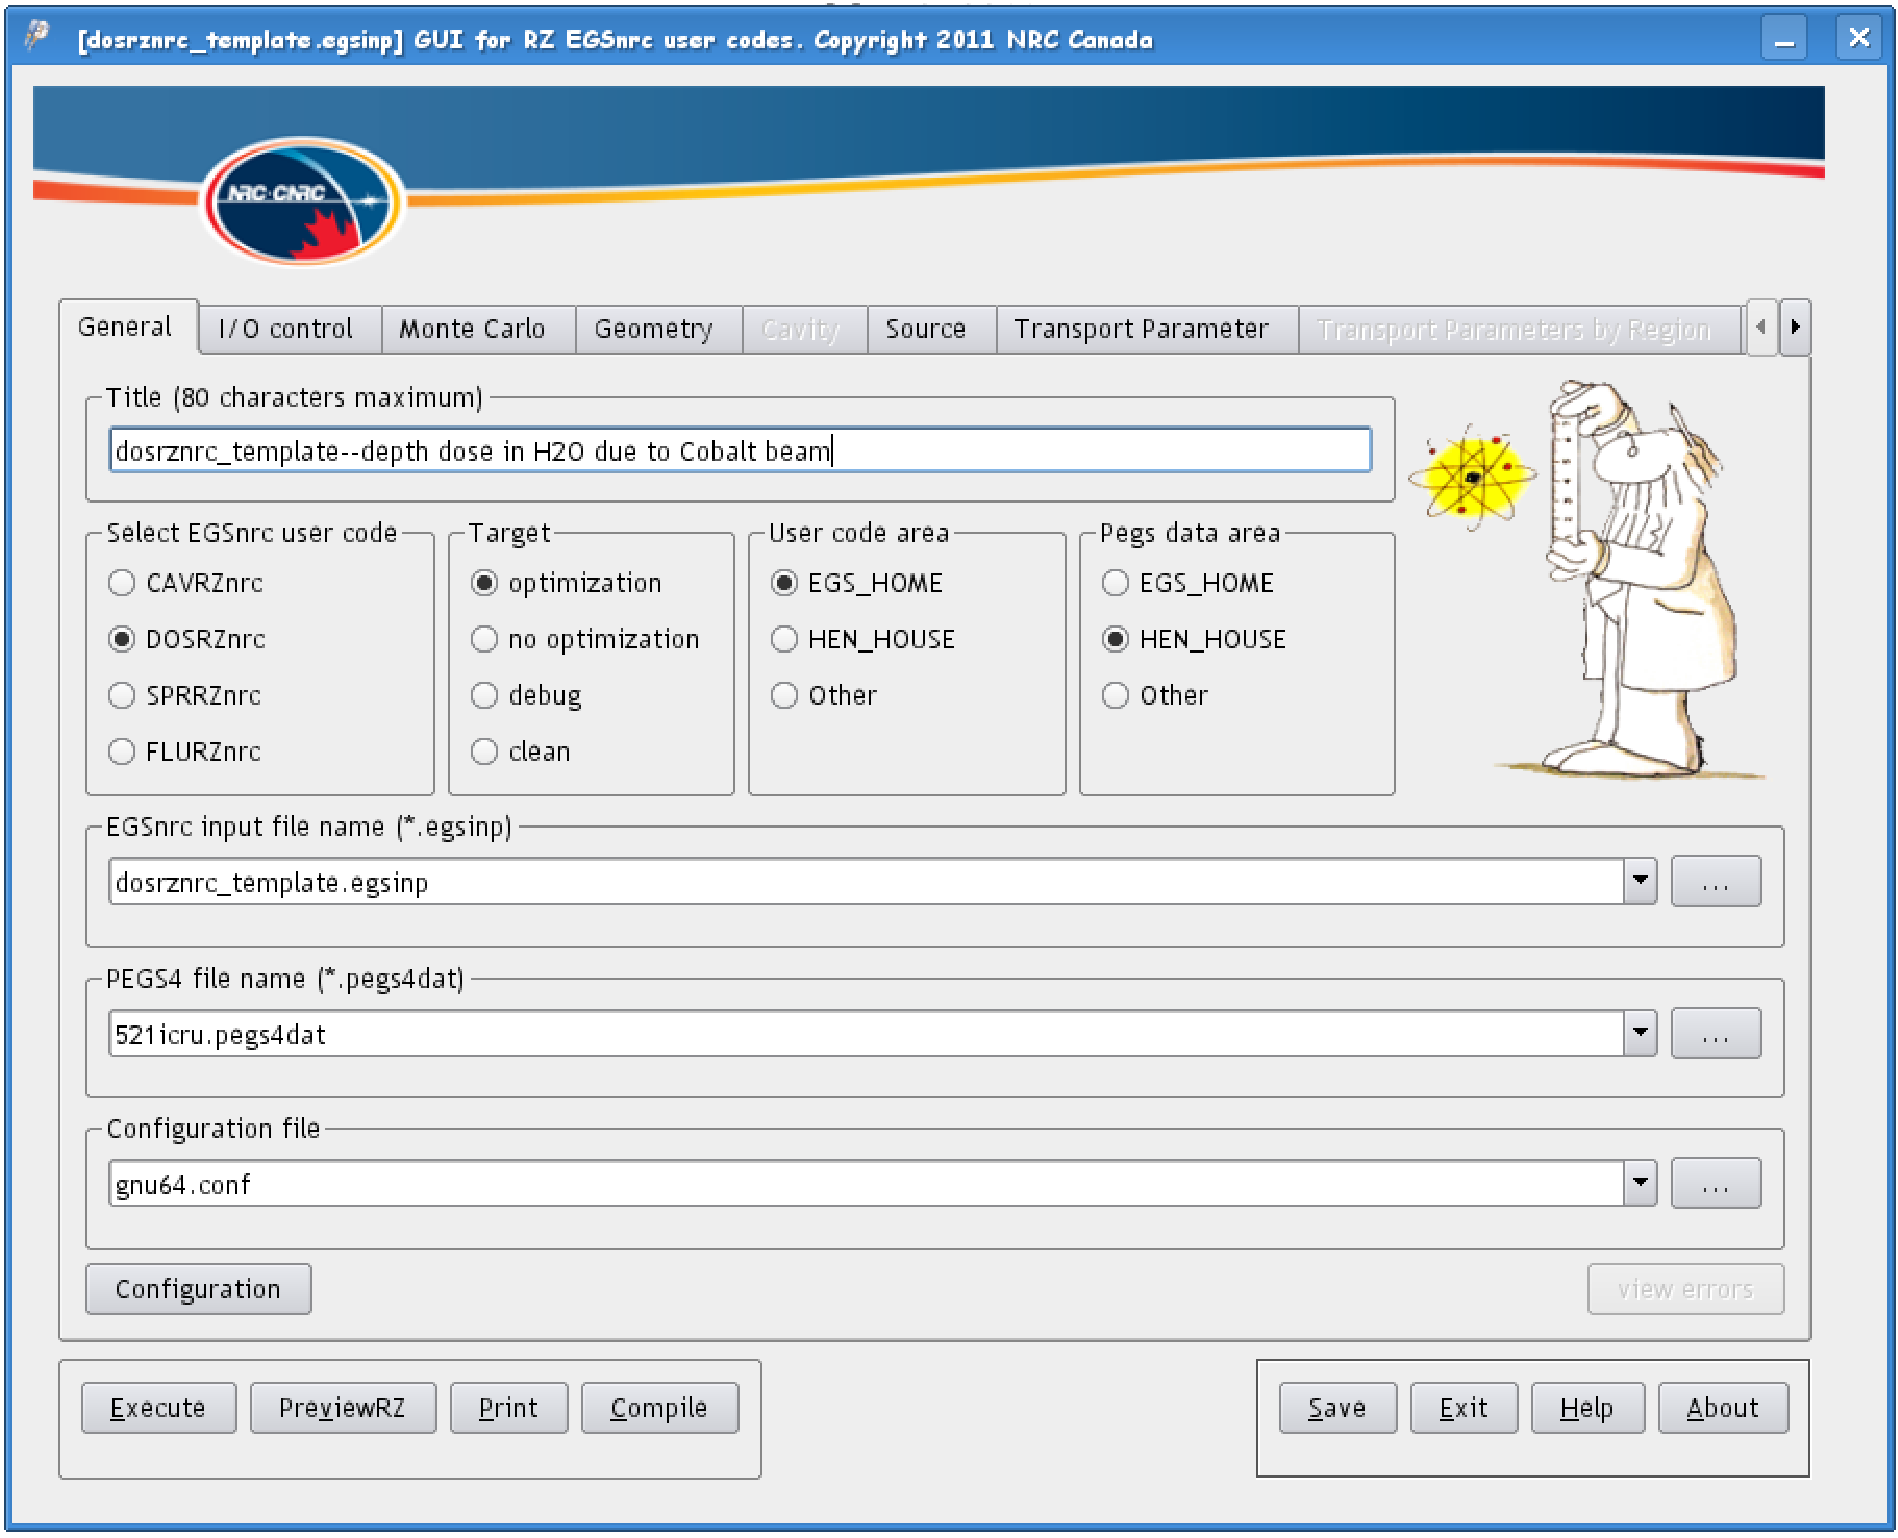
\includegraphics[height=11cm]{figures/main_page}
\vspace{5mm}
\\Front page of the egs\_inprz GUI for the RZ EGSnrc User Codes.
\vspace{10mm}\\
\end{center}
\end{latexonly}
\begin{htmlonly}
\begin{rawhtml}
<center>
<img src="figures/main_page.png">
<br><br>
Front page of the egs\_inprz GUI for the RZ EGSnrc User Codes.
<br>
</center>
\end{rawhtml}
\end{htmlonly}

\supcopyright NRC Canada, 2015

\end{center}
\newpage   %Blank page behind cover
\mbox{}

%\note{This page is intentionally blank to be the back of the front cover.
%Remove this note prior to printing!!!}


%\setcounter{page}{319}
\pagestyle{empty}

\pagestyle{fancy}



\newpage
\begin{abstract}

This is the reference user manual for {\bf \tt egs\_inprz}, a graphical user interface
for the EGSnrc RZ user-codes suite. It briefly introduces the GUI and describes how
to install it and work with it. Descriptions and snapshots of each of the input blocks
are provided.

\end{abstract}



\noindent
This code is distributed under the GNU Affero General Public License 3.0.


\tableofcontents


\newpage

\section{Introduction}

One of the major improvements in the RZ user-codes was moving from an input format
based on a long series of numbers to a text based input which is easier to use.
This text based system for input files was then used to create a single routine
({\tt get\_inputs}) to read inputs entries for all the user codes so that now
one can cut and paste entire input blocks from one user code to another.
This routine is now part of the EGSnrc system and can be used in any user-code to
parse through {\tt key=value} pairs in an input file.
As a consecuence, input files look very similar and,
more importantly, they are much easier to read and know exactly what the simulation
is about without having the description of the inputs open on the desk.
The idea behind using a GUI for working with EGSnrc input files is to further
extend the above mentioned improvements. Although the input files are currently
very readable, one must still remember what the keys used in an input file mean.
By using this GUI, a user can immediately get a description about any input parameter
by means of tool-tips.

{\tt egs\_inprz} is a Graphical User Interface (GUI), originally created for manipulating
(reading, creating, modifying, printing and visualizing)
input files for the  RZ suite of EGSnrc  user-codes:
DOSRZnrc, CAVRZnrc, SPRRZnrc and FLURZnrc (see NRCC report PIRS-702\cite{Ro10}).
Furthermore it can be also used for compiling and executing these user-codes.
% There is also an option for creating new configurations (combinations of compiler settings
% with platform specific libraries).
% \index{config files}
\index{RZ user-codes}
 {\tt egs\_inprz} is user friendly, offering more flexibility, on-line help and therefore,
increases the efficiency in getting hands-on experience with the EGSnrc user codes.

 This GUI was developed using Qt, a multi-platform, C++ Graphical User Interfaces toolkit
 that enables building efficient, portable and maintainable GUI applications
 quickly and easily. Qt is a fully object-oriented, easily extensible C++ application
 framework that enables rapid building of state-of-the-art GUI applications. For more
 information please see \htmladdnormallink{{\sf
 http://www.qt.io/.}}
{http://http://www.qt.io/}
\index{Trolltech}
\index{Qt library}


\newpage
\section{Installation}
\label{installation}

\index{installation}

\index{EGSnrcMP}
This GUI is part of the multi-platform version\cite{Ka03}
of the EGSnrc Monte Carlo simulation system\cite{Ka09a}.
For its development we used the Qt library and therefore,
users wanting to build it, will have to install this library. Most Linux distributions include the
Qt library these days, since the popular Desktop Environment KDE is based on this library. However,
if the Qt library is not available in the user's system, one needs to install it first

Only Linux/Unix users need to built this GUI since it is distributed as a binary executable on
Windows. We might start distributing binary executables for Linux/Unix as well in the near future.
The only requirement for this to happen is that most Linux distributions and Unixes are binary
compatible and the GUI is linked statically to the Qt library.

\index{KDE}
\index{Qt INSTALL file}



\subsection{Building {\tt egs\_inprz}}
\label{building}
\index{QTDIR}
\index{building egs\_inprz}

\index{compiling {\tt egs\_inprz}}
The user can have this and the other GUI's built during installation of the EGSnrc system,
provided {\tt QTDIR} is properly set. At any time the user can go to
{\tt \$HEN\_HOUSE/gui/egs\_inprz} and type

      {\tt ./make [EGS\_CONFIG=desired\_config]}

\noindent A C++ compiler will have to be installed on
your computer in order to build the GUIs.
On Windows one {\bf must} have installed either MS C++ 6.0 or Borland C++.

\noindent {\bf Note:} You only need to pass {\tt EGS\_CONFIG} to {\tt make} if it is not set
or you want/need to build the GUI for a different configuration as the current one.
In principle, all Makefiles provided in the new EGSnrcMP environment are for {\tt GNU make}.
Although they might also work with other Unix {\tt make} versions.

It is important that the environment variable {\tt QTDIR} points to the location where
Qt was installed. This can be checked by issuing the command:

      {\tt echo \$QTDIR} on Unix/Linux or

      {\tt echo \%QTDIR\%} on a Windows console.

One can change this environment variable by issuing the command

      {\tt setenv QTDIR Qt\_location} for the C shell, or

      {\tt export QTDIR = Qt\_location} for Bash, or

      {\tt set QTDIR=Qt\_location} on a Windows console.

{\bf On Unix/Linux} this variable can be set on a system wide basis by including the
corresponding statement above in the {\tt .cshrc} resource file for the C-shell or
the {\tt .basrc} resource file for Bash.

{\bf On Windows} the user can also set the QTDIR environment variable system wide by
right clicking on the {\tt My Computer} icon, selecting {\tt Properties} and clicking on the
{\tt Environment Variables} button in the {\tt Advanced} tab.

\newpage
\section{Using {\tt egs\_inprz}}
\subsection{Running {\tt egs\_inprz}}
\index{executing}
\index{HEN\_HOUSE}

After installing EGSnrc, {\tt egs\_inprz} is located on {\tt HEN\_HOUSE/bin/my\_machine/}.
{\tt my\_machine} stands for the name of the configuration used to build the GUI. For more
information about configurations the user is referred to the PIRS-877 report on the new
multi-platform environment\cite{Ka03}.

{\bf On Windows} the user can invoke directly the binary executable from a DOS console, since its
location will be on the user's PATH environment variable. If requested by the user, there will
be also shortcuts to the GUI's distributed with the EGSnrc system on the Desktop and
Start Menu.
\index{executing!Windows}

{\bf On Unix/Linux} the user can also invoke directly the binary executable from a shell console,
since its location is added to the user's PATH environment variable when the corresponding
{\tt egsnrc\_[cshrc|bashrc]\_additions} is sourced, which {\bf must} have been done after
installing the EGSnrc system.
The alias {\tt egsinprz} is
also available, which points to {\tt HEN\_HOUSE/bin/my\_machine/egs\_inprz} and starts the GUI
in the background.
If requested by the user, shortcuts for the KDE desktop environment are also created by the
installation GUI.
\index{executing!Unix/Linux}

Once all the necessary information is entered, the user can perform different operations
from within the GUI provided the input file has been saved to the disk since all other
operations use the disk version of the input file.


\subsection{Reading EGSnrc RZ input files}
\label{reading}
\index{input files!reading}

Existing input files can be read directly from the command line by passing the file name as
argument, i.e., by invoking

        {\tt egs\_inprz} {\em filename[.egsinp]}

\noindent
where the file name can be with or without extension. If the file does not exist, a warning
message is shown and the file name {\tt new\_file.egsinp} is used instead. Note, that in this
case no input file will exist. To have an actual input file and be able to run a calculation,
the user {\bf must} have saved it. Saving {\tt new\_file.egsinp} without modifying any entry
will leave a default input file for use with the RZ user code {\tt dosrznrc.mortran}.

Once an existing input file is loaded, it is
searched to identify the user-code it belongs to. If no user-code is identified,
DOSRZnrc is used by default. Once the user-code to be used is known, its location
becomes the place where the GUI will look for input files.

Regarding location, the EGSnrc system relies on having the input file on the EGSnrc
user area, \ie, {\tt EGS\_HOME/user-code}. This is so because for execution,
temporary directories and output files are created, moved and deleted and all these
operations are relative to the {\tt EGS\_HOME/user-code} location.

For this reason, this GUI will only store input files in the user's EGSnrc
area, i.e., {\tt EGS\_HOME/user-code}. If the EGSnrc user area does not exist,
the GUI creates it and issues a warning.
\index{input files!location}
\index{EGS\_HOME}

Input files can be also read in from the GUI's General tab. Once the GUI is loaded,
a list of available {\em *.egsinp} input files in the current directory is offered
to the user through the EGSnrc input file name combo box. By default the input file
template {\em dosrznrc\_template.egsinp}, distributed with the EGSnrc system, is loaded.
Alternatively, the user can click on the button to the right of the combo box to
invoke an open file dialog to open any {\em *.egsinp} file located anywhere.
\index{.egsinp}

The GUI verifies that all media used in the input file are available in the selected
PEGS4 data set. By default this file is set to be {\tt 521icru.pegs4dat}, a standard data
file, that comes with the EGSnrc distribution. If any medium is not found in the
current PEGS4 data file, an error message pops up recommending that the user corrects the
media names and/or find the appropriate data file.
\index{PEGS4}
\index{pegs4 media}

\index{user-code area}
The user-code area is the location where {\tt egs\_inprz} will look for input files. Initially,
{\tt egs\_inprz} assumes that the user-code area is {\tt EGS\_HOME/user-code}, where {\tt user-code}
is by default {\em dosrznrc}. If the GUI is started from any user-code location, {\tt user-code}
is changed to the corresponding user-code. If a valid input file name is passed as argument to
{\tt egs\_inprz}, then after identifying the user-code, {\tt user-code} is updated properly.
The user-code area can
be later changed by the user in the general input tab (see figure \ref{generalfig} in section
\ref{general}).

\index{PEGS4-data area}
Similarly, the PEGS4 data area is the location where {\tt egs\_inprz} will look for PEGS4 data sets.
Since
there are some data sets in the EGSnrc distribution, we chose to set this area to be in
{\tt HEN\_HOUSE/pegs4/data} by default. Later on, when users have created their own data sets, they
can switch to {\tt EGS\_HOME/pegs4/data} or any other location of their preference.


\subsection{Creating EGSnrc RZ input files}
\label{creating }
\index{input files!creating}

As mentioned above, when starting the RZ GUI, the template {\tt dosrznrc\_template.egsinp} is
read in, which contains defaults for all possible entries. Saving this template under any other
name is a possible way for getting started. In similar fashion, one can switch to another RZ
user-code (see section \ref{general}) and select the corresponding input template file.
\index{default input file}

\subsection{Porting input files between NRC RZ user-codes}
\label{modifying}
\index{input files!porting}

 Sometimes different user-codes share common input blocks like transport parameters,
 geometry, variance reduction parameters, and so on. For instance,
 the user might want to run a CAVRZnrc calculation to obtain the dose inside the air
 cavity of an ion chamber and also run a FLURZnrc calculation to obtain the spectrum
 inside the cavity for the same chamber. This is easily acomplished with {\tt egs\_inprz}
 by loading the input file for the CAVRZnrc calculation, switching to the other user
 code input by  clicking on the corresponding radio button in
 the user-code group box (see figure \ref{generalfig} in section \ref{general}).
One will have to modify the default entries for the selected user-code to suit the user's
problem if needed. Once the proper entries are made, the input file can be saved by
clicking on the {\em Save} or {\em Save\&Exit} button
in the user's EGSnrc user-code area (if it doesn't exist, it is created automatically,
 and a warning is issued to the user).\\

\subsection{Viewing the geometry with previewRZ}
\index{previewRZ}
\index{geometry!visualizing}
\index{input files!previewRZ}

Once an existing input file has been loaded or created from scratch and saved on
the hard drive,
the user can invoke
{\tt previewRZ}, a tool supplied with the EGSnrc distribution, which allows one
to visualize the geometry and material data (see figure \ref{view}).
The {\tt PreviewRZ} button, placed in the left bottom corner of the GUI
(see any GUI snapshot in section \ref{screenshots}),
becomes enabled if Tcl/Tk is installed on your computer, the input file exists
and there were no errors reading the geometry. Pressing this button is equivalent
to typing on the command line of a console (Windows or Unix/Linux)

 {\tt HEN\_HOUSE/previewRZ/previewRZ name[.egsinp]}

\noindent where the input filename can be entered with or without extension. \\

\begin{figure}[h]
\begin{htmlonly}
\begin{rawhtml}
<p><center>
<img width=486 height=629 src="figures/previewrz.png"><br><br>
</center>
\end{rawhtml}
\end{htmlonly}
\begin{latexonly}
\begin{center}
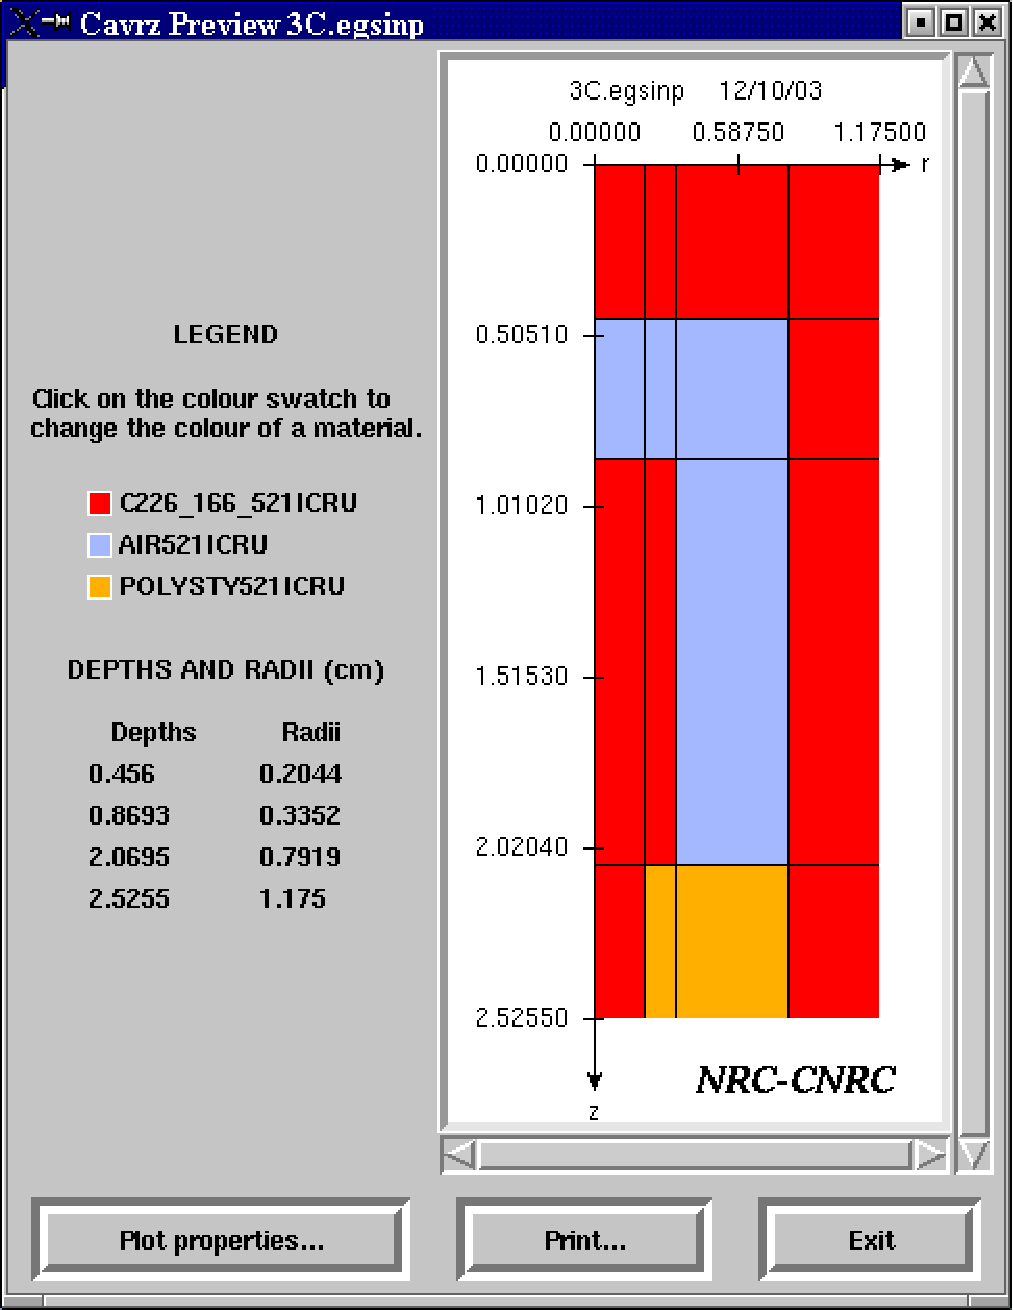
\includegraphics[height=9cm]{figures/previewrz}
\end{center}
\end{latexonly}
\begin{center}

\includegraphics[height=1mm]{figures/fake2}
\end{center}
\caption{View of a 3C cylindrical ionization chamber using {\tt previewRZ}.}
\label{view}
\end{figure}

{\tt previewRZ} is a Tcl/Tk script
which had been previously used at NRC only on Unix/Linux. We have now successfully used
{\tt previewRZ} on Windows 2000/XP after downloading and installing a Tcl/Tk
self-extracting distribution.
To find out whether
Tcl/Tk is available on the user's system, {\tt egs\_inprz} tries to find the binary
executable {\tt wish.exe} on Windows or {\tt wish} on Unix/Linux in any of the locations
defined on the user's PATH environment
variable.
The Tcl/Tk package is {\bf FREELY} distributed for HP-UX, Linux,
Solaris, and Windows by ActiveState Corp.
To obtain  Tcl/Tk go to
\htmladdnormallink{{\sf
 http://www.activestate.com/Products/ActiveTcl/}}
{http://www.activestate.com/Products/ActiveTcl/}
and click on the {\tt Download} link of the page. For more information and useful links
on Tcl/Tk please visit
\htmladdnormallink{{\sf
http://www.tcl.tk/software/tcltk/}}
{http://www.tcl.tk/software/tcltk/}
\index{Tcl/Tk}
\index{Active State Corp.}
\index{wish}

Future versions of the {\tt egs\_inprz} GUI will use its own
previewing tool, but for now, users wishing to have the feature of looking
at the geometry they are defining, will have to install the Tcl/Tk package.

\subsection{Printing *.egsinp input files}
\index{input files!printing}

 To produce a hard copy of the input file, users have the option to print the file
 by pressing the {\tt Print} button located in the button group on the lower left
 corner of the GUI (see any GUI snapshot in section \ref{screenshots}). A Print
 Dialog pops up with a list of available printers and a printer and  paper format
 setup among other options (see figure \ref{print}).\\

\begin{figure}[htb]
\begin{htmlonly}
\begin{rawhtml}
<p><center>
<img width=517 height=606 src="figures/printer_dialog.png" name=print><br><br>
</center>
\end{rawhtml}
\end{htmlonly}
\begin{latexonly}
\begin{center}
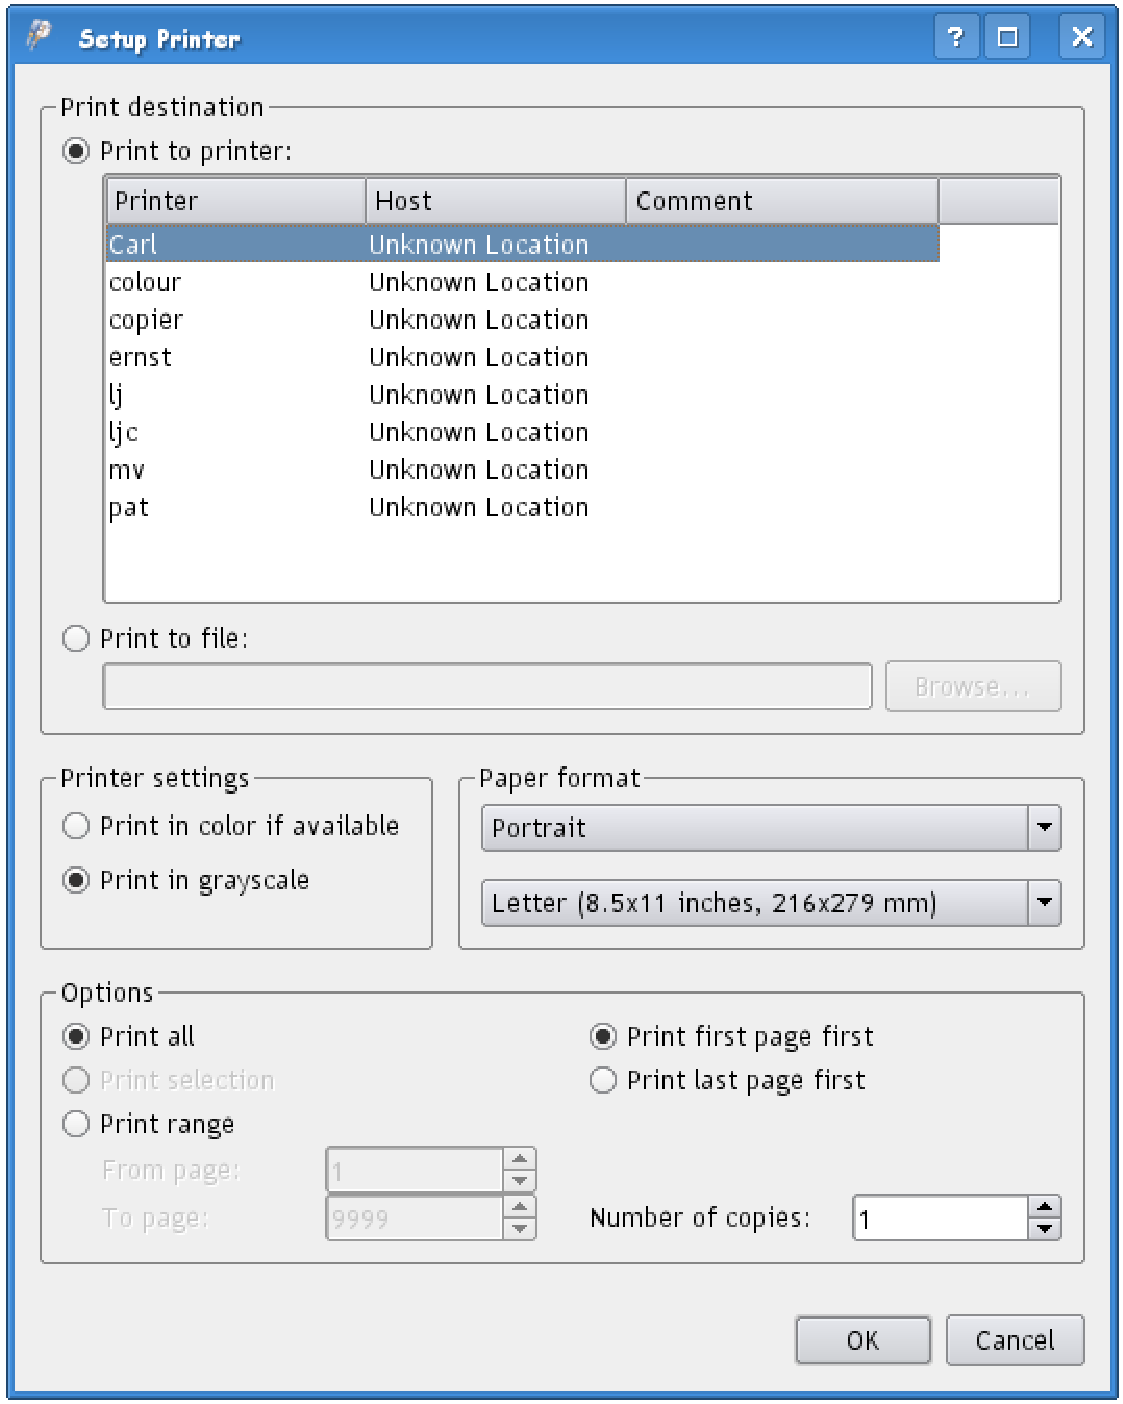
\includegraphics[height=9cm]{figures/printer_dialog}
\end{center}
\end{latexonly}
\begin{center}

\includegraphics[height=1mm]{figures/fake2}
\end{center}
\caption{\label{print}Printer Setup Dialog on SuSE Linux 10.3 KDE 3.5.9}
\end{figure}

\subsection{Compiling the RZ user codes}

When one modifies the user-codes, these need to be re-compiled.
The user can perform
this operation from within the GUI by pressing the {\em Compile} button on the  lower left
corner of the GUI (see for instance figure \ref{generalfig} in section \ref{general}).
On the {\tt General Information} tab there is a {\tt Target} radio button group box where
one can choose the type of compilation desired. By default it is set to {\tt optimization}
which uses the optimization option defined in the active config file generated during the
EGSnrc installation process or the configuration utility available in all the EGSnrcMP GUI's.
The other available options are {\tt no optimization, debug and clean}.
Optimization is recommended for production runs after the user-code
and the input file have been thoroughly tested.

\subsection{Executing the RZ user codes}

After all necessary information has been entered and stored, one can execute the EGSnrc
RZ user-code from within the GUI by pressing the {\em Execute} button on the  lower left
corner of the GUI (see figure \ref{generalfig} in section \ref{general}). A dialog appears
where one can define the different execution parameters (see figure \ref{execution}).
There are two modes for running an EGSnrc RZ user-code, {\it interactive} or {\it batch}, \ie,
using a batch queuing system. The execution mode defaults to {\it interactive}.
The {\it batch} execution mode is only available on Unix/Linux since it has not
been implemented on Windows yet.
At NRC the {\em PBS batch system} is currently used to send jobs to a queue where
they are remotely executed, returning the results after completion to the
user EGSnrc area.

% \begin{figure}[tbp]
\begin{figure}[h]
\begin{htmlonly}
\begin{rawhtml}
<p><center>
<img src="figures/execution.png" name=execution><br><br>
</center>
\end{rawhtml}
\end{htmlonly}
\begin{latexonly}
\begin{center}
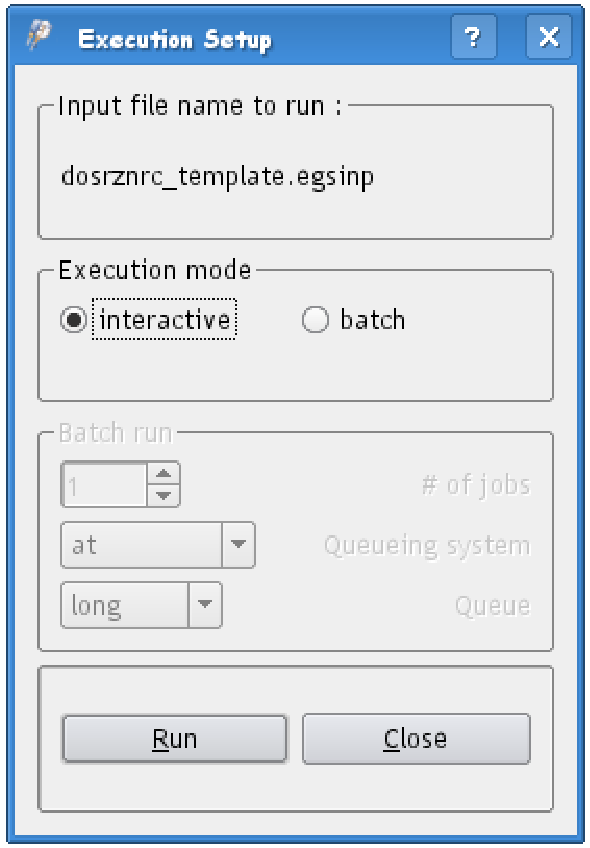
\includegraphics[height=11cm]{figures/execution}
\end{center}
\end{latexonly}
\begin{center}

\includegraphics[height=1mm]{figures/fake2}
\end{center}
\caption{Execution Setup Dialog.}
\label{execution}
\end{figure}

{\bf On Unix/Linux} if the batch execution mode is selected, a pane becomes enabled where
queue input parameters can be entered such as the queueing system, type of queue
and number of jobs to submit (see figure \ref{batchexecution}).
The GUI recognizes which queueing systems are available
by looking up on {\tt \$HEN\_HOUSE/scripts} for batch definition files in the form
{\tt batch\_options.queueing\_system},
where {\tt queueing\_system} stands for either {\tt at}, {\tt nqs} or {\tt pbs}. The user
can add any other batch submission system by creating a batch definition file in a similar
fashion to the ones in the EGSnrcMP distribution.

The default batch submission system assumed in the GUI is the standard Unix
job submission tool {\tt at}. The batch definition files provided in the directory
{\tt \$HEN\_HOUSE/scripts} contain specific definitions for the {\tt at},
{\tt NQS} and {\tt PBS} batch submission systems. If the user wants to make NQS, PBS or
any other system the default job submission system,
he/she can define the environment variable {\tt EGS\_BATCH\_SYSTEM} to be nqs, pbs or
the name of the other queueing system.
\index{EGS\_BATCH\_SYSTEM}
\index{queueing system}
\index{batch runs}
\index{batch\_options}

These are the batch definition files distributed with the EGSnrc system:
\begin{description}
\item {\tt batch\_options.at}
\item {\tt batch\_options.nqs}
\item {\tt batch\_options.pbs}
\end{description}
\index{batch\_options}
\index{queueing system}

Queue names are installation especific and at NRC the
names {\em short}, {\em medium} and {\em long} have been adopted for {\tt PBS} and {\tt NQS}.
To change these, edit the names
in the proper batch definition file.

For more information on the implementation of parallel runs in the new EGSnrc system, the reader
is refered to the NRCC report PIRS-877.

\begin{figure}[h]
\begin{htmlonly}
\begin{rawhtml}
<p><center>
<img src="figures/execution_batch.png" name=batchexecution><br><br>
</center>
\end{rawhtml}
\end{htmlonly}
\begin{latexonly}
\begin{center}
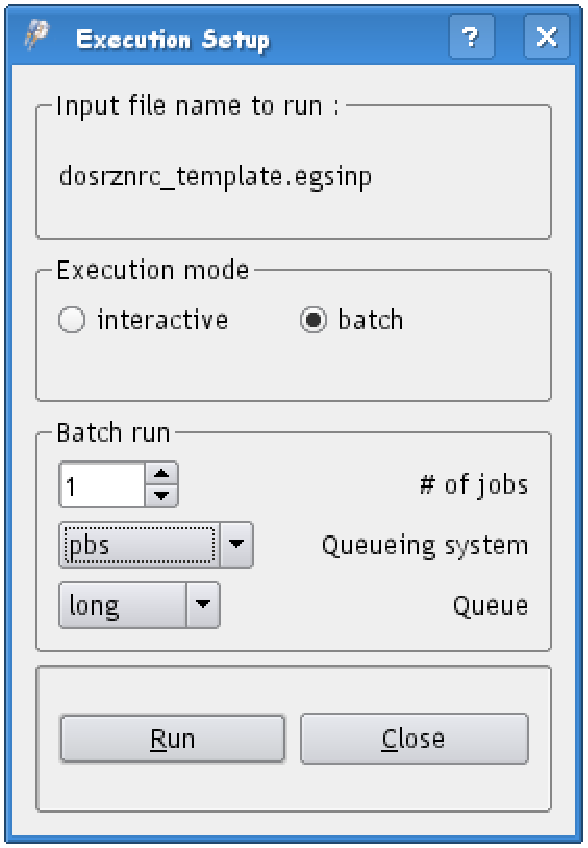
\includegraphics[height=11cm]{figures/execution_batch}
\end{center}
\end{latexonly}
\begin{center}

\includegraphics[height=1mm]{figures/fake2}
\end{center}
\caption{Execution Setup Dialog in batch mode.}
\label{batchexecution}
\end{figure}

\clearpage

%
% \section{Creating and modifying config files}
%
% A key element in the new EGSnrcMP multi-platform environment is the config file,
% which contains important system definitions allowing the use of EGSnrc on different
% Operating Systems and with different compilers. A detailed description of config
% files and definition of what constitutes a configuration can be found in the technical
% report PIRS-877\cite{Ka03}.
%
% \begin{figure}[htb]
% \begin{htmlonly}
% \begin{rawhtml}
% <p><center>
% <img src="figures/configure.png" name=config><br><br>
% </center>
% \end{rawhtml}
% \end{htmlonly}
% \begin{latexonly}
% \begin{center}
% 
\includegraphics[height=10cm]{figures/configure.png}
% \end{center}
% \end{latexonly}
% \begin{center}
% 
\includegraphics[height=1mm]{figures/fake2}
% \end{center}
% \caption{Configuration Wizard.}
% \label{config}
% \end{figure}
%
% From within {\tt egs\_inprz}, users can modify existing config files and
% create new ones by clicking on the {\tt Configuration} button found on the General
% Information tab. A reduced version of the {\tt egs\_install} Wizard appears where
% one can define the Fortran and C compilers and set the names for the config file and
% the configuration (figure \ref{config}). Once all the required information has been
% entered, the Wizard
% runs a series of tests for the selected Fortran and C compilers on the running
% operating system. The
% results of these tests are used to create the system/compiler dependent
% files {\tt machine.mortran} and {\tt machine.macros}.  The configuration
% utility then starts the actual building of the EGSnrc system, by
% creating the Mortran3 string processor {\tt mortran3.exe} and the PEGS4
% data pre-processing tool {\tt pegs4.exe}.

\section{Getting help}
\label{help}

One of the advantages of a graphical user interface is the possibility of providing
information in an interactive way. {\tt egs\_inprz} uses this feature extensively by
activating so called {\em tool tips} when the user positions the mouse over a given area
in the GUI. A dialog pops up {\em temporarily} with information, if available, about the
corresponding input quantity.

There is also the possibility of activating these {\em tool tips} {\em permanently} (until
another action is performed: mouse click or key press). For this, the user must set the focus
on the relevant location and press {\tt Shift+F1}. The help text appears immediately; it goes
away as soon as the user does something else.

More general information is provided in html format through the {\em Help} button located
in the lower right corner of the GUI ({\em html} version of this document).
{\tt egs\_inprz} attemps to run {\em Internet Explorer} on Windows and
{\em Konqueror} or {\em Netscape} on Unix/Linux to show the document. If none of these
are available an error message is displayed. In that case the user can go to {\tt \$HEN\_HOUSE/gui/egs\_inprz/html} and load the index page {\em index.html} with an html
browser of his/her choice.

\section{Input blocks description and screenshots}
\label{screenshots}

In this section we describe briefly the different input blocks that are used in the NRC
RZ user codes.
We have also included screenshots of the different input tabs of the GUI. In each
of these tabs, there are input options, common to all the RZ user codes. But some of them are
specific to one user code and remain disabled when one selects a different user code.
The active file name is always displayed on the GUI's caption. This can be useful to recognize
whether the current file name in the input box is the same as the active one.

{\bf Note} that the bottom row of buttons are available with all tabs.


\newpage
\subsection{The General Information Tab}
\label{general}

As its name suggests, this section of the tabbed dialog is intended to collect general
information not contemplated inside the input file itself like the input and pegs4 data
file names, the areas to search for those files, compilation mode, execution mode and
its parameters,
the user code name, etc. The title constitutes an exception, since it is part of the input
file, but does not fit in any of the different input blocks.

A very useful feature in this GUI is the ability to set the location of the input and
pegs4 files automatically to be in the {\tt HEN\_HOUSE} or {\tt EGS\_HOME} area. This saves
time by not having to browse all the way to the location of different files, acting like
a shortcut. If the files are loaded from a location different than the above
mentioned, the {\tt Other} radio button is checked. Note that upon loading an input file
from a location other than the {\tt HEN\_HOUSE} or {\tt EGS\_HOME} user code area, it will
be only saved on the {\tt EGS\_HOME} user code area. \\ \\
\begin{figure}[htb]
\begin{htmlonly}
\begin{rawhtml}
<p><center>
<img src="figures/general.png" name=generalfig><br><br>
</center>
\end{rawhtml}
\end{htmlonly}
\begin{latexonly}
\begin{center}
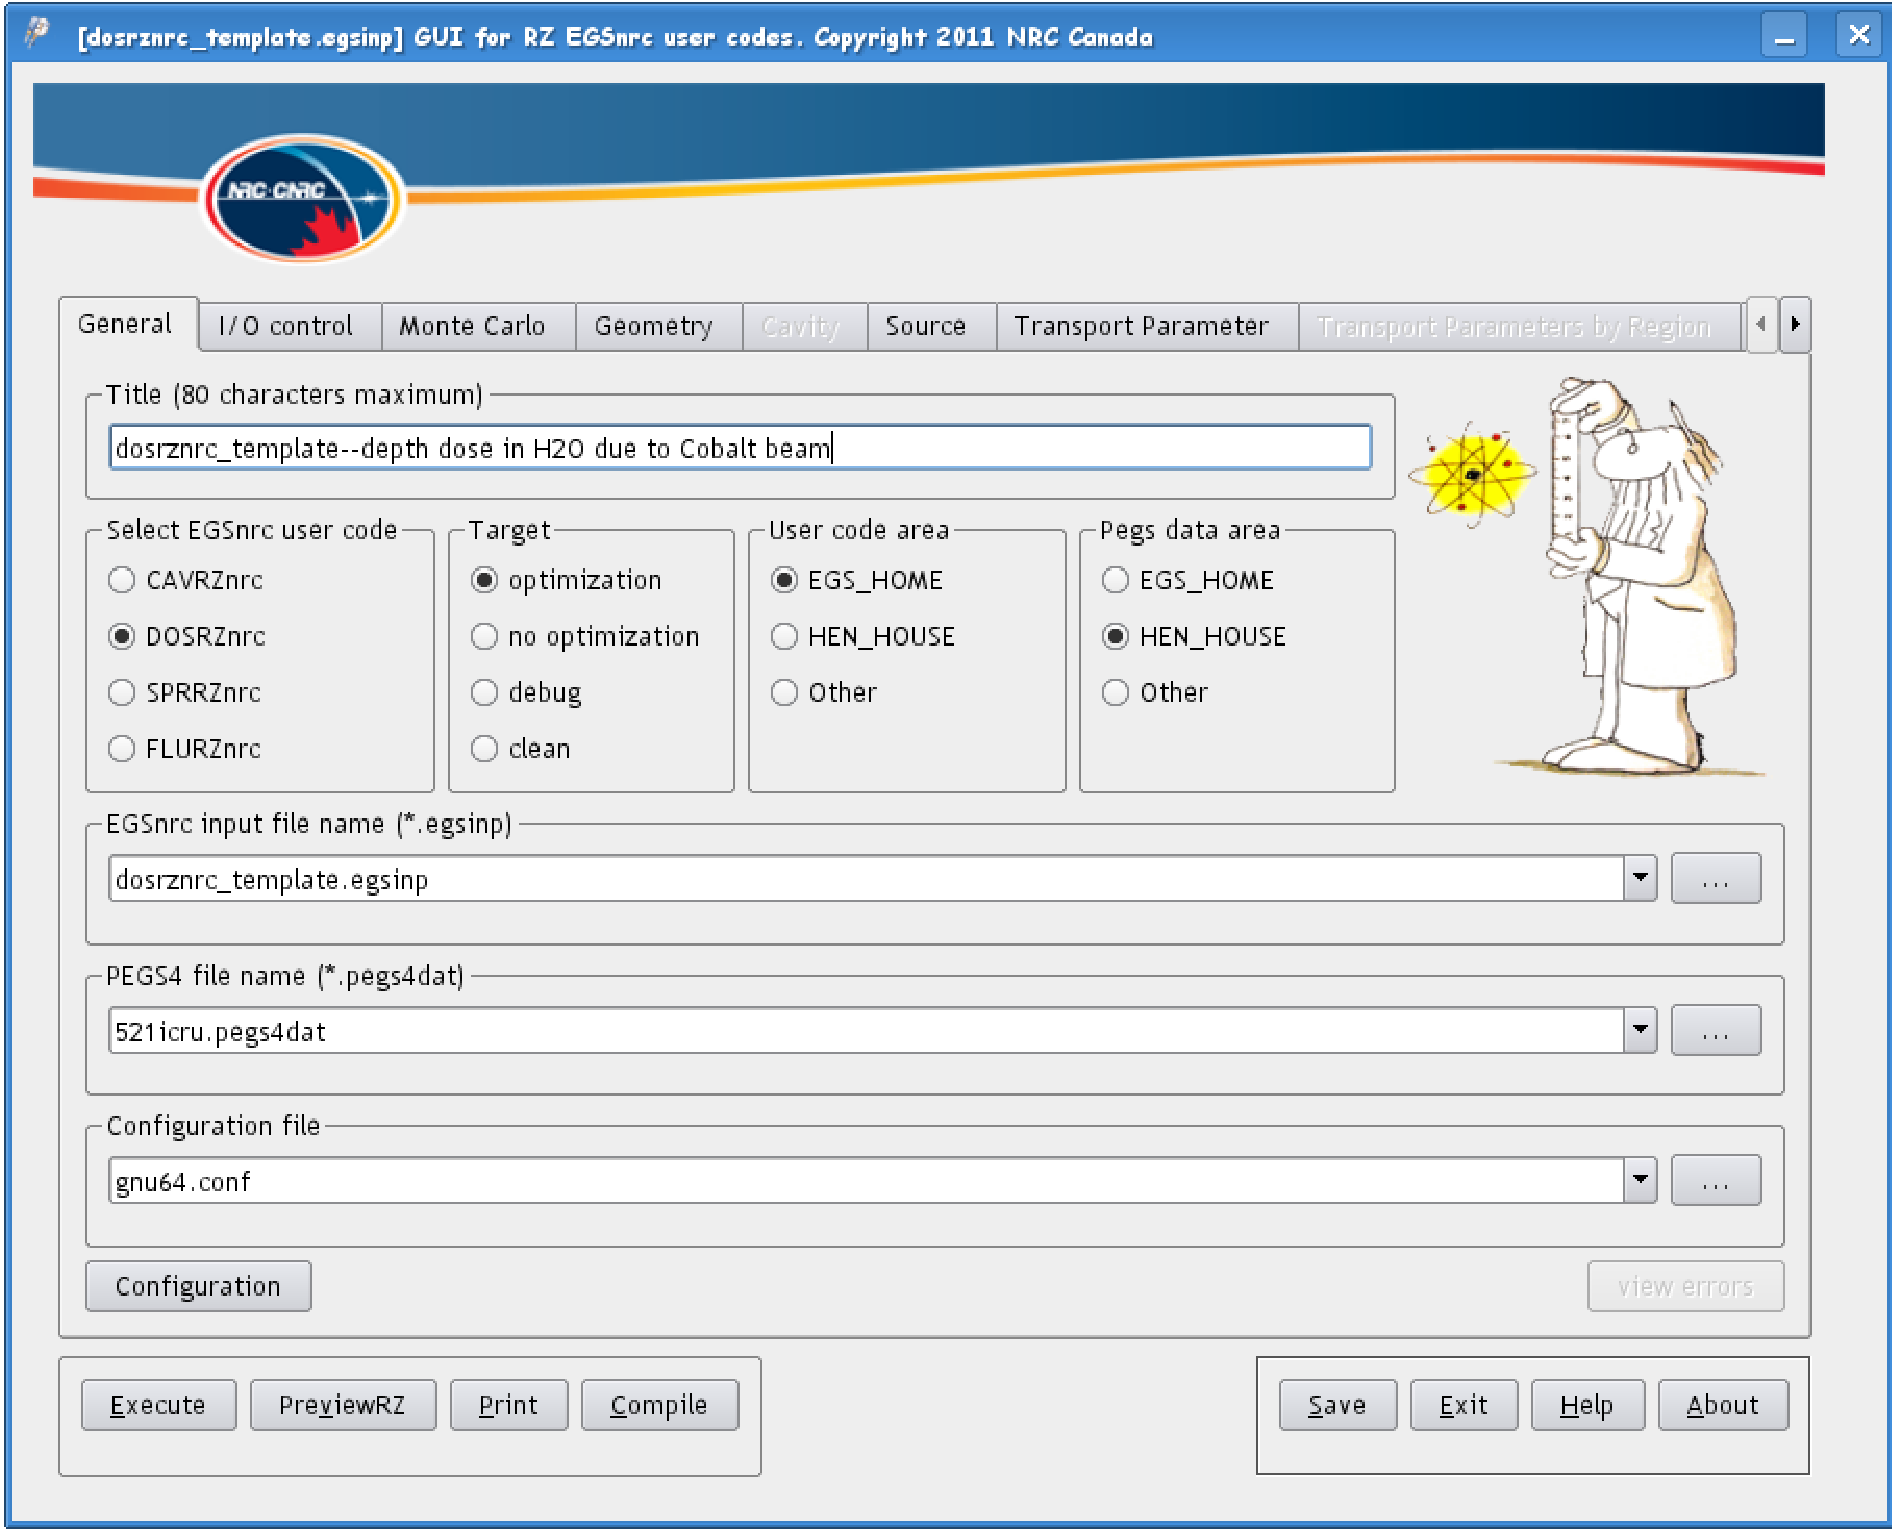
\includegraphics[height=10.78cm]{figures/general}
\end{center}
\end{latexonly}
\begin{center}

\includegraphics[height=1mm]{figures/fake2}
\end{center}
\caption{General Input for the RZ EGSnrc User Codes.}
\label{generalfig}
\end{figure}

\newpage
\subsection{The I/O Control Tab}
\label{io}

This block contains information relevant to the I/O controls of the NRC user codes.
Many of the inputs are common to all codes, but there are some which are specific to
only some of them. \\ \\
\begin{figure}[htb]
\begin{htmlonly}
\begin{rawhtml}
<p><center>
<img src="figures/io.png" name=io_control><br><br>
</center>
\end{rawhtml}
\end{htmlonly}
\begin{latexonly}
\begin{center}
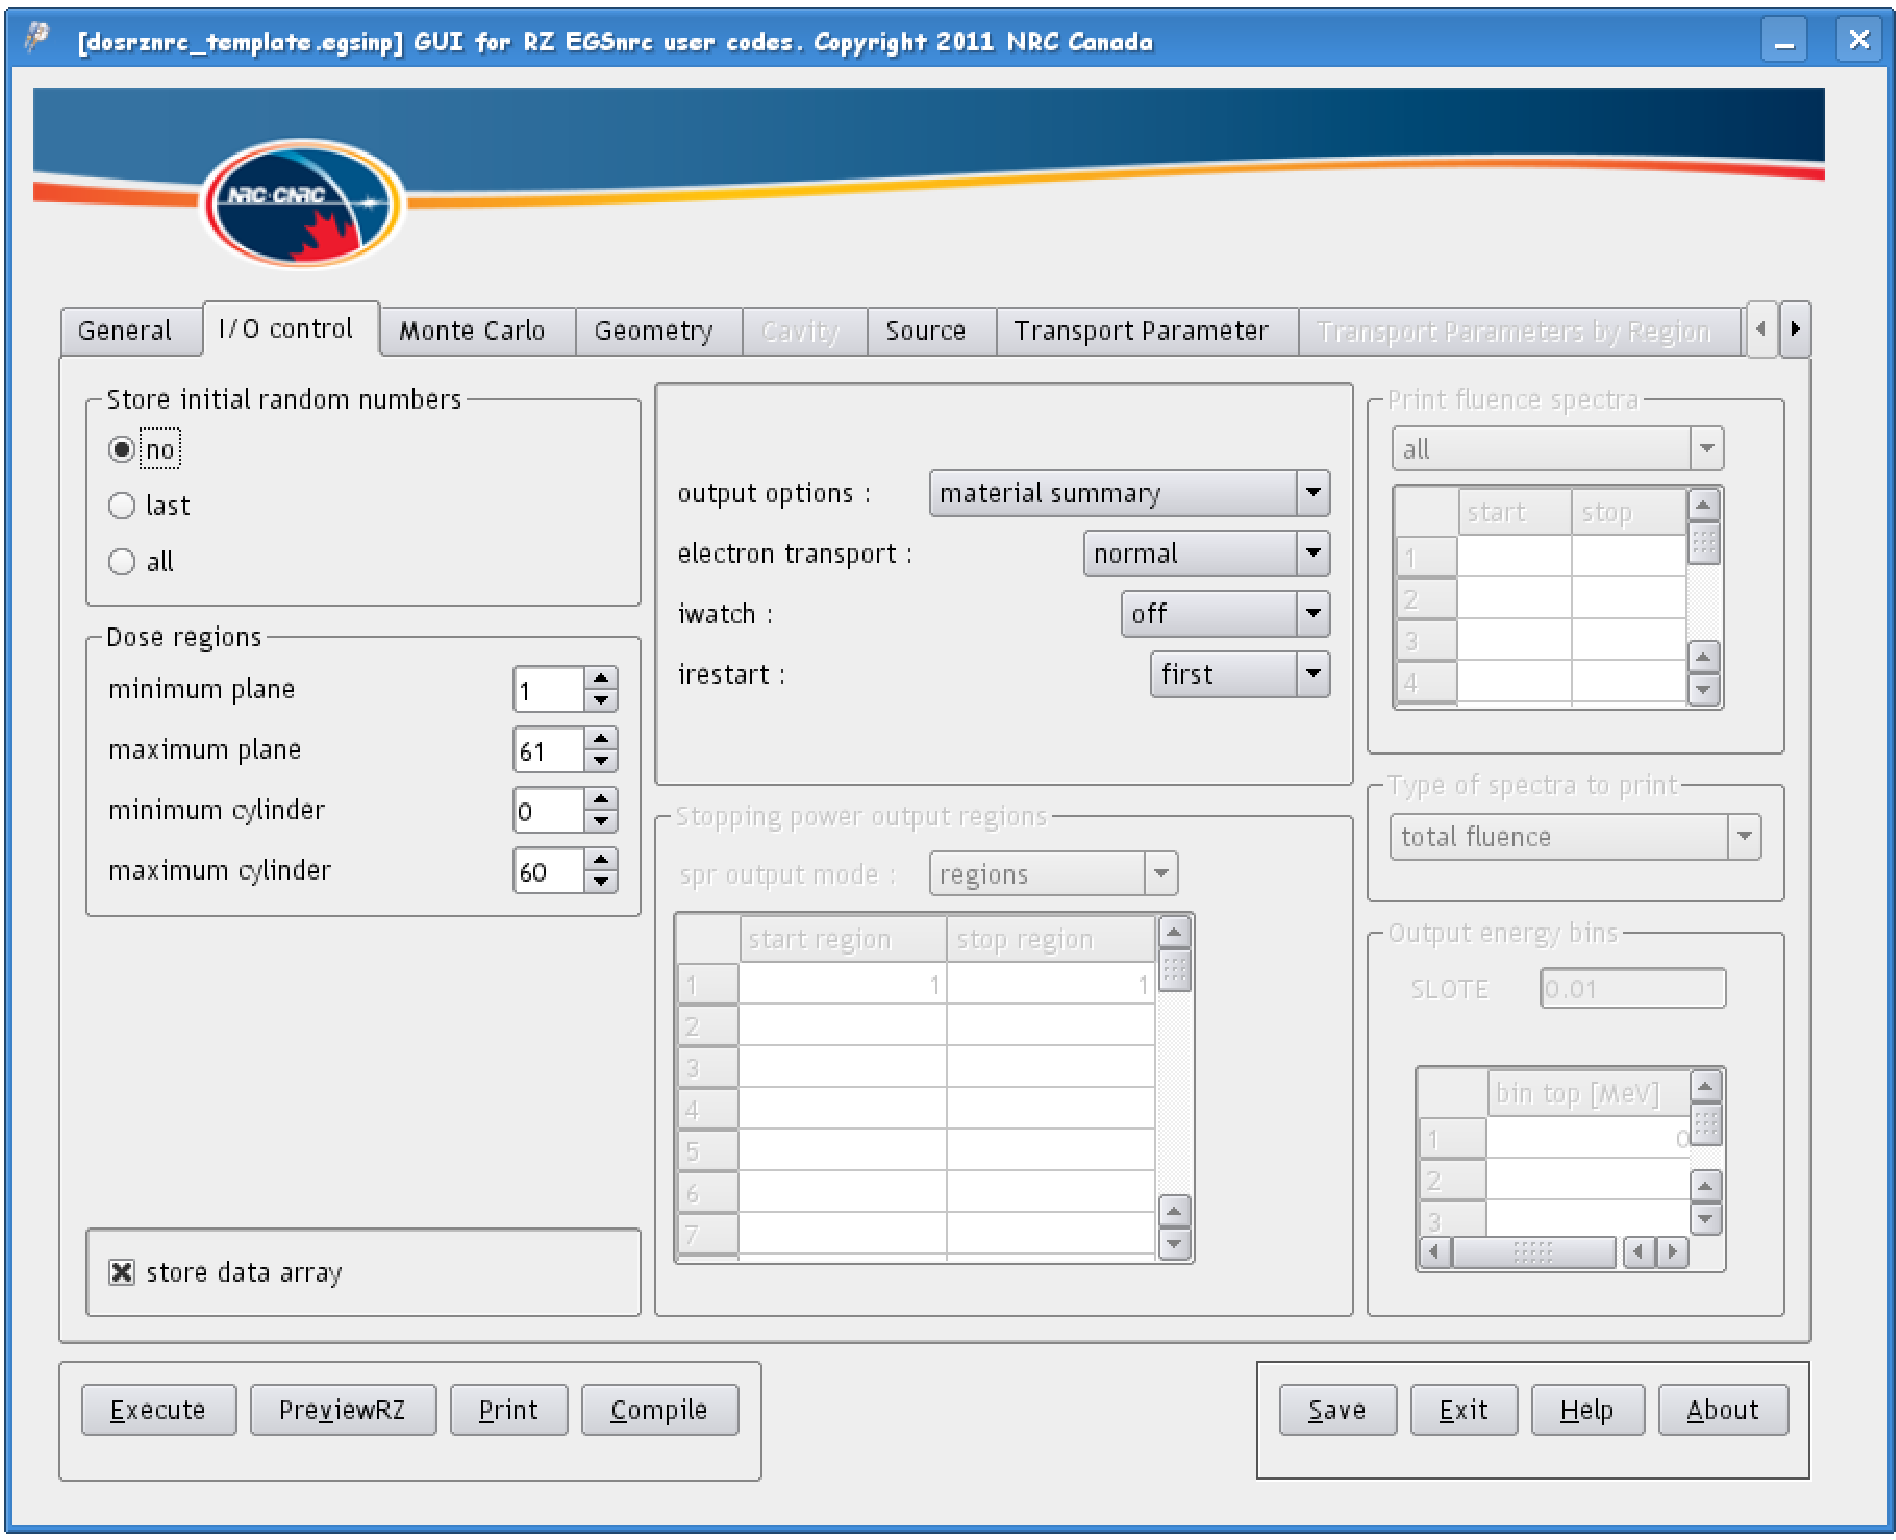
\includegraphics[height=10.78cm]{figures/io}
\end{center}
\end{latexonly}
\begin{center}

\includegraphics[height=1mm]{figures/fake2}
\end{center}
\caption{I/O control for the RZ EGSnrc User Codes.}
\label{io_control}
\end{figure}


\newpage
\subsection{The Monte Carlo Parameter Tab}
\label{mc}


This input tab collects the typical information required in a Monte Carlo simulation like
the number of histories to run, the initial random number seeds, desired statistical accuracy,
and the maximum CPU time for the calculation. There are also more user code specific entries
that are enabled or disabled depending on the user code selected.

An input block required only by the user code DOSRZnrc when the calculation type is
{\em pulse height distribution} is also included in this tab. For other calculation types and user codes,
this box remains disabled. \\ \\

% The command below does not work !!!
%\DeclareGraphicsRule{.tiff}{eps}{.tiff.bb}{'convert #1 'eps:-'}

\begin{figure}[htb]
\begin{htmlonly}
\begin{rawhtml}
<p><center>
<img src="figures/mc.png" name=mc_control><br><br>
</center>
\end{rawhtml}
\end{htmlonly}
\begin{latexonly}
\begin{center}
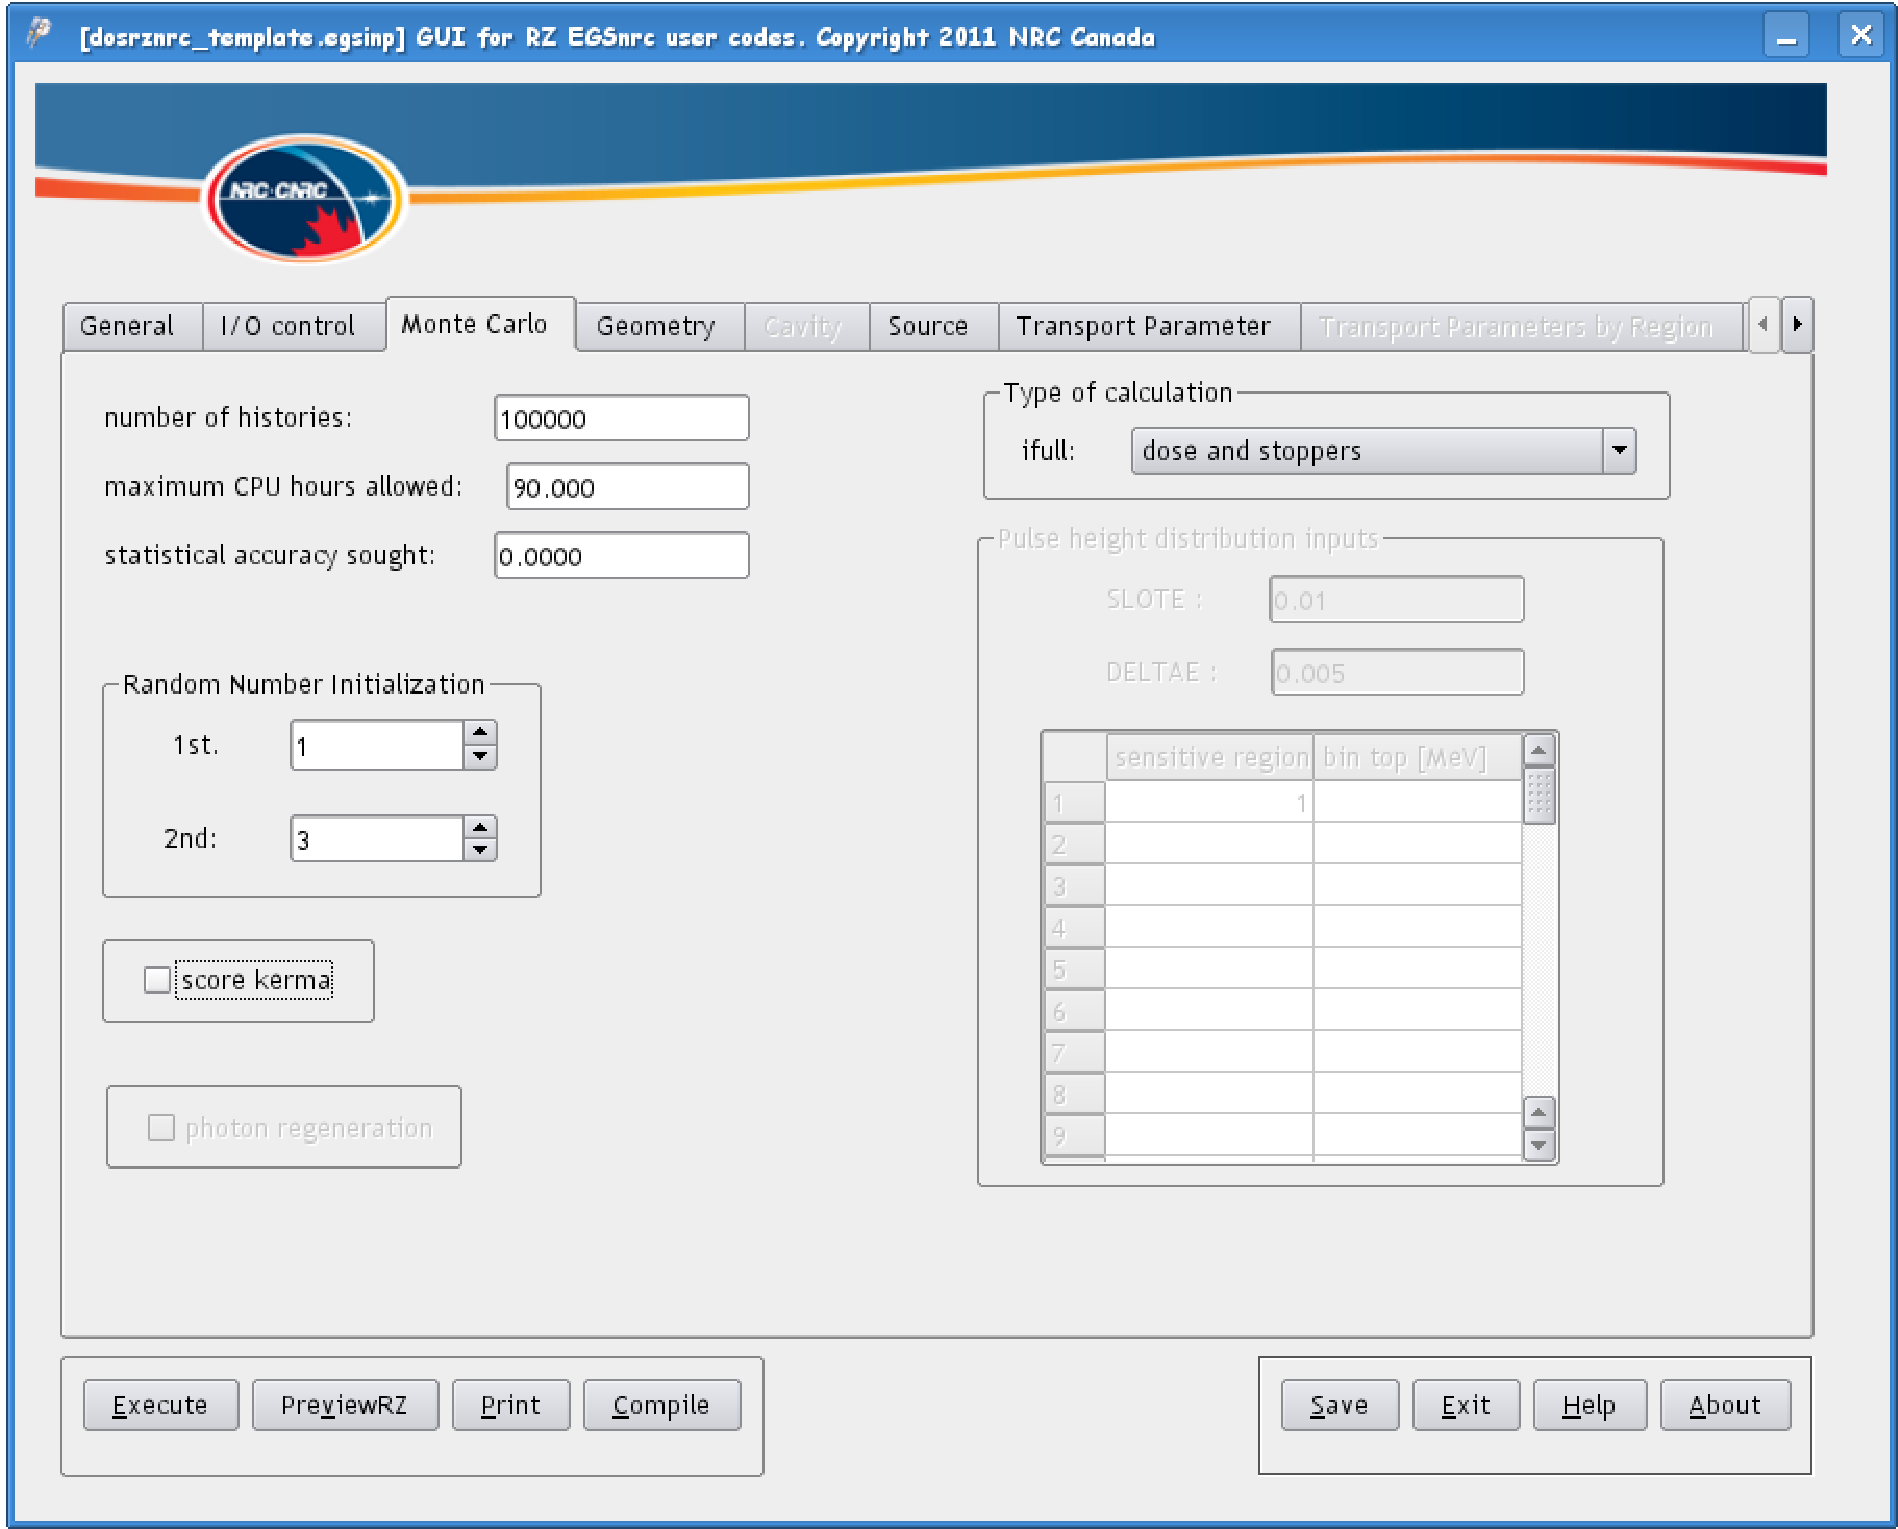
\includegraphics[height=11.56cm]{figures/mc}
\end{center}
\end{latexonly}
\begin{center}

\includegraphics[height=1mm]{figures/fake2}
\end{center}
\caption{Monte Carlo parameters for the RZ EGSnrc User Codes.}
\label{mc_control}
\end{figure}


\newpage
\subsection{The Geometry Tab}

This input block contains all the necessary inputs for defining a RZ geometry (cylindrical symmetry)
and the media present in the different regions. It is important to notice that for the user code
CAVRZnrc an option is available to define the geometry in a simpler way. If the input method selected
(upper left corner of the tab) is {\em cavity description}, then the rest of the input fields in this
tab are disabled and the whole geometry input occurs through the next tab, {\tt the cavity tab}.

Only media present in the current PEGS4 data set can be set in the media table. This is assured by
activating a combo box in the first column of the media table as soon as the user tries to type
or double click on it. \\ \\

\begin{figure}[htb]
\begin{htmlonly}
\begin{rawhtml}
<p><center>
<img src="figures/geometry.png" name=geometry_control><br><br>
</center>
\end{rawhtml}
\end{htmlonly}
\begin{latexonly}
\begin{center}
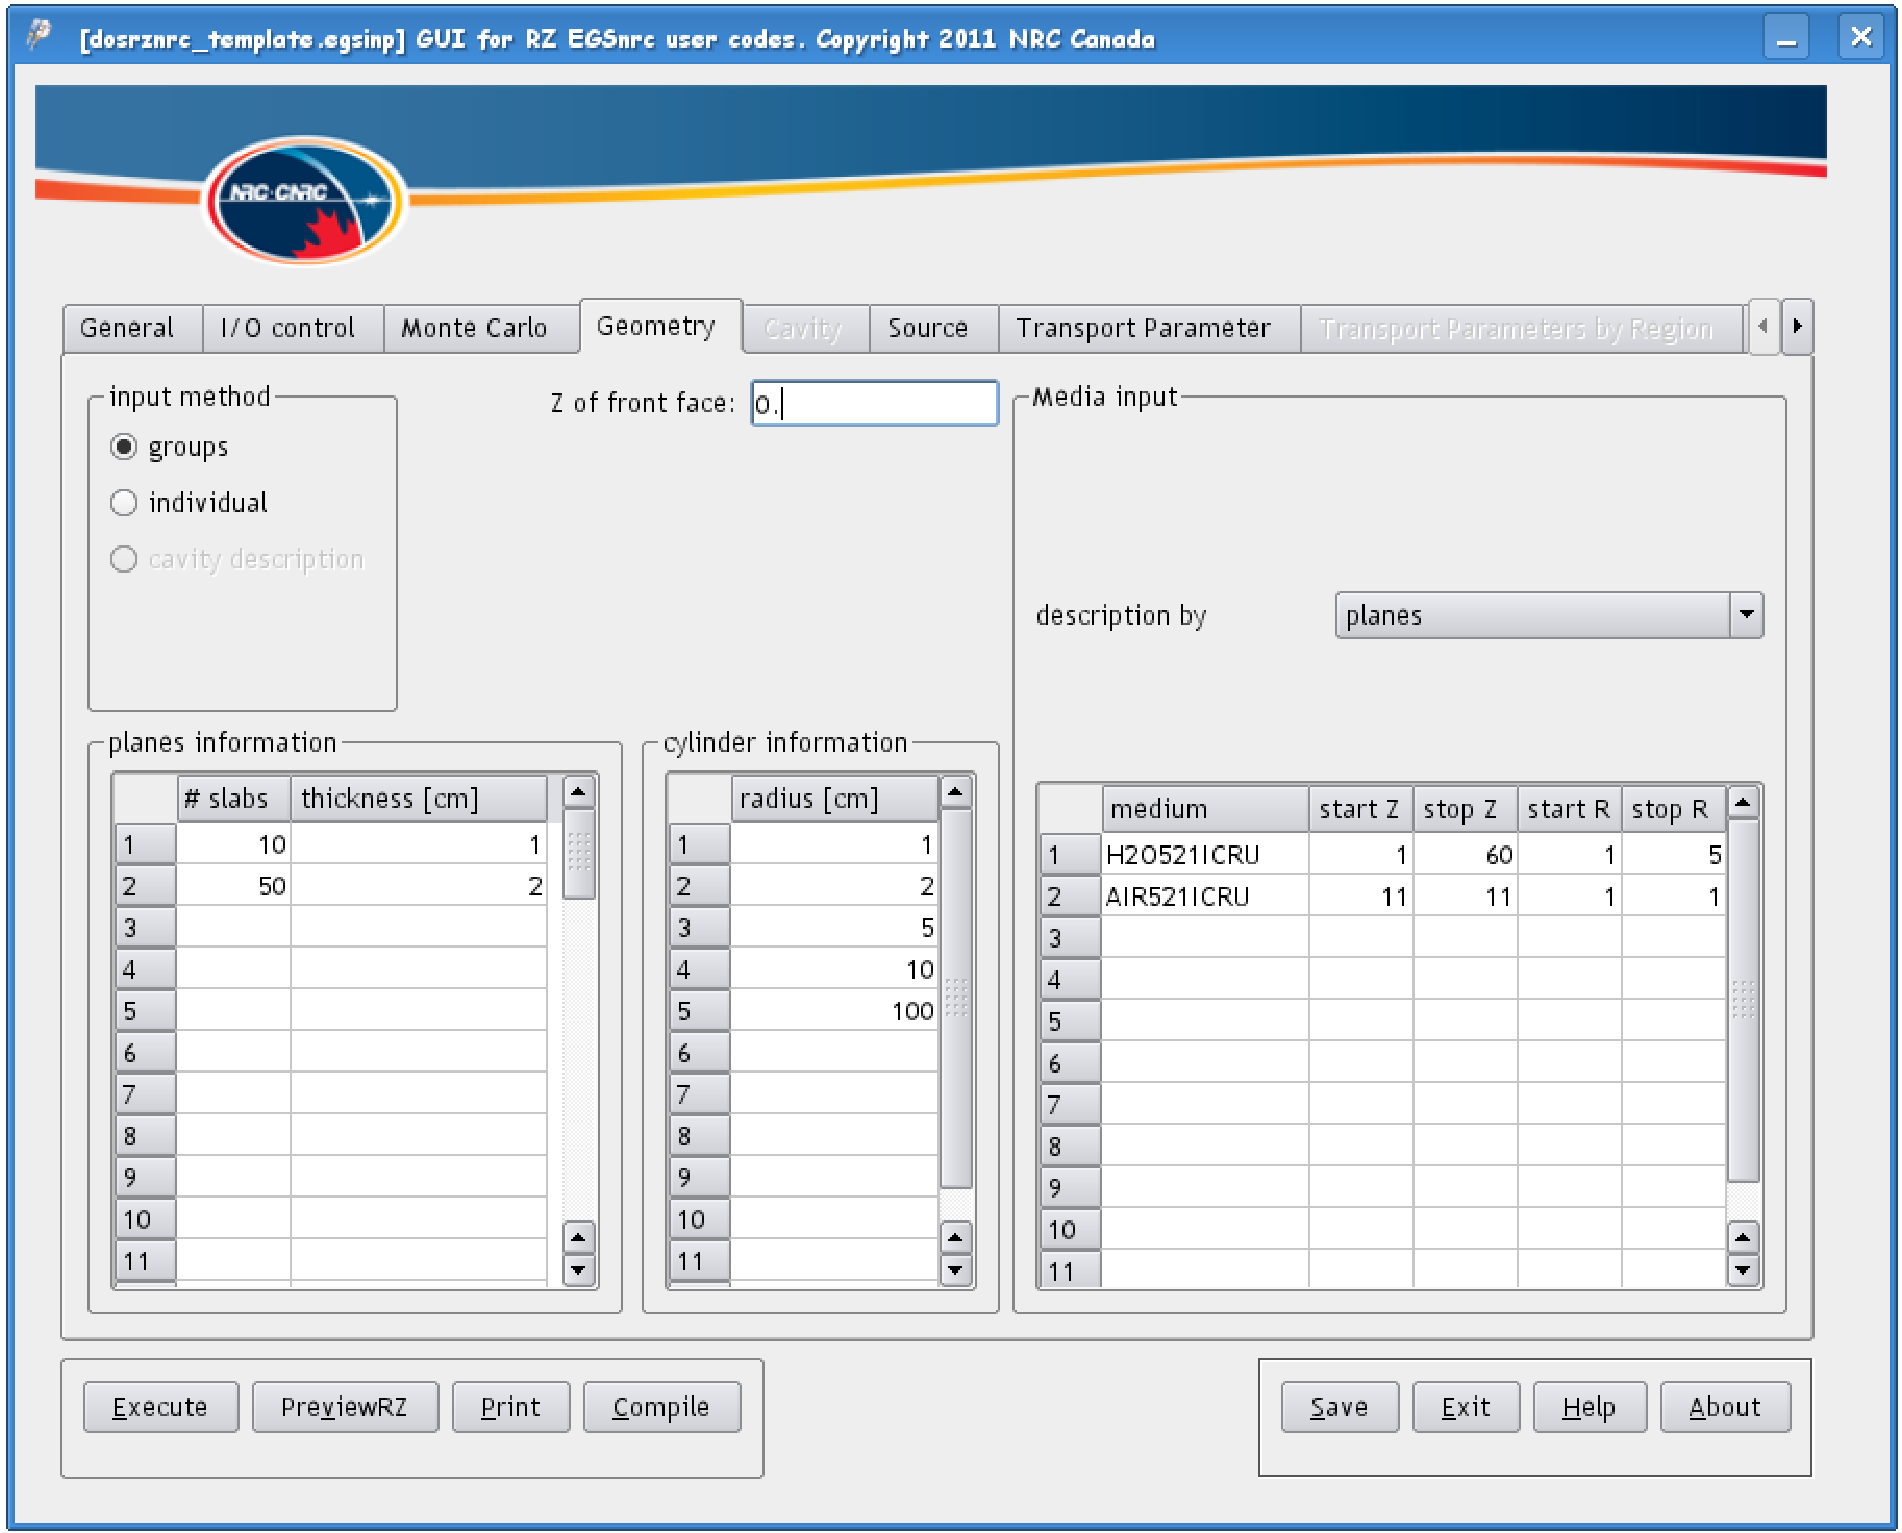
\includegraphics[height=11.56cm]{figures/geometry}
\end{center}
\end{latexonly}
\begin{center}

\includegraphics[height=1mm]{figures/fake2}
\end{center}
\caption{Geometry Input for the RZ EGSnrc User Codes.}
\label{geometry_control}
\end{figure}

\newpage
\subsection{The Cavity Tab}

This tab is only enabled for the user code CAVRZnrc. If the input method selected in the
{\tt geometry tab} (upper left corner) is {\em groups} or {\em individual}, the user can
define the regions comprising the cavity there. If on the other hand, the input method selected
is {\em cavity description}, then the rest of the input fields in the {\tt the geometry tab}
are disabled and the whole geometry input occurs here. The materials for the chamber wall
and the electrode can be selected from available media in the current PEGS4 data file.
This option was useful for early calculations but is not adequate for chambers in which one
wants to include much detail.

{\bf Beware:} If the input method is cavity description, the material name inside the cavity is
assumed to be {\bf AIR} by the user-code CAVRZnrc, \ie, CAVRZnrc will search for this medium in
the pegs4 data file. \\ \\


\begin{figure}[htb]
\begin{htmlonly}
\begin{rawhtml}
<p><center>
<img src="figures/cavity.png" name=cavity_control><br><br>
</center>
\end{rawhtml}
\end{htmlonly}
\begin{latexonly}
\begin{center}
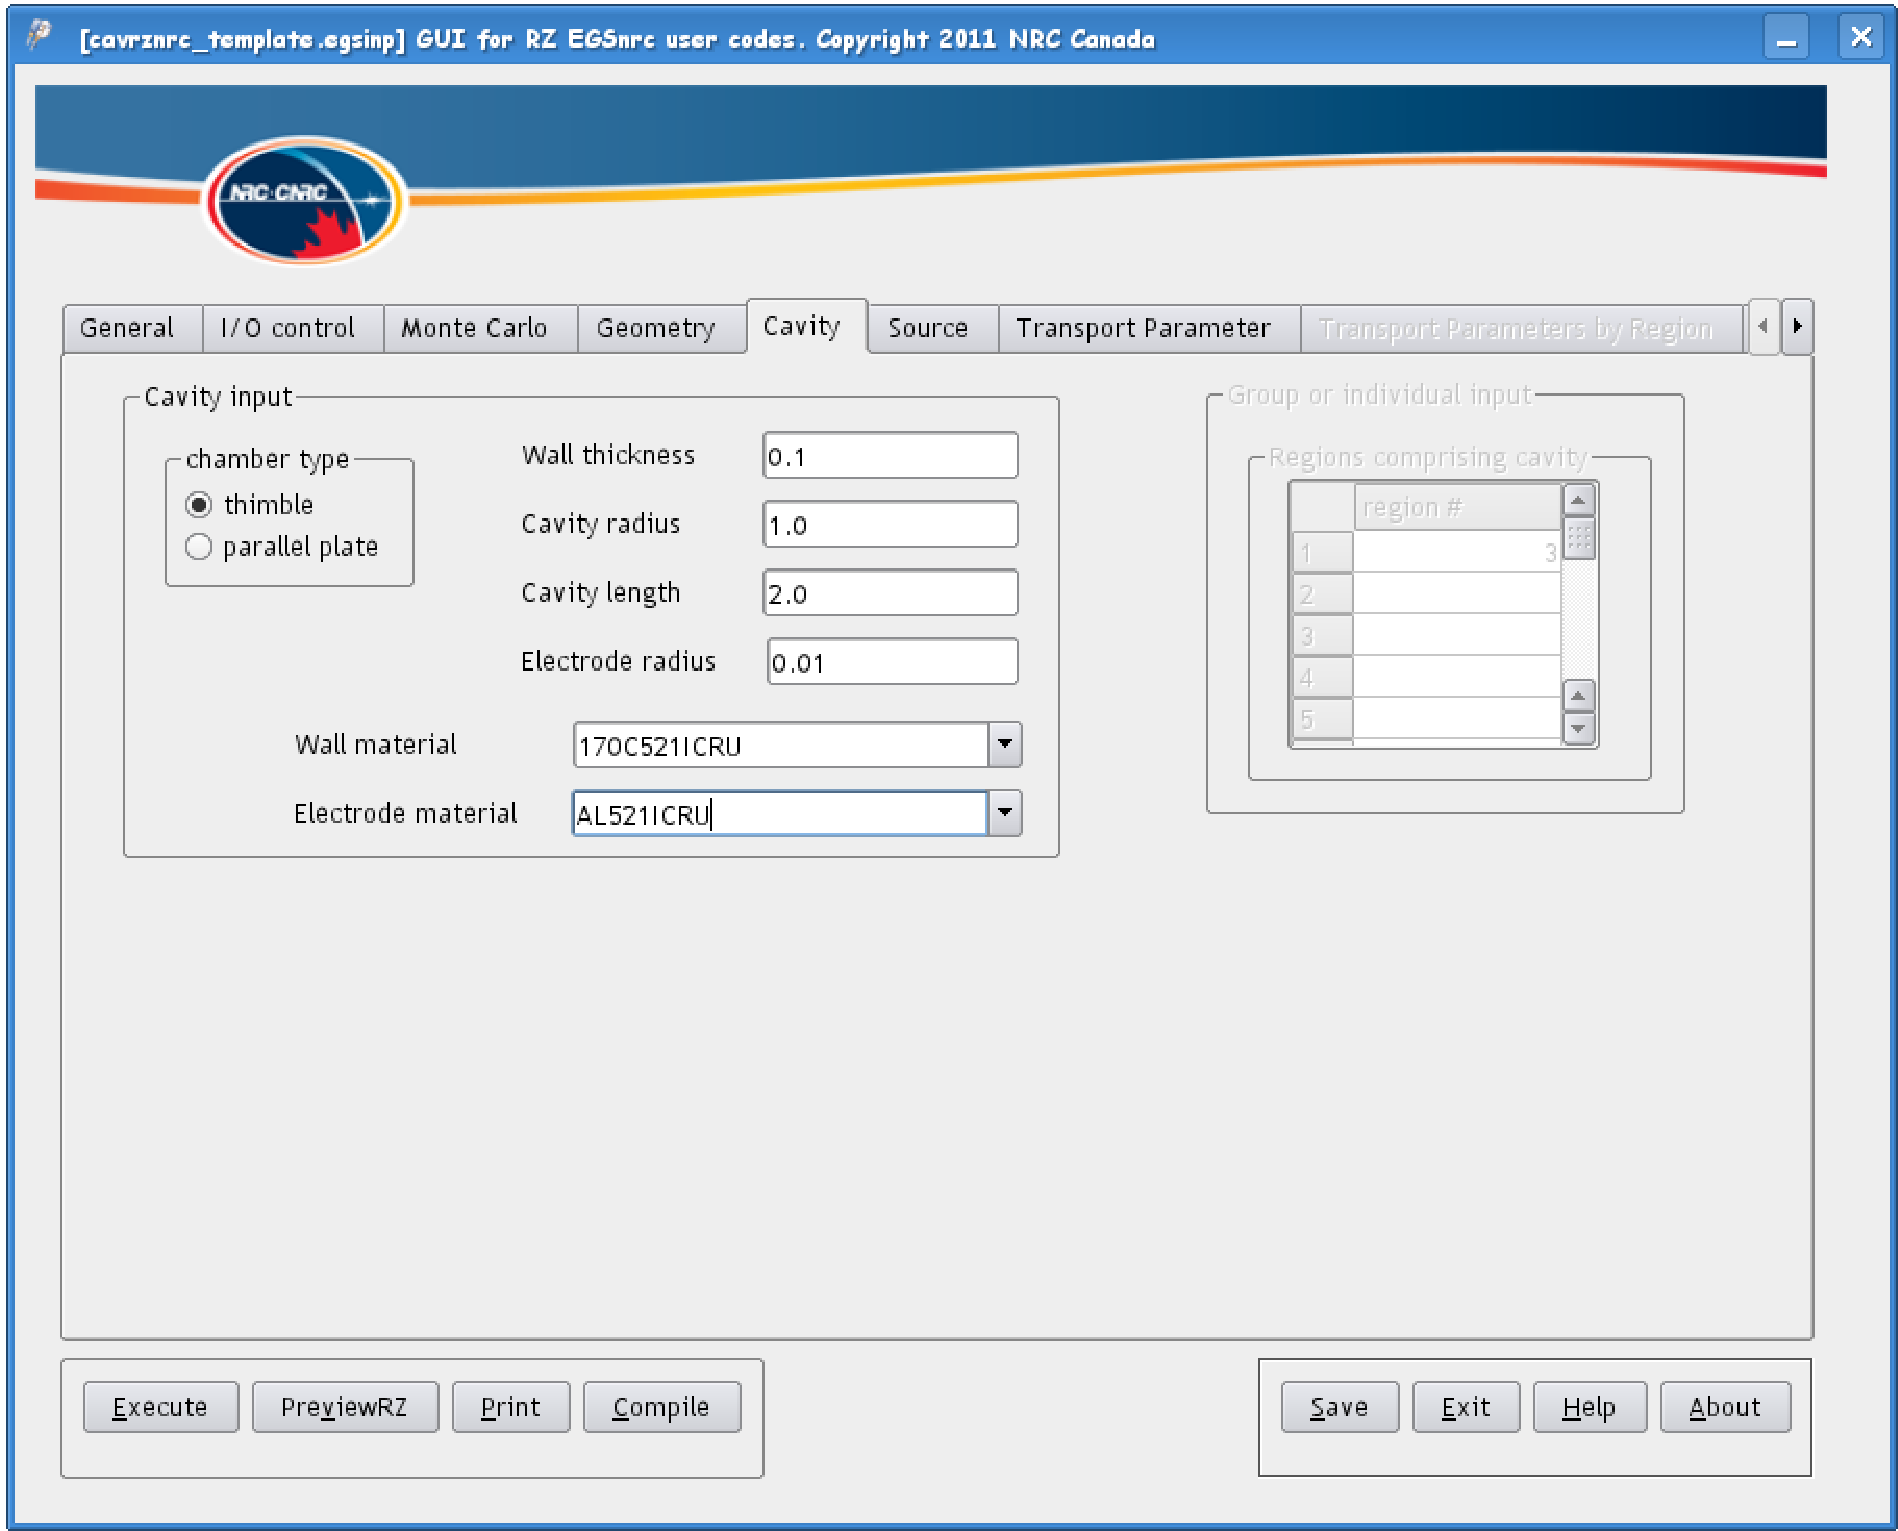
\includegraphics[height=11.56cm]{figures/cavity}
\end{center}
\end{latexonly}
\begin{center}

\includegraphics[height=1mm]{figures/fake2}
\end{center}
\caption{Cavity Input for the RZ EGSnrc User Code CAVRZnrc.}
\label{cavity_control}
\end{figure}

\clearpage
\newpage
\subsection{The Source Tab}
Any input related to the initial characteristics of the beam or phase space file are entered
here. There are 15 different types of source geometries that can be entered. A detailed description
of each source can be found in the NRC User Codes Manual (NRCC report PIRS-702\cite{Ro10})
and directly through the {\tt Tool Tips} help feature offered by this GUI. \\ \\

\begin{figure}[htb]
\begin{htmlonly}
\begin{rawhtml}
<p><center>
<img src="figures/src.png" name=srcfig><br><br>
</center>
\end{rawhtml}
\end{htmlonly}
\begin{latexonly}
\begin{center}
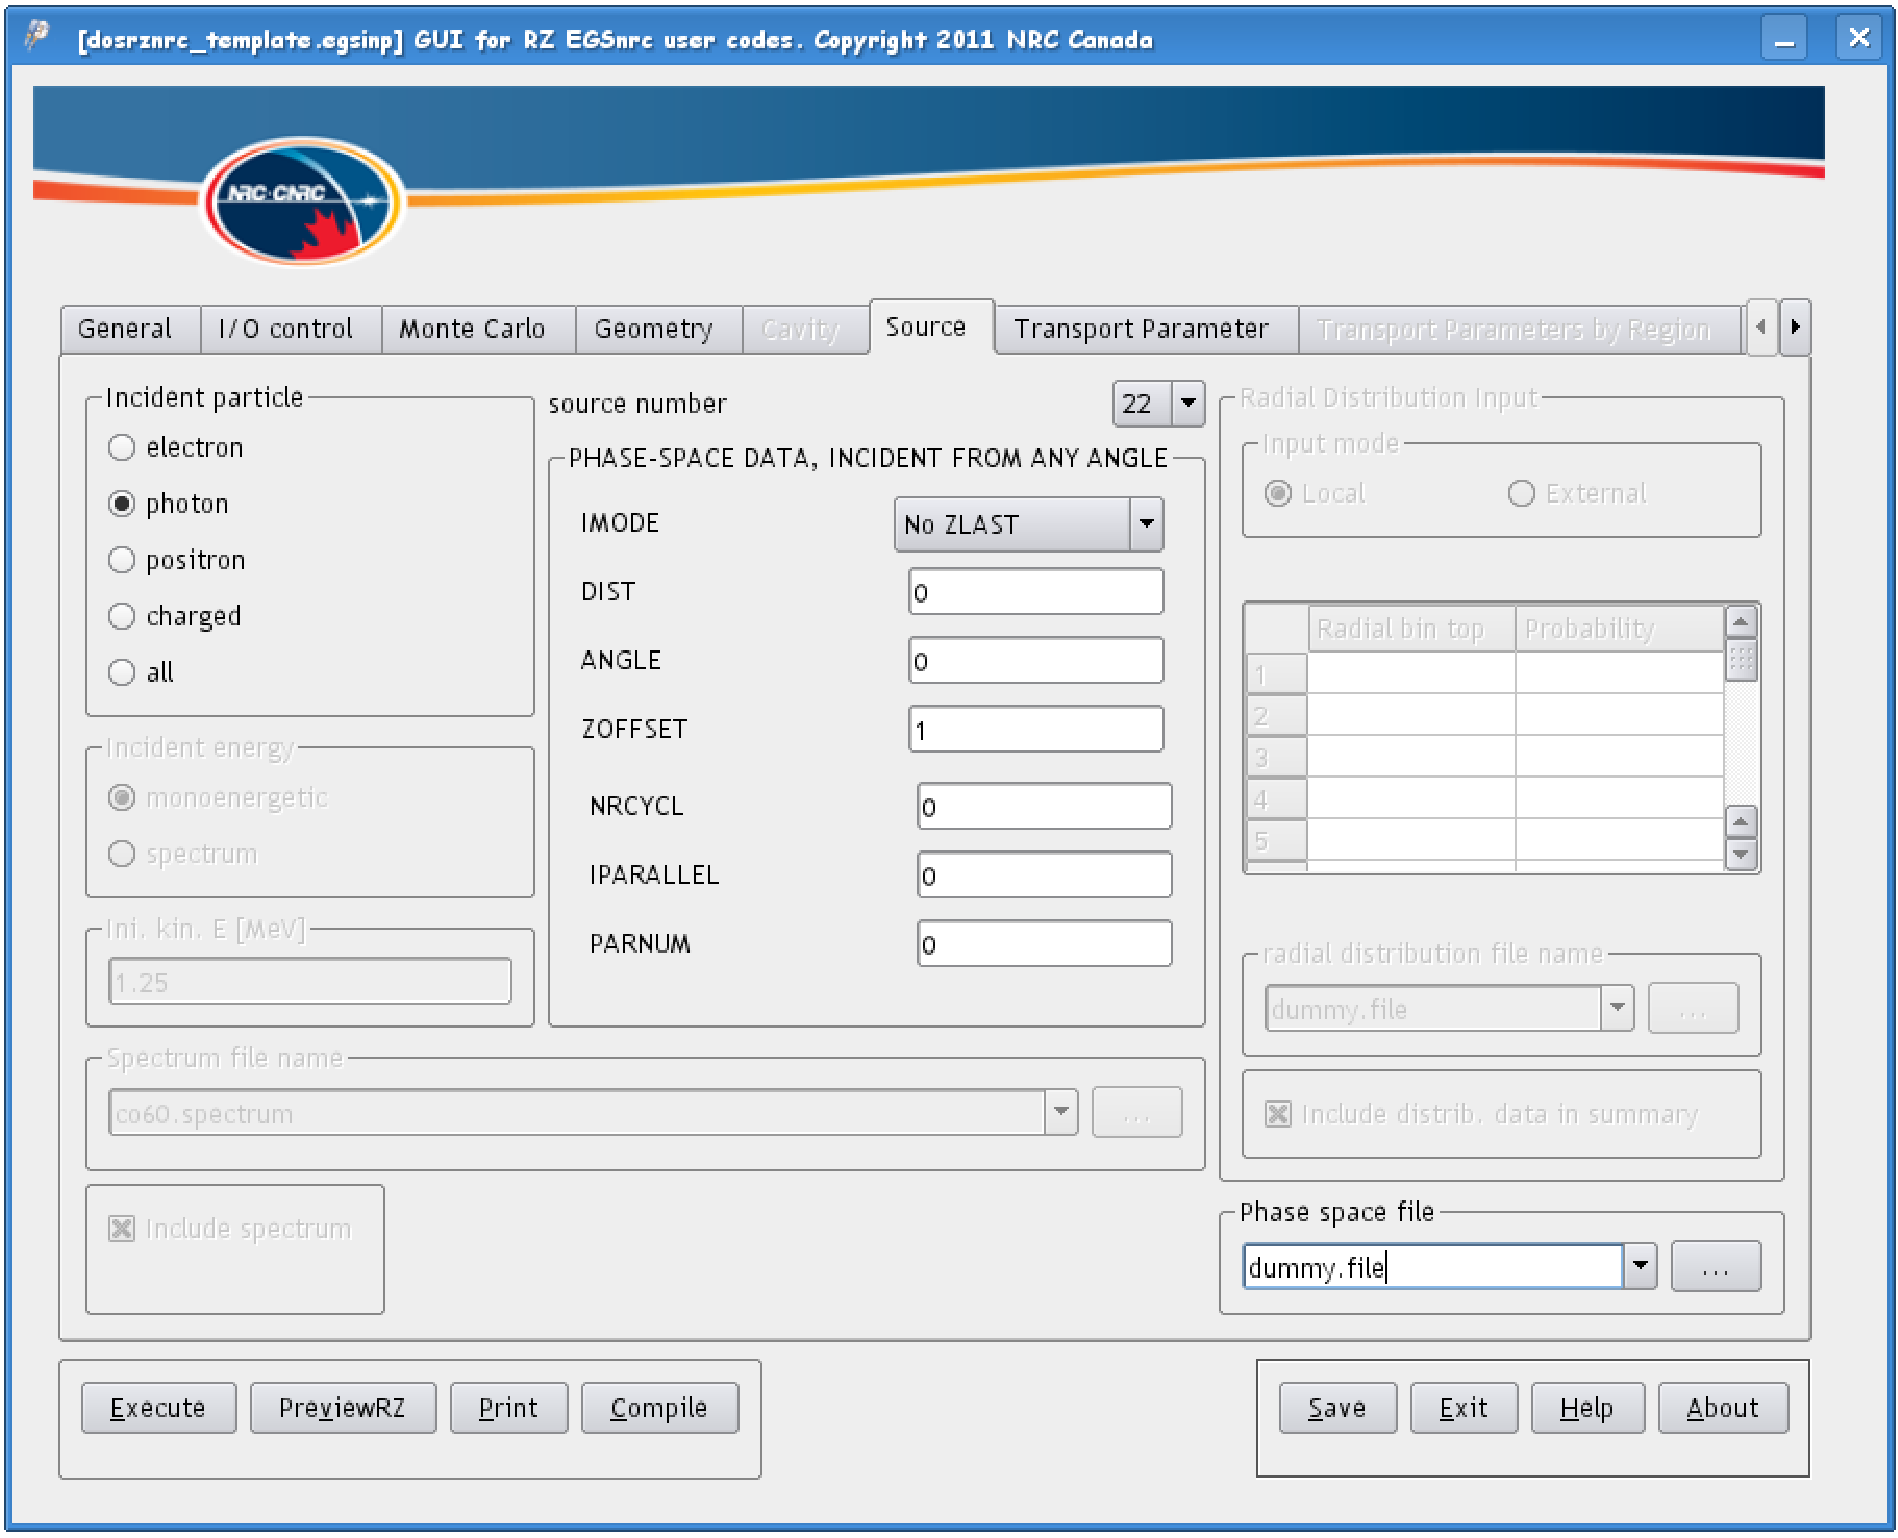
\includegraphics[height=11.56cm]{figures/src}
\end{center}
\end{latexonly}
\begin{center}

\includegraphics[height=1mm]{figures/fake2}
\end{center}
\caption{Source Input for the RZ EGSnrc User Codes.}
\label{srcfig}
\end{figure}

If the user selects source 21 or 22,
the Phase-space file edit line becomes
enabled and one can either type the name
of a phase-space file or one can use the Open File Dialog
to navigate throught the directories to get the desired file.
In the latter case, the path is stripped from the file name,
but it is still rembered and properly added to the file name
when saving the input file. Although EGSnrc accepts phase-space files
with arbitrary extensions, it is customary to use the *.egsphsp1
extension for regular phase-space files and *.IAEAphsp for phase-space
files using the IAEA format (in this latter case, the extension is improtant).
Although the default filter for searching for files uses these
extensions (see figure \ref{src22_dlg}), the All files (*) filter is still available.

\begin{figure}[htb]
\begin{htmlonly}
\begin{rawhtml}
<p><center>
<img src="figures/src_22_dlg.png" name=src22dlg><br><br>
</center>
\end{rawhtml}
\end{htmlonly}
\begin{latexonly}
\begin{center}
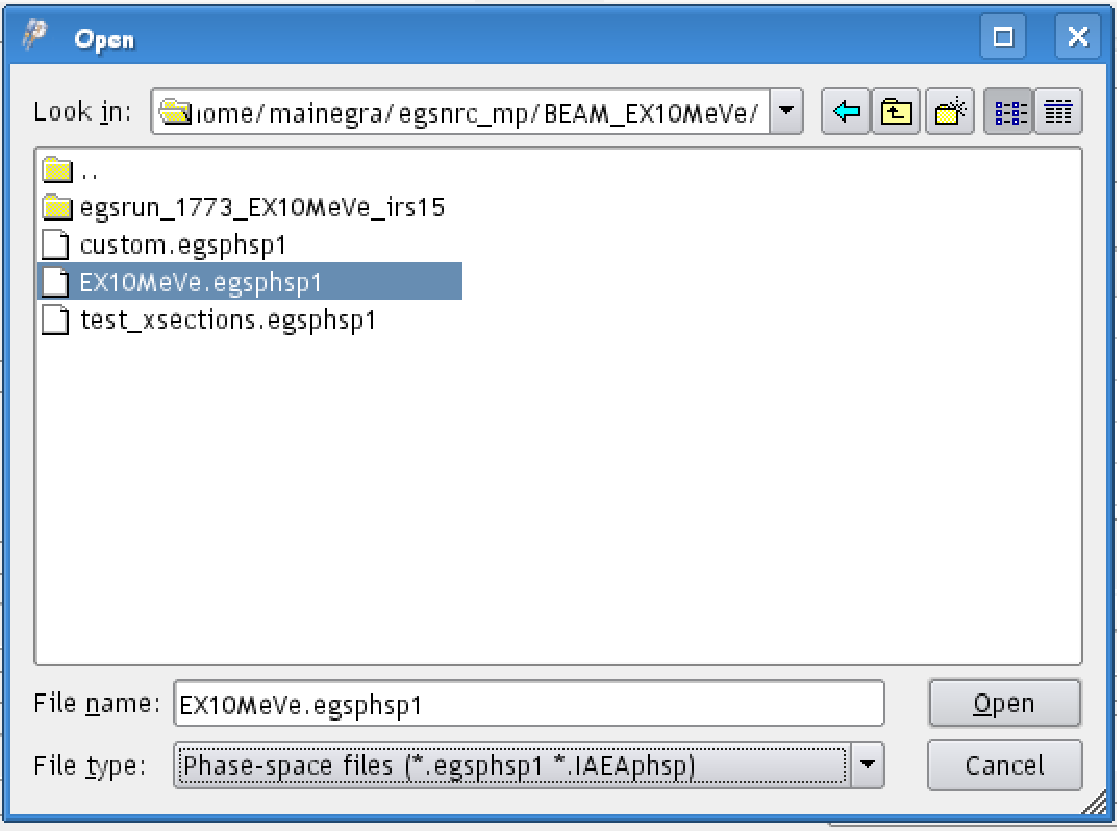
\includegraphics[height=10cm]{figures/src_22_dlg}
\end{center}
\end{latexonly}
\begin{center}

\includegraphics[height=1mm]{figures/fake2}
\end{center}
\caption{Phase-space open file dialog.}
\label{src22_dlg}
\end{figure}

\subsubsection{Setting up a BEAM Source}

Alternatively to phase-space files, EGSnrc can now use a
BEAMnrc simulation as a particle source (figure \ref{src23_fig}).
This source
(source 23) needs to be set up in a separate dialog. When
the user selects this source, a button appears with a red
text, prompting the user to enter the source parameters and
warning that unless there are BEAM user-codes compiled as
a library on the system, no BEAM user-code will be available.
\vspace*{5mm}

\begin{figure}[htb]
\begin{htmlonly}
\begin{rawhtml}
<p><center>
<img src="figures/src_23.png" name=srcfig><br><br>
</center>
\end{rawhtml}
\end{htmlonly}
\begin{latexonly}
\begin{center}
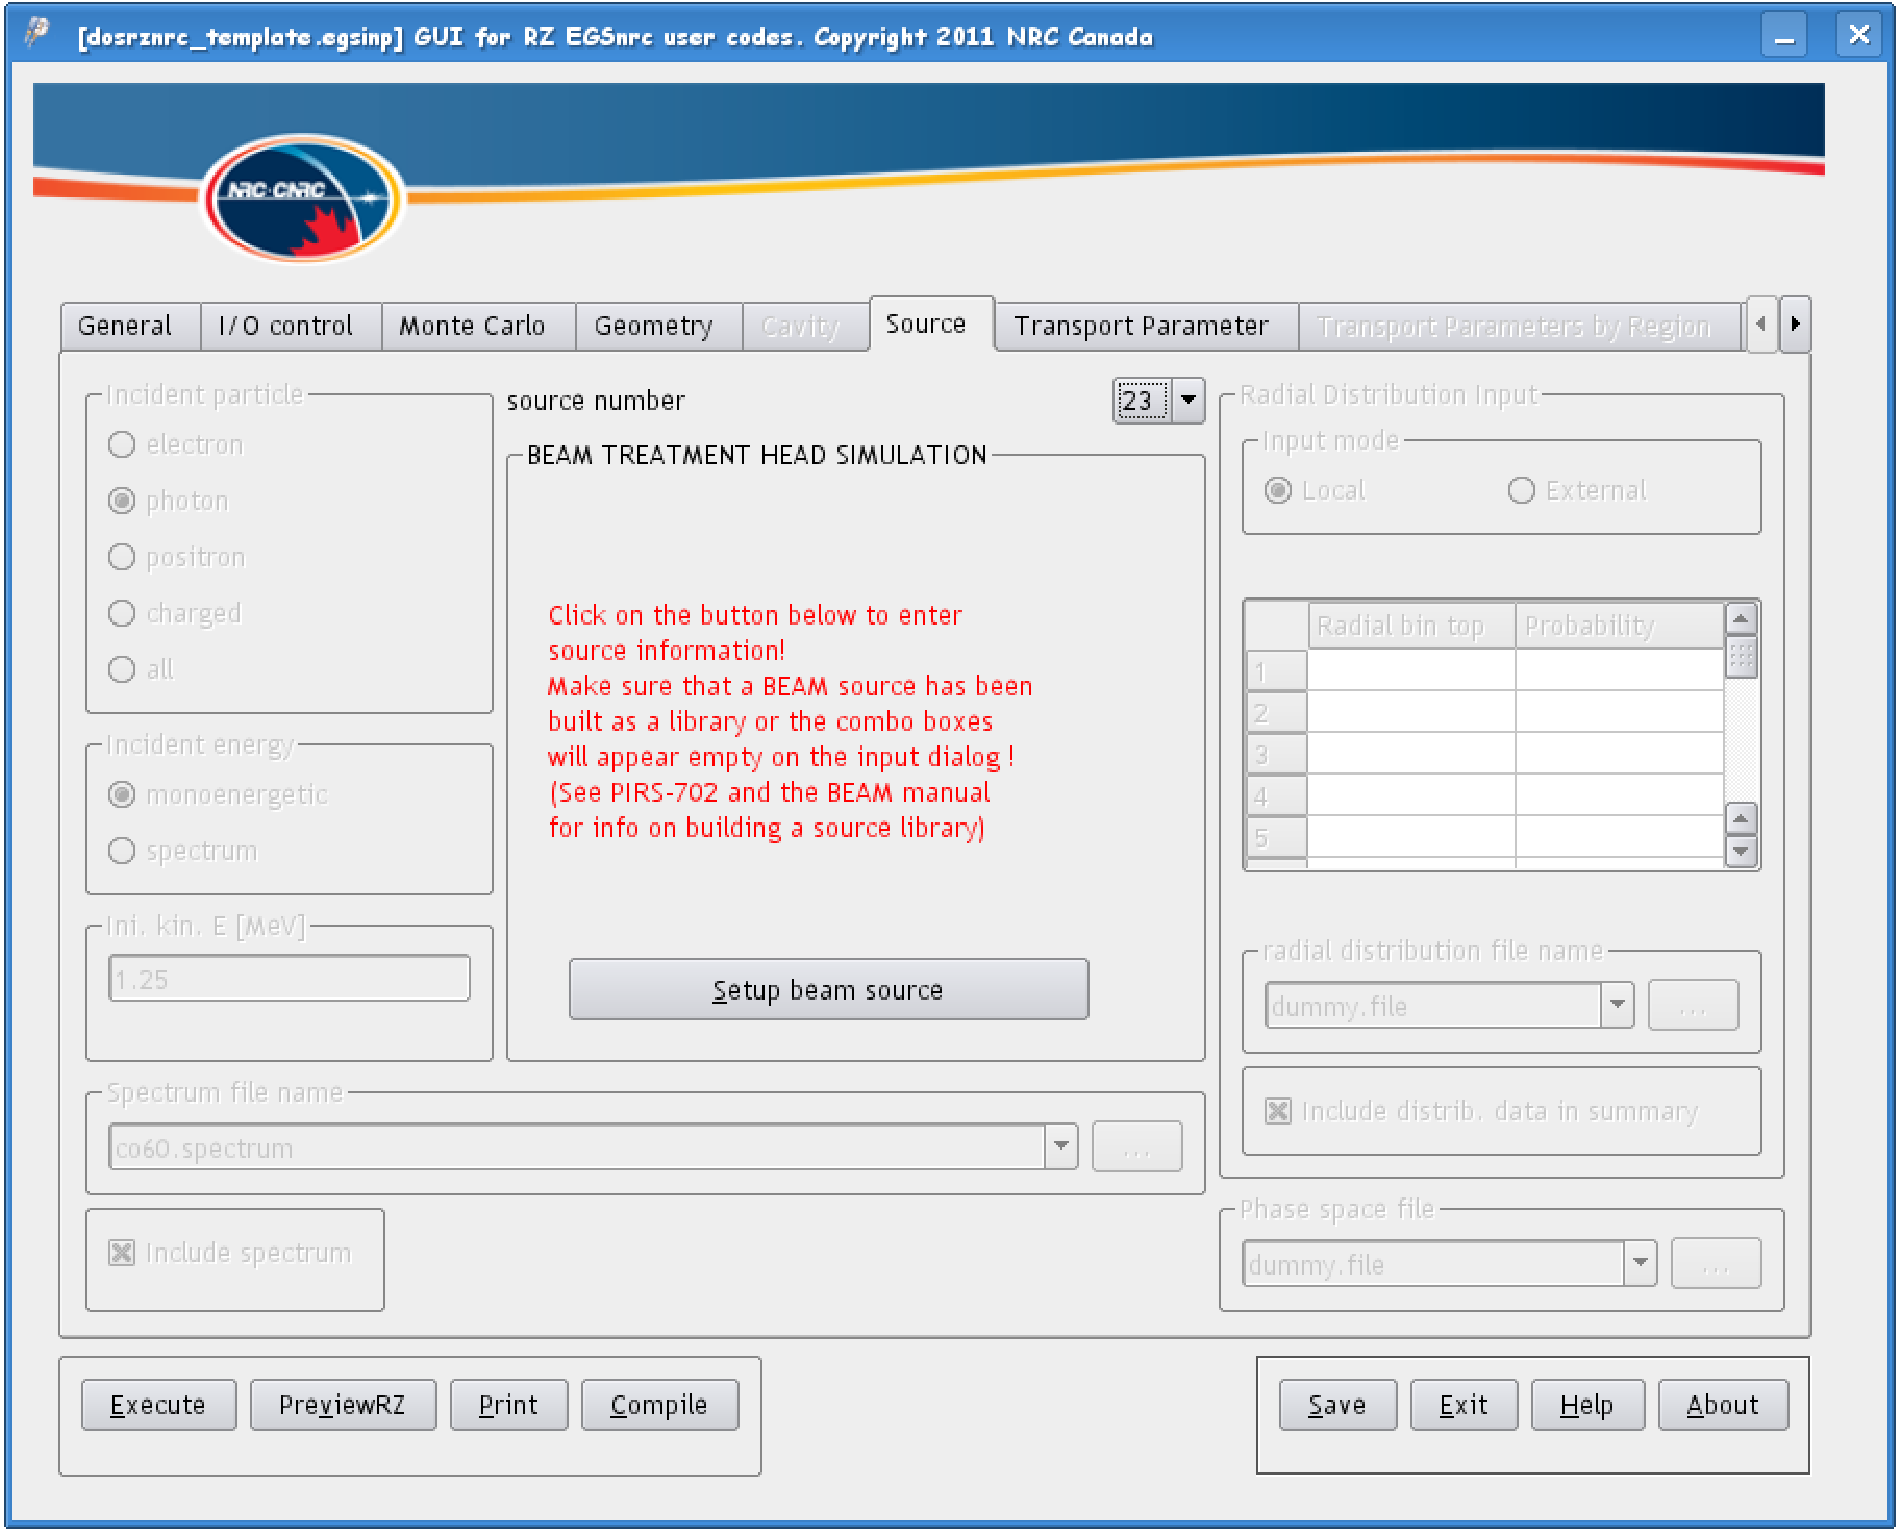
\includegraphics[height=11.56cm]{figures/src_23}
\end{center}
\end{latexonly}
\begin{center}

\includegraphics[height=1mm]{figures/fake2}
\end{center}
\caption{Selecting BEAMnrc as a source.}
\label{src23_fig}
\end{figure}

Clicking on the above mentioned button brings a new dialog (figure \ref{src23_dlg}),
where the user can enter the name of the BEAM user-code, the BEAM
input file and the required PEGS4 data file based on the current
PEGS4 directory. The user can also define a weight window
for the particles and the positioning and orientation of the
source.

\begin{figure}[htb]
\begin{htmlonly}
\begin{rawhtml}
<p><center>
<img src="figures/src_23_dlg.png" name=src23dlg><br><br>
</center>
\end{rawhtml}
\end{htmlonly}
\begin{latexonly}
\begin{center}
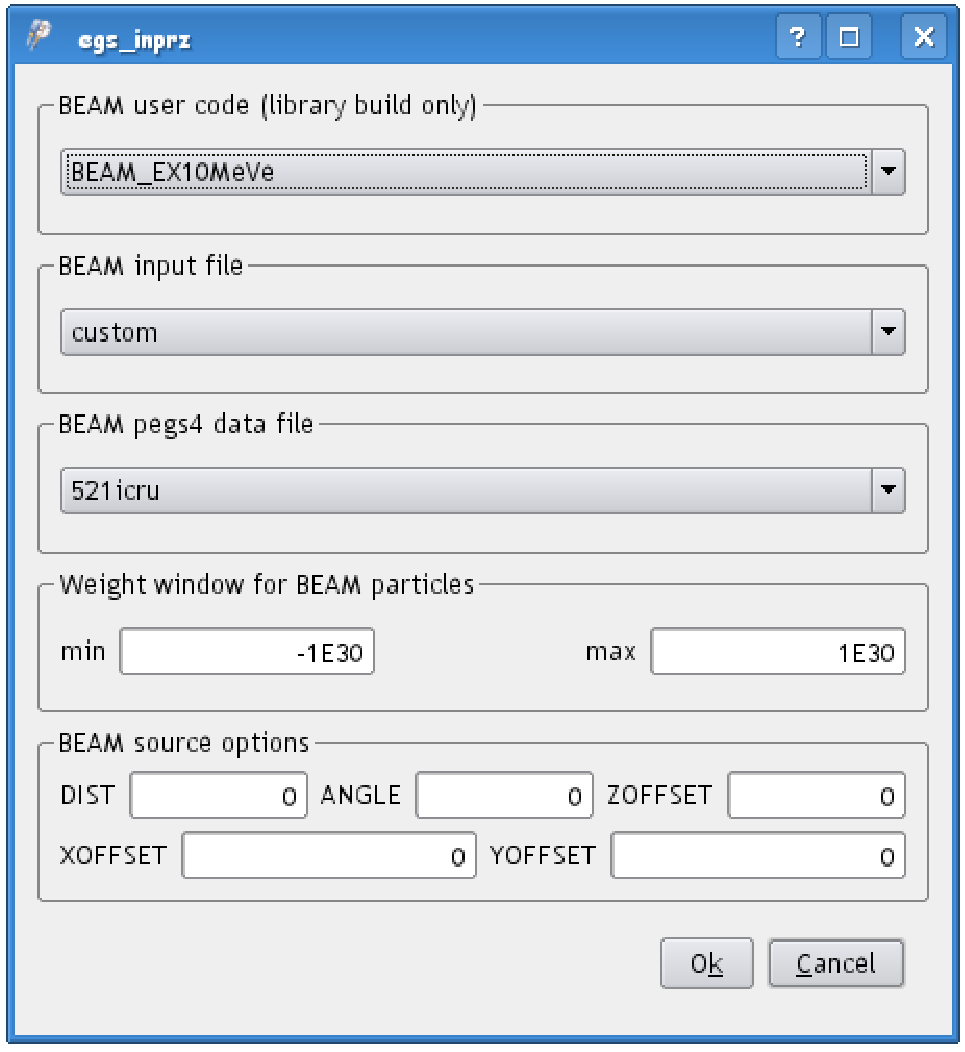
\includegraphics[height=10cm]{figures/src_23_dlg}
\end{center}
\end{latexonly}
\begin{center}

\includegraphics[height=1mm]{figures/fake2}
\end{center}
\caption{BEAMnrc source definition dialog.}
\label{src23_dlg}
\end{figure}

\clearpage
% \newpage
\subsection{The Transport Parameters Tab}

This input section gathers information inherent to the physics of the transport of electromagnetic
radiation through matter. Threshold energies for photons and electrons, electron transport algorithm
to be used, as well as the cross section data and angular distributions to be used are entries that
are defined here. By default, EGSnrc uses threshold energies given by AP and AE in each region
for photons and electrons respectively. The electron transport is originally set to the EGSnrc default
algorithm, which is independent of electron step size. The user can also choose to turn {\em on}
and {\em off} other effects in the simulation, like Compton binding effects, spin effects, Rayleigh
scattering, atomic relaxations and angular sampling of the photo-electrons. For a detailed
reading on the physics of the transport of photons and electrons the user is refered to the
EGSnrc system manual (NRCC Report PIRS-701\cite{Ka09a}).\\

\begin{figure}[htb]
\begin{htmlonly}
\begin{rawhtml}
<p><center>
<img src="figures/mct.png" name=mctfig><br><br>
</center>
\end{rawhtml}
\end{htmlonly}
\begin{latexonly}
\begin{center}
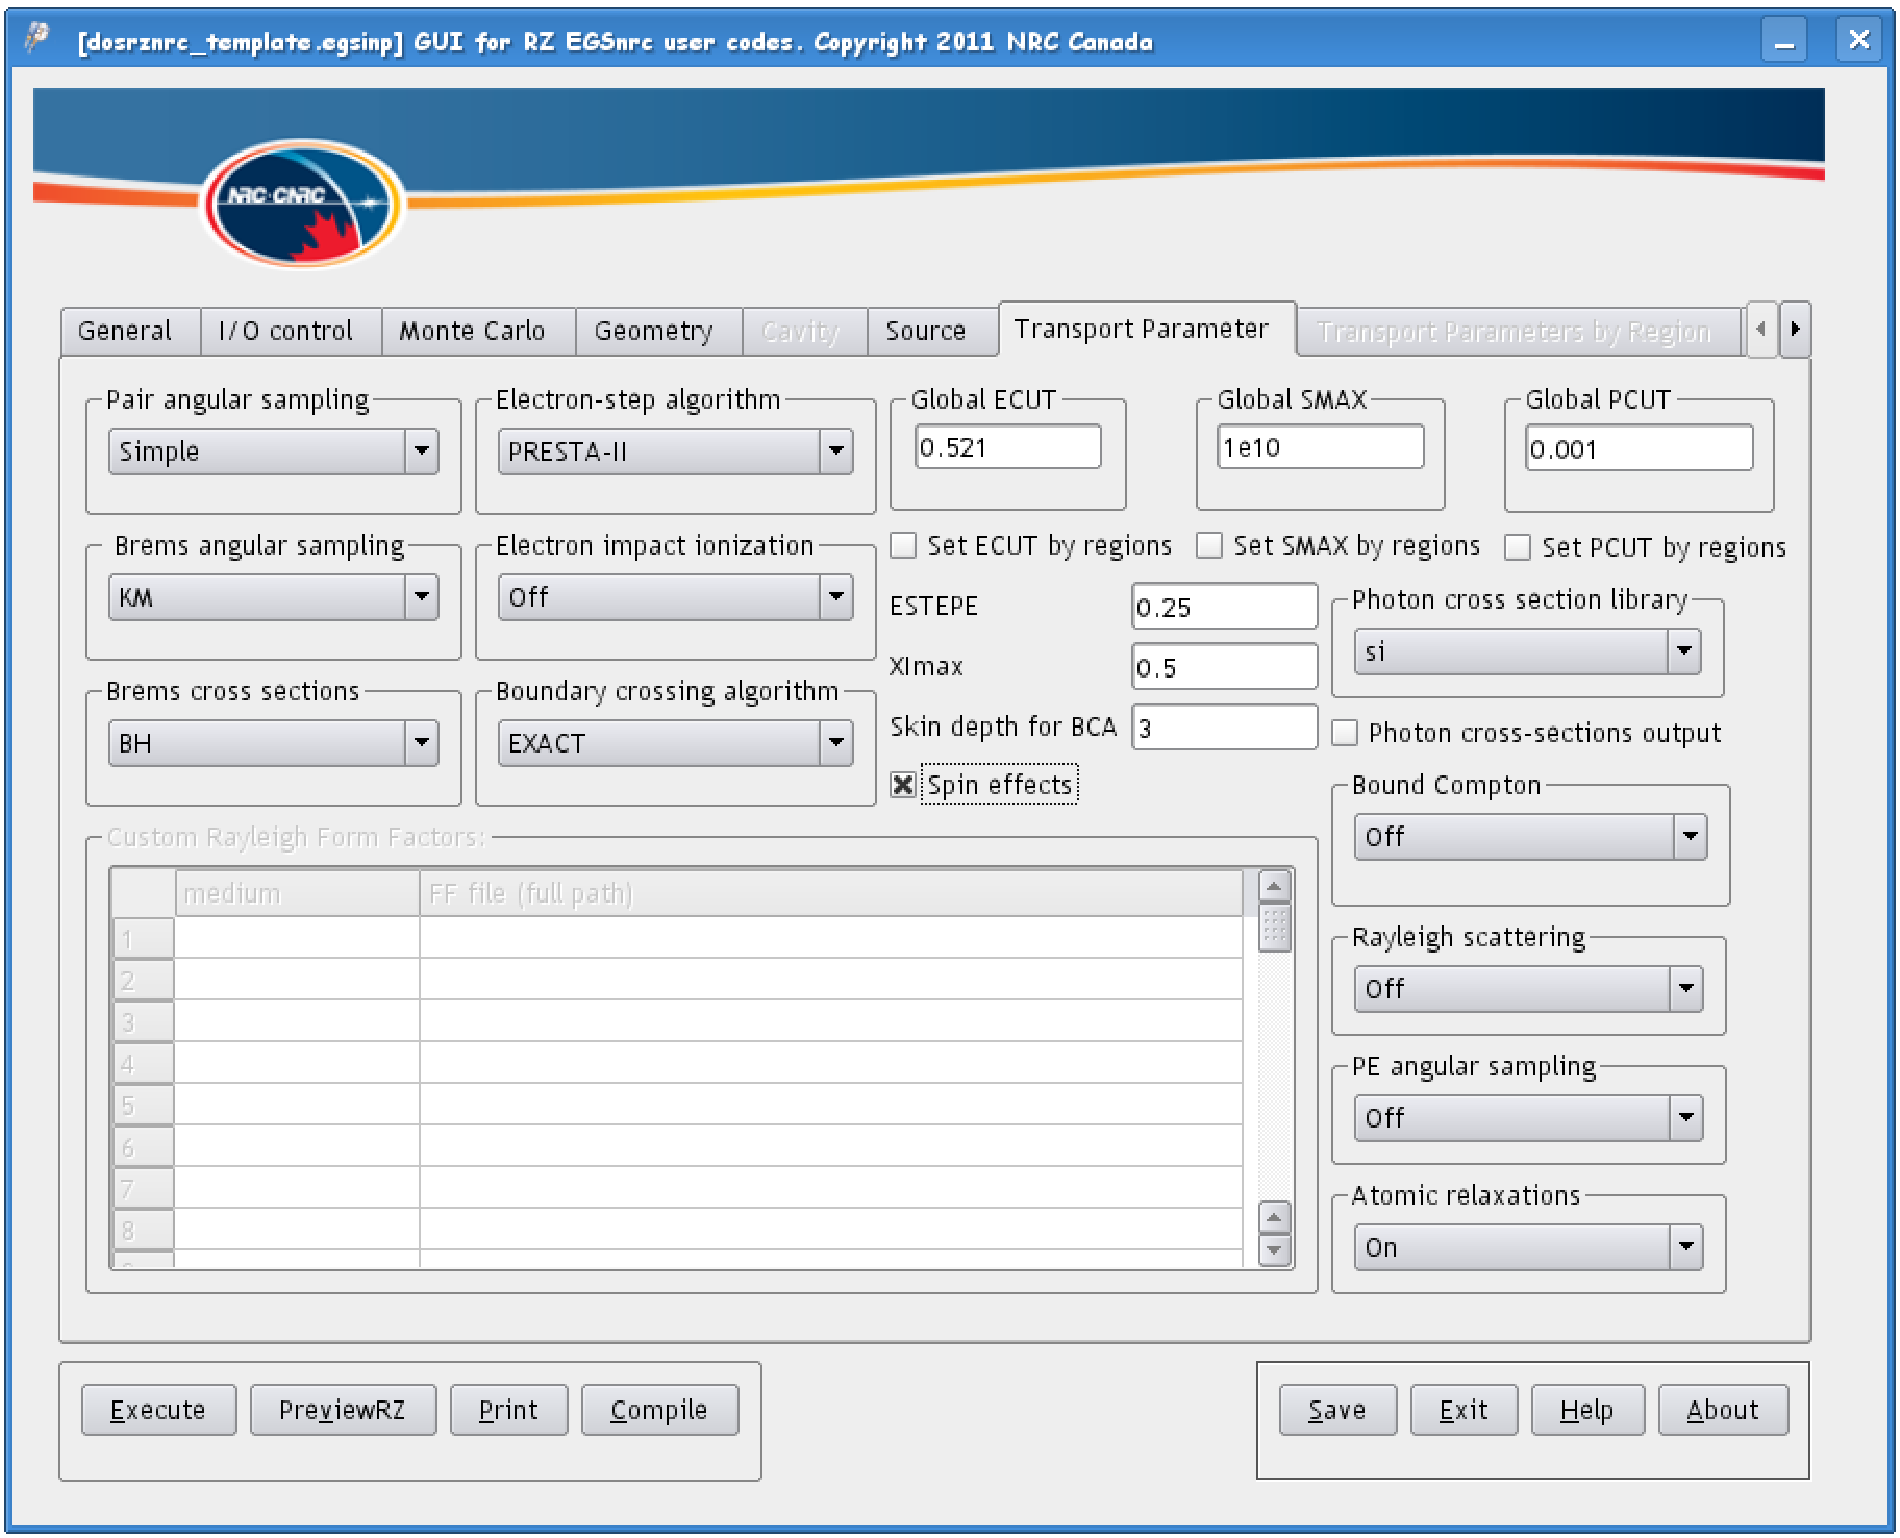
\includegraphics[height=11.56cm]{figures/mct}
\end{center}
\end{latexonly}
\begin{center}

\includegraphics[height=1mm]{figures/fake2}
\end{center}
\caption{Monte Carlo Transport Parameter Input for the RZ EGSnrc User Codes.}
\label{mctfig}
\end{figure}

This tab has been updated to most of the latest additions to the {\tt MC trasport parameters}
input block. Notably, one can now enter the medium and file names for using custom coherent
scattering form factors. Currently the option for defining an arbitrary file with Compton
cross sections is not available in the GUI. This wizard tab is already overloaded and will
be split in individual tabs for photon and electron/positron inputs in future releases.

\newpage
\subsection{The Transport Parameters by Regions Tab}

For some applications it might be desirable to have some of the quantities defined on a region by
region basis. This can be done by checking the corresponding check box or radio button of the quantity
chosen in the {\em Transport Parameter} tab. As soon as the user selects a quantity to be set by region
this tab is enabled. Here are tables for each of the quantities than can be set up on a region by region
basis. Tables will {\em only} be enabled for those quantities selected in the previous tab. \\ \\

\begin{figure}[htb]
\begin{htmlonly}
\begin{rawhtml}
<p><center>
<img src="figures/mctpr.png" name=mctprfig><br><br>
</center>
\end{rawhtml}
\end{htmlonly}
\begin{latexonly}
\begin{center}
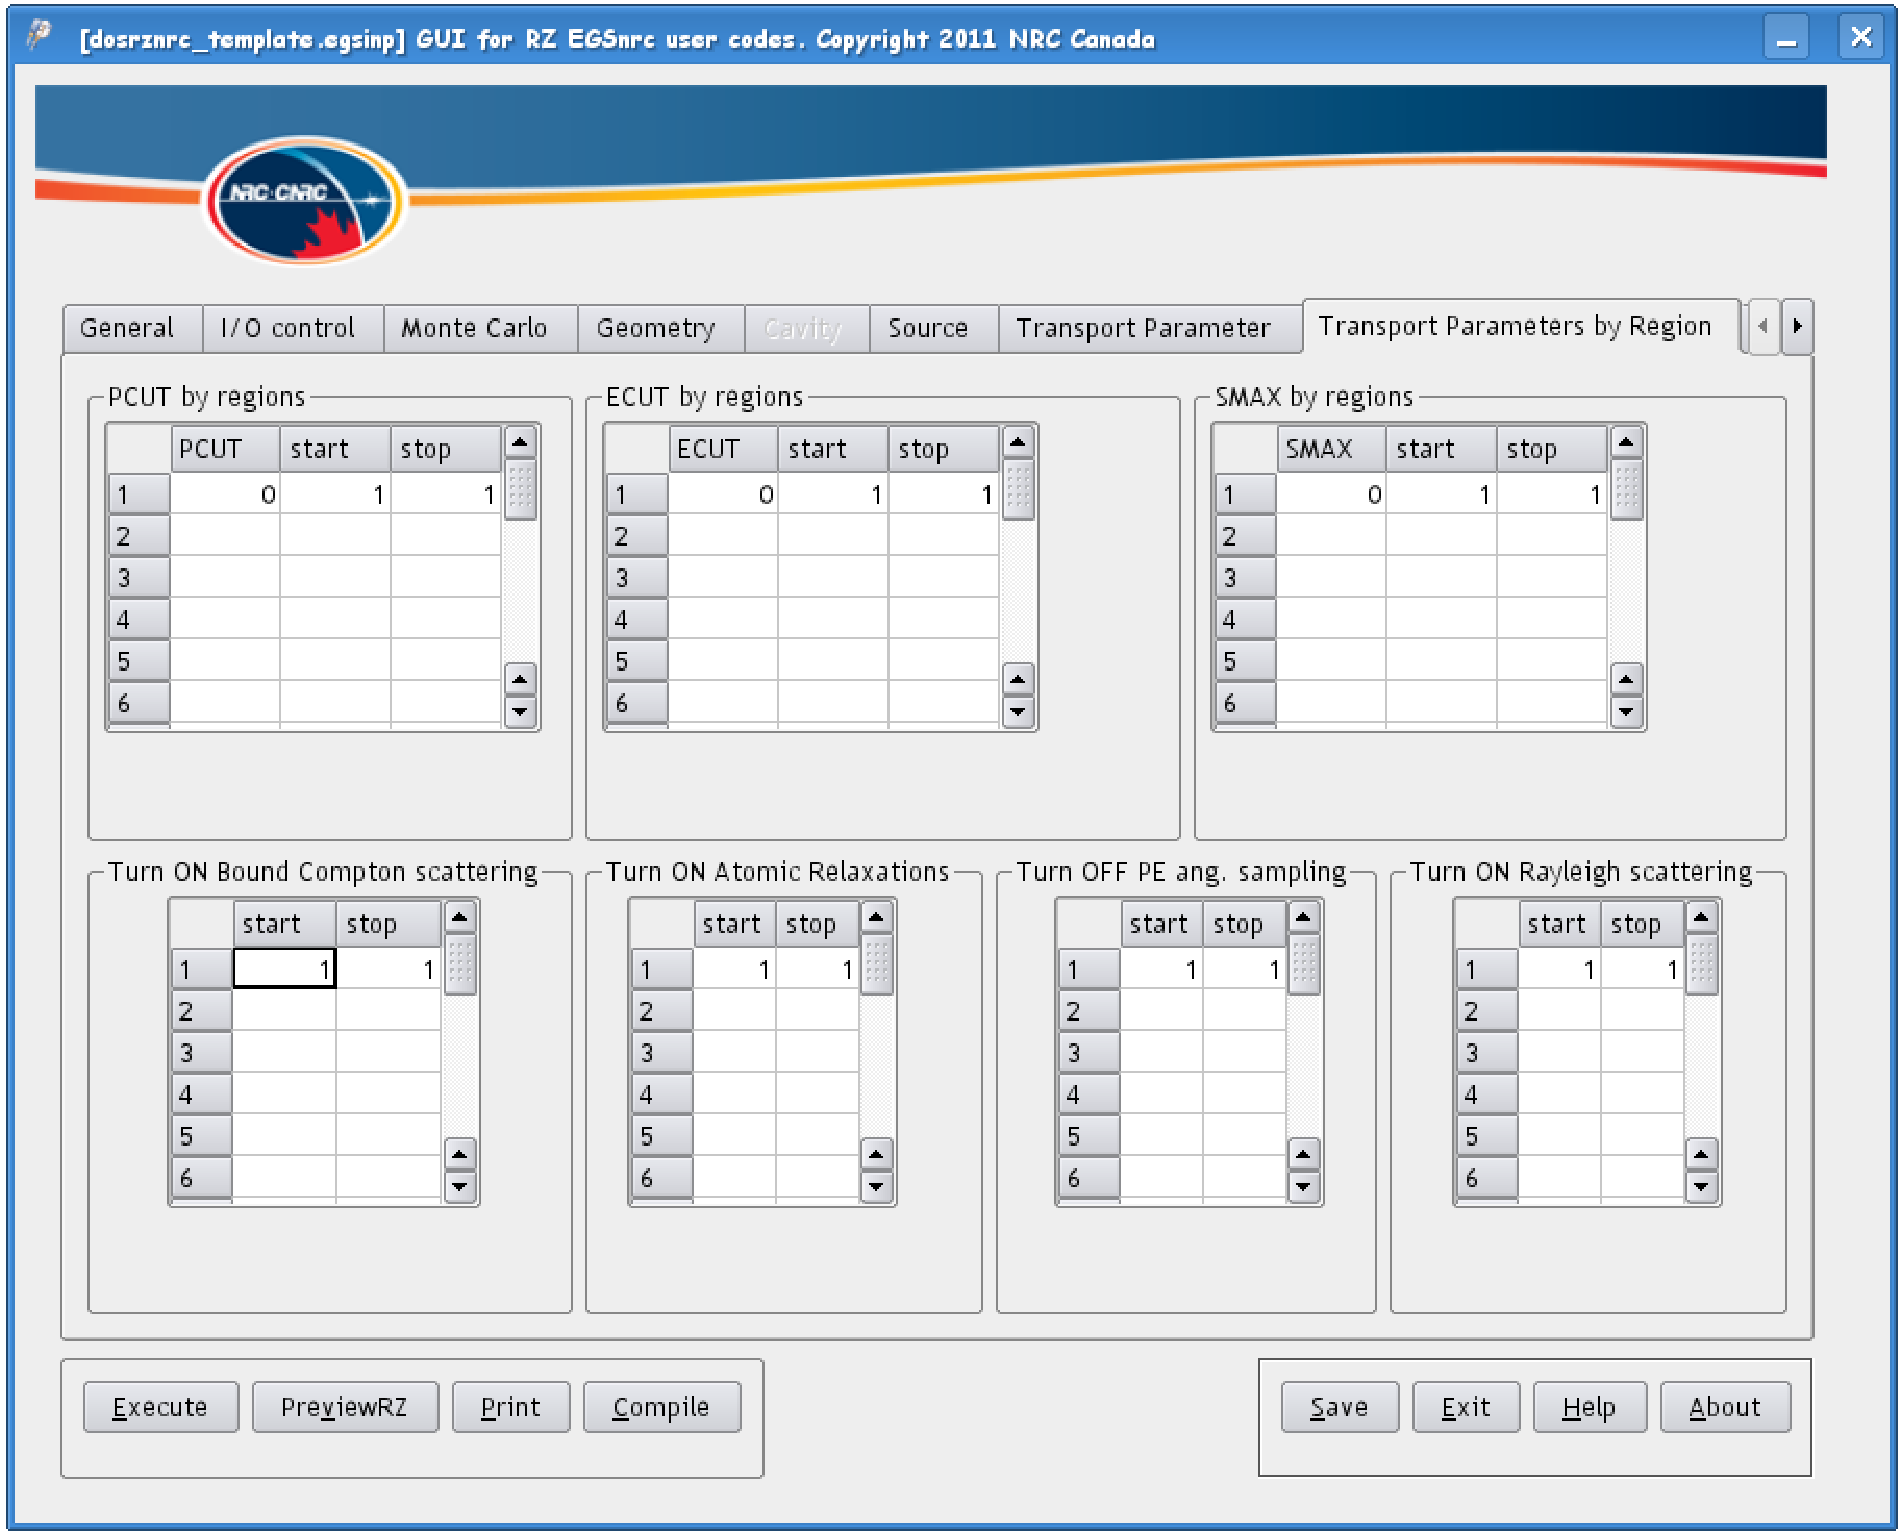
\includegraphics[height=11.56cm]{figures/mctpr}
\end{center}
\end{latexonly}
\begin{center}

\includegraphics[height=1mm]{figures/fake2}
\end{center}
\caption{Transport Parameter per Regions Input for the RZ EGSnrc User Codes.}
\label{mctprfig}
\end{figure}

\newpage
\subsection{The Variance Reduction Tab}

In this tab the user can define the parameters for the different variance reduction techniques
incorporated in the specific user-codes. Techniques like electron range rejection,
bremsstrahlung splitting and Russian Roulette are now implemented in EGSnrc. Pathlength biasing and
photon forcing are implemented in all user-codes except FLURZnrc, which only includes photon
forcing. Additionally photon cross section enhancement is available in DOSRZnrc
and CAVRZnrc and a photon splitting technique is also available in CAVRZnrc.
See the NRC User Codes Manual for information on these techniques (NRCC report PIRS-702\cite{Ro10}).
\\ \\

\begin{figure}[htb]
\begin{htmlonly}
\begin{rawhtml}
<p><center>
<img src="figures/var.png" name=varfig><br><br>
</center>
\end{rawhtml}
\end{htmlonly}
\begin{latexonly}
\begin{center}
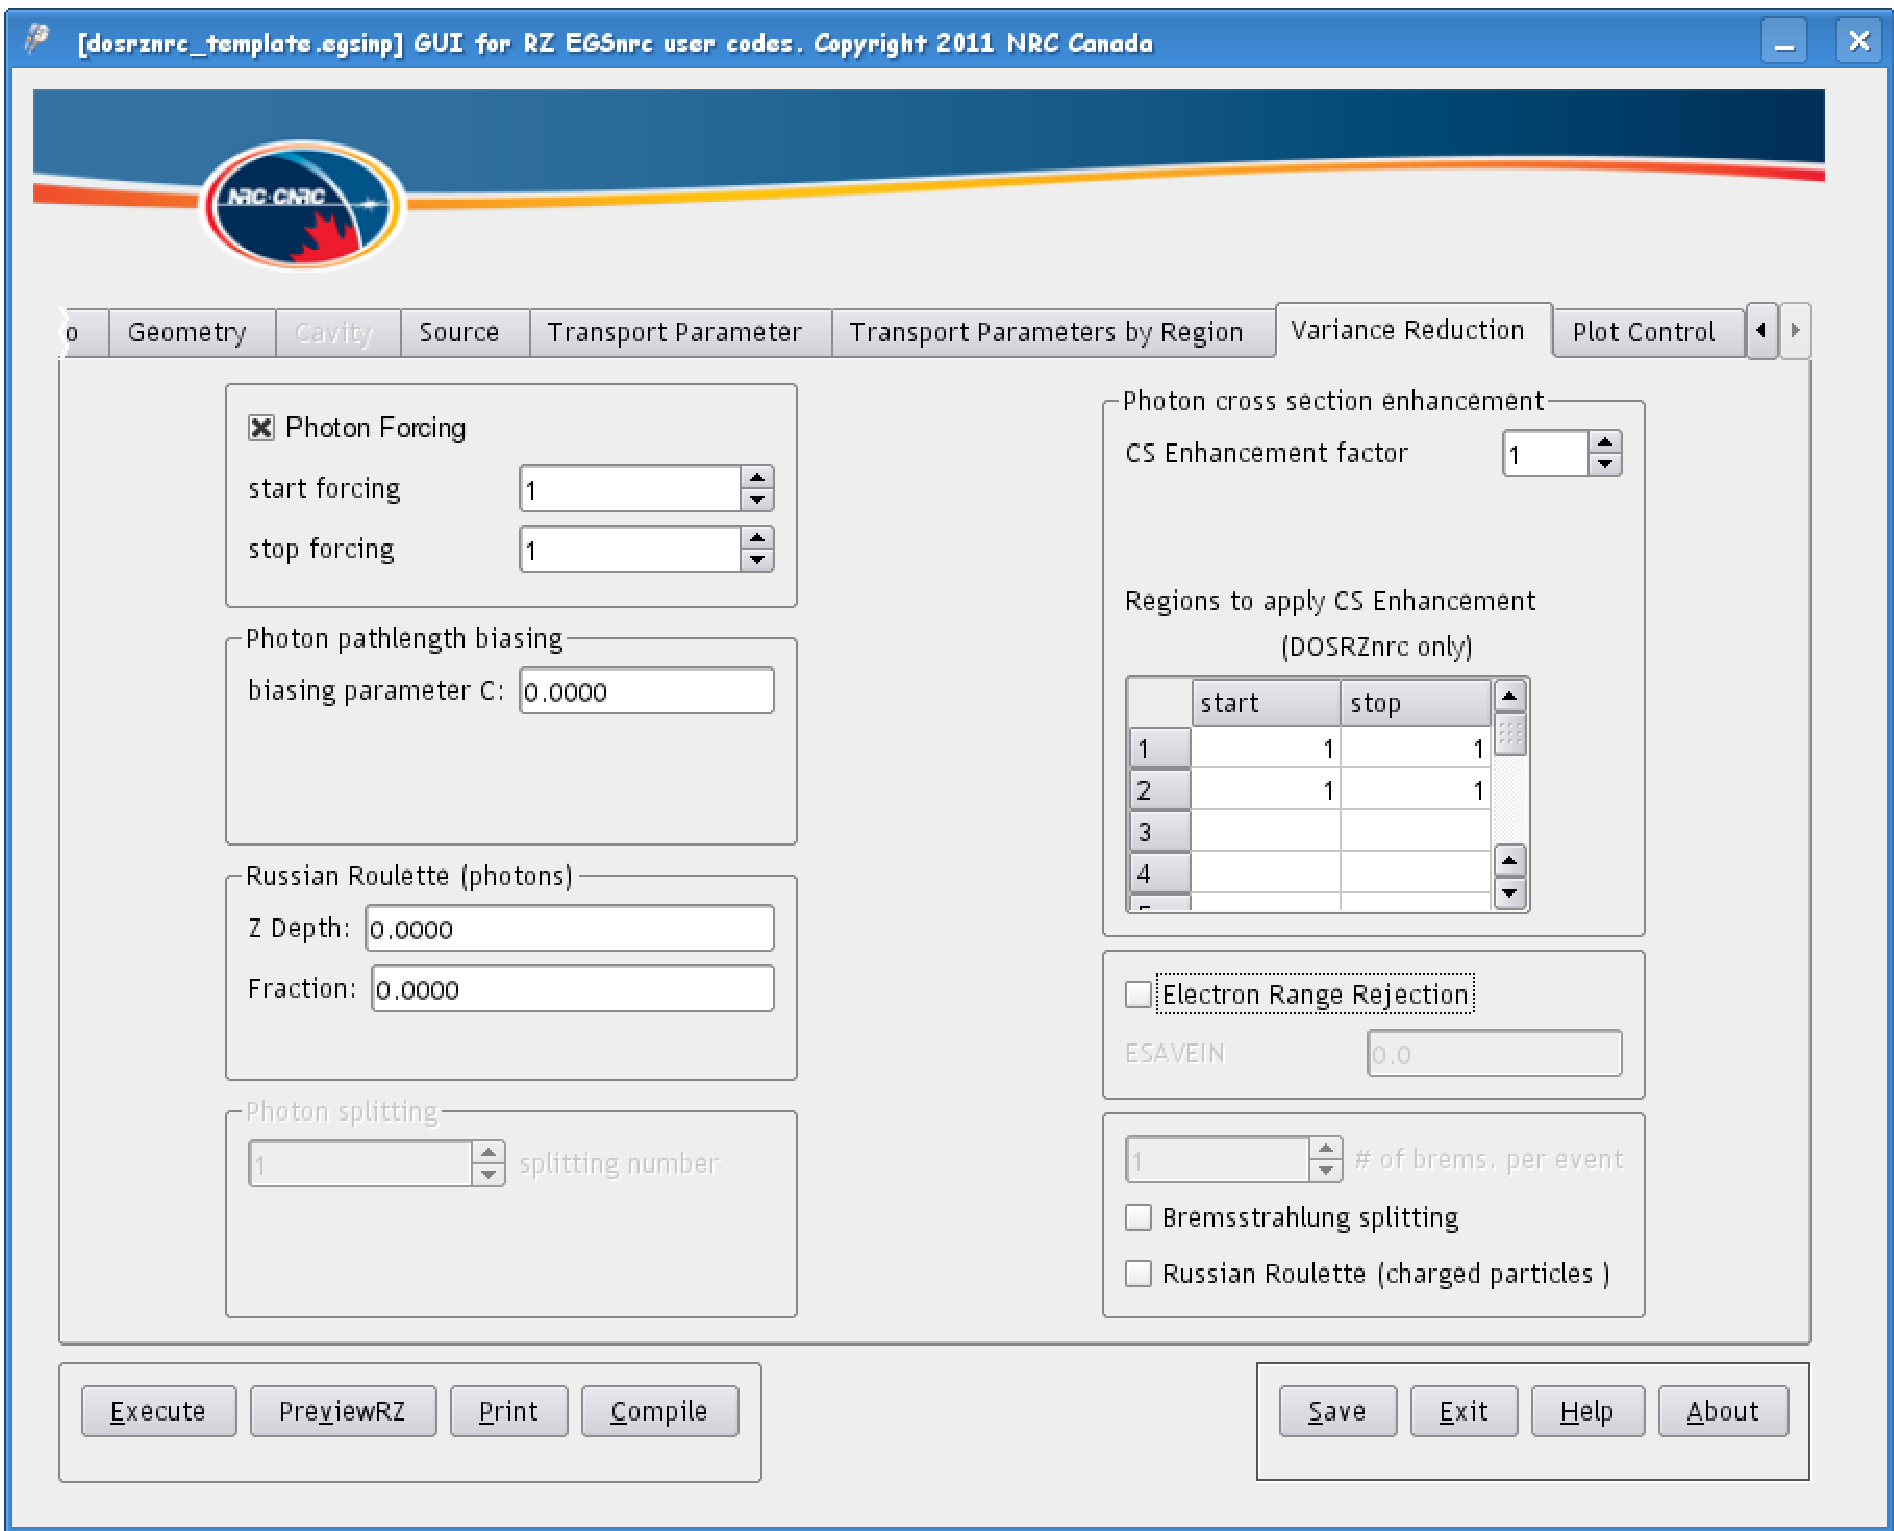
\includegraphics[height=11.56cm]{figures/var}
\end{center}
\end{latexonly}
\begin{center}

\includegraphics[height=1mm]{figures/fake2}
\end{center}
\caption{Variance Reduction Parameters for the RZ EGSnrc User Codes.}
\label{varfig}
\end{figure}

\newpage
\subsection{The Plot Control Tab}

This input block is only relevant for two of the user codes, DOSRZnrc and FLURZnrc.
DOSRZnrc has a section of inputs to control plotting of dose {\em vs} depth/radius results
(see figure \ref{plotdosrz}).
\begin{figure}[htb]
\begin{htmlonly}
\begin{rawhtml}
<p><center>
<img src="figures/plot_dosrz.png" name=plotdosrz><br><br>
</center>
\end{rawhtml}
\end{htmlonly}
\begin{latexonly}
\begin{center}
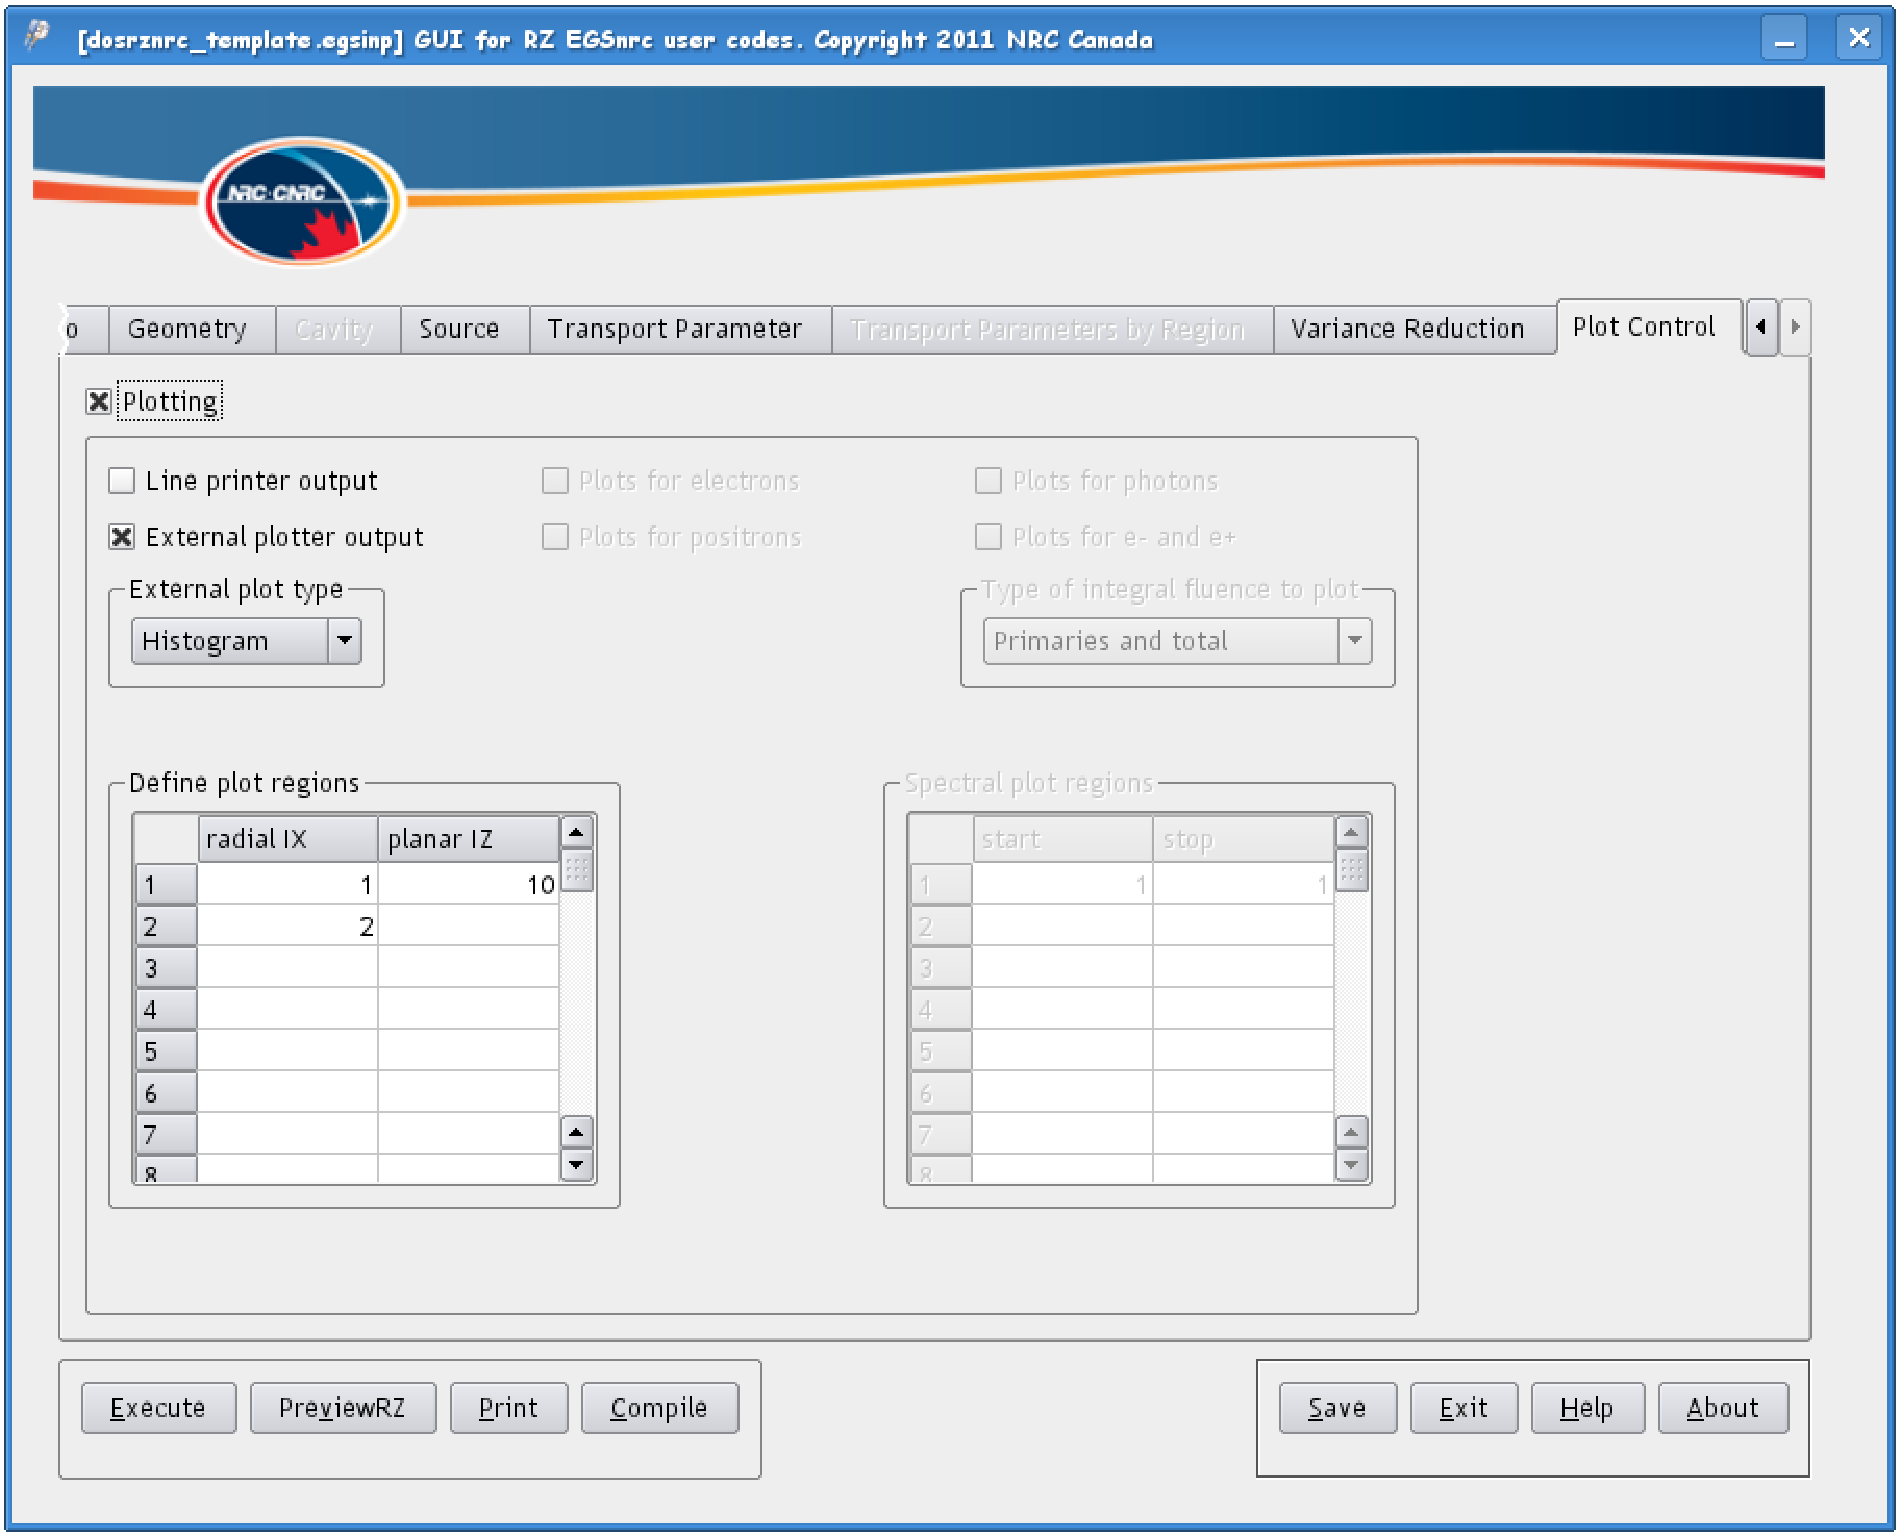
\includegraphics[height=11.56cm]{figures/plot_dosrz}
\end{center}
\end{latexonly}
\begin{center}

\includegraphics[height=1mm]{figures/fake2}
\end{center}
\caption{Plot Inputs for the RZ EGSnrc User Code DOSRZnrc.}
\label{plotdosrz}
\end{figure}

FLURZnrc has two distinct types of plotting outputs. One class of plots gives integral fluence {\em vs}
position plots in various ways ({\em vs} depth, {\em vs} radius). The code also ouputs fluence spectra
in specified regions (see figure \ref{plotflurz}).
\begin{figure}[htb]
\begin{htmlonly}
\begin{rawhtml}
<p><center>
<img src="figures/plot_flurz.png" name=plotflurz><br><br>
</center>
\end{rawhtml}
\end{htmlonly}
\begin{latexonly}
\begin{center}
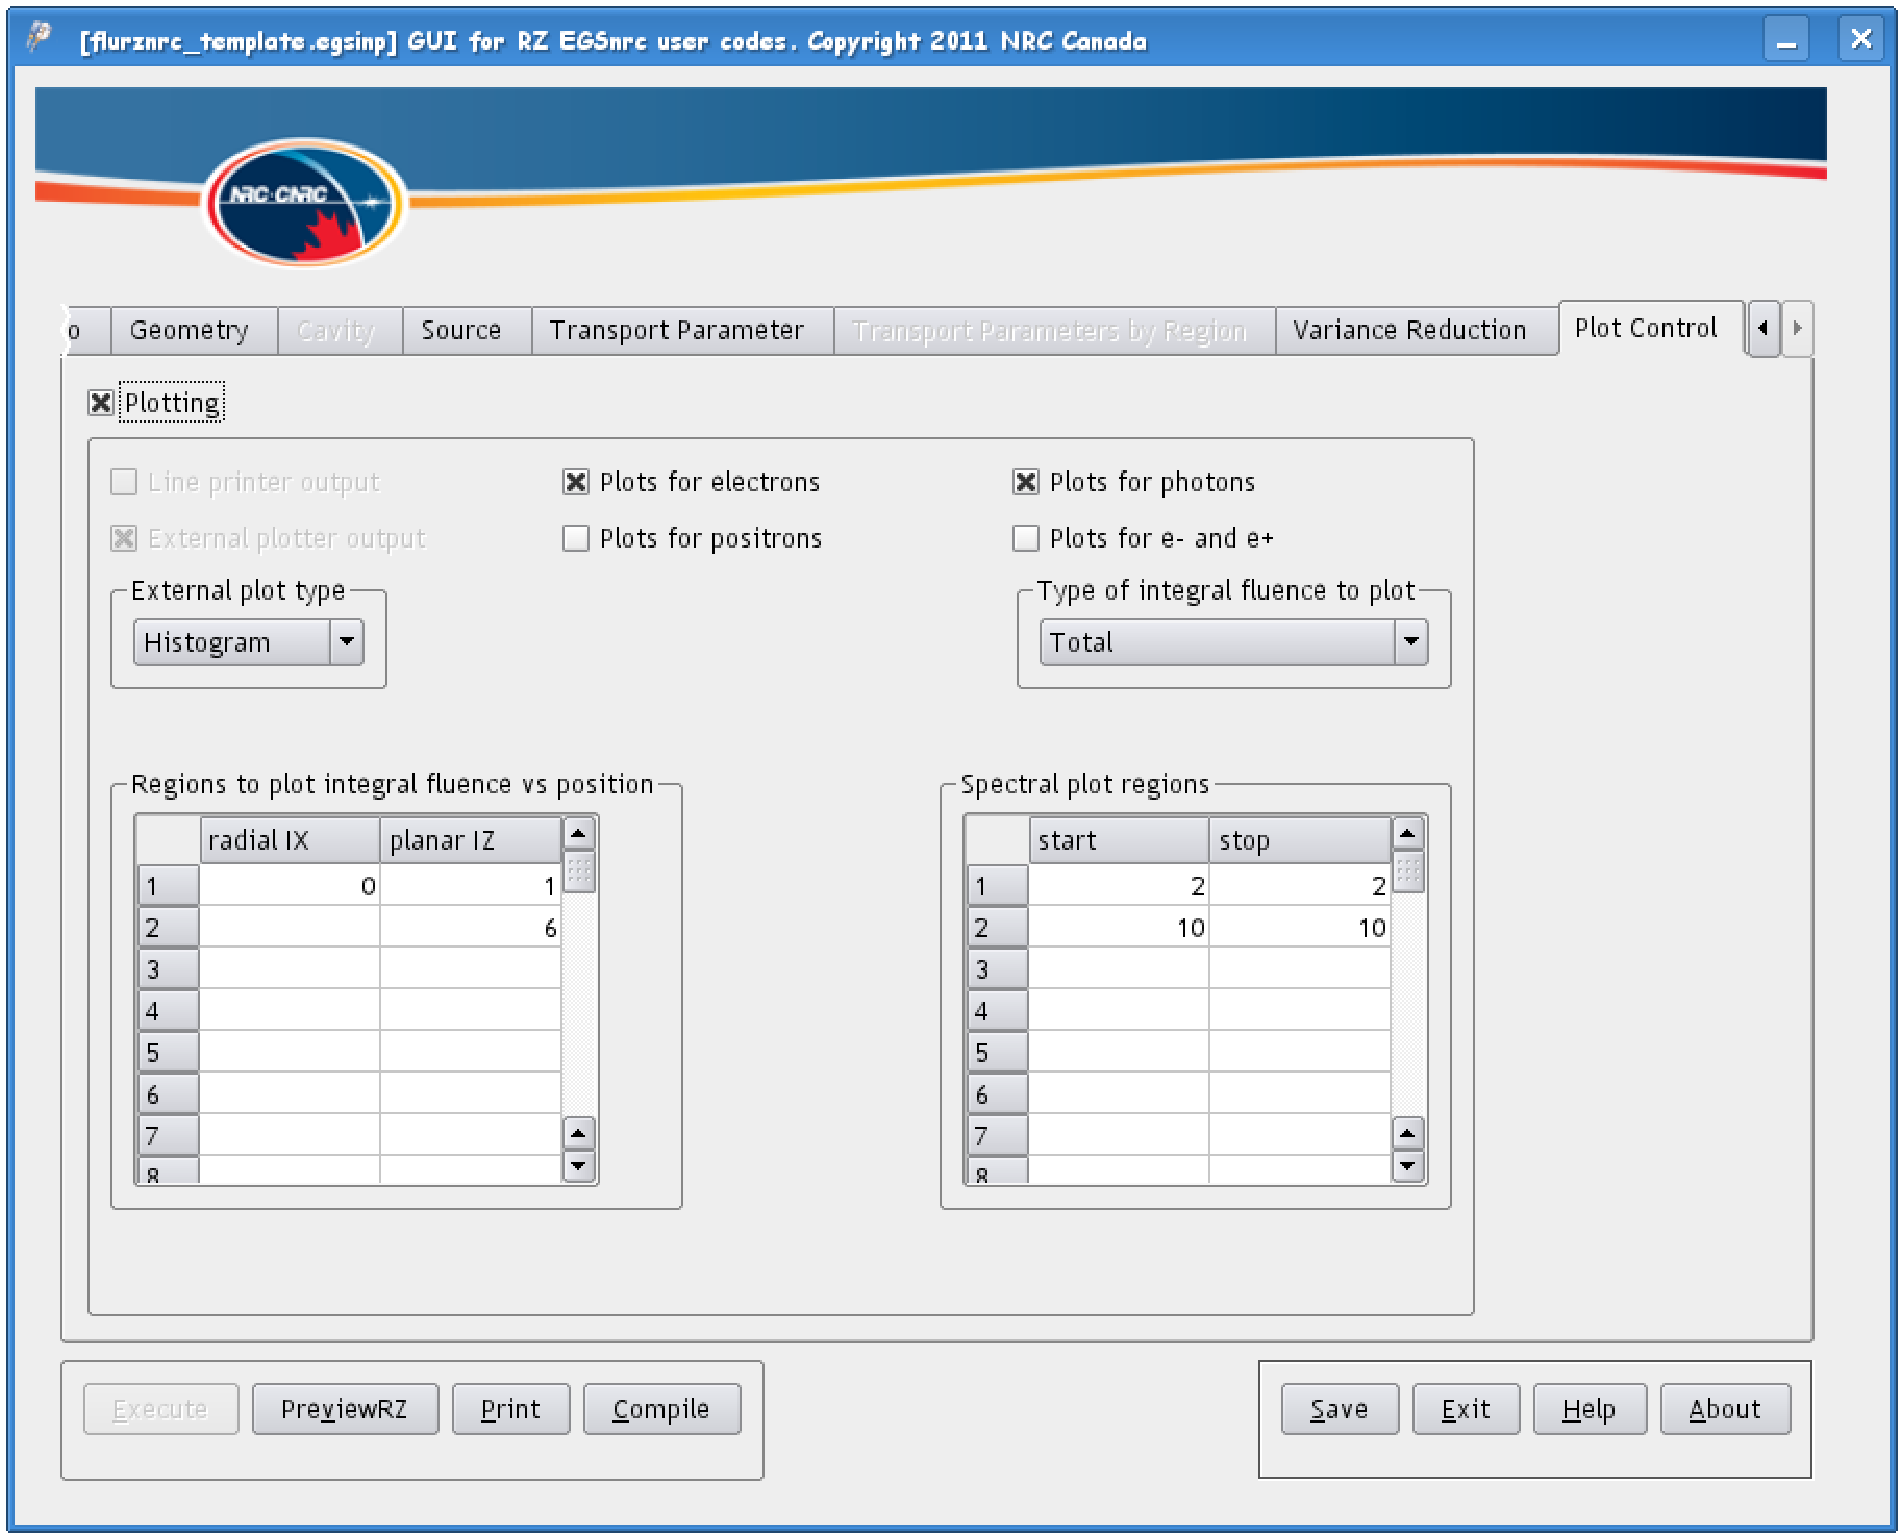
\includegraphics[height=11.56cm]{figures/plot_flurz}
\end{center}
\end{latexonly}
\begin{center}

\includegraphics[height=1mm]{figures/fake2}
\end{center}
\caption{Plot Inputs for the RZ EGSnrc User Code FLURZnrc.}
\label{plotflurz}
\end{figure}

% \newpage
\clearpage
% \renewcommand{\leftmark}{{REFERENCES}}
% \section{References}
\vspace*{-1.7cm}
\bibliography{../irs}
\typeout{}
\typeout{******REMEMBER to create .bbl  and reset twice**********}
\typeout{}
\bibliographystyle{unsrt}
\setlength{\parindent}{0em}
%\newpage
%\setlength{\baselineskip}{0.7cm}

% above defines style of .bbl file and must match the style of
%cite package used at start.
%other options are:
%\clearpage



\newpage
\typeout{**********starting index here******************}
\renewcommand{\leftmark}{{Index}}
%\renewcommand{\rightmark}{{Index}}
\addcontentsline{toc}{section}{\numberline{}Index}
\setlength{\baselineskip}{0.5cm}

%%%%%%%%%%%%%%%%%%%%%%%%%%%%%%%%%%%%%%%%%%%%%%%%%%%%%%%%%%%%%%%%%%%%%%%%%%%%%%%
%
%  EGSnrc egs_inprz manual
%  Copyright (C) 2015 National Research Council Canada
%
%  This file is part of EGSnrc.
%
%  EGSnrc is free software: you can redistribute it and/or modify it under
%  the terms of the GNU Affero General Public License as published by the
%  Free Software Foundation, either version 3 of the License, or (at your
%  option) any later version.
%
%  EGSnrc is distributed in the hope that it will be useful, but WITHOUT ANY
%  WARRANTY; without even the implied warranty of MERCHANTABILITY or FITNESS
%  FOR A PARTICULAR PURPOSE.  See the GNU Affero General Public License for
%  more details.
%
%  You should have received a copy of the GNU Affero General Public License
%  along with EGSnrc. If not, see <http://www.gnu.org/licenses/>.
%
%%%%%%%%%%%%%%%%%%%%%%%%%%%%%%%%%%%%%%%%%%%%%%%%%%%%%%%%%%%%%%%%%%%%%%%%%%%%%%%
%
%  Author:          Ernesto Mainegra-Hing, 2003
%
%  Contributors:    Iwan Kawrakow
%                   Frederic Tessier
%
%%%%%%%%%%%%%%%%%%%%%%%%%%%%%%%%%%%%%%%%%%%%%%%%%%%%%%%%%%%%%%%%%%%%%%%%%%%%%%%

%\documentclass[twoside]{article}	%has a hacked tocline def
%\documentclass[12pt]{article}		%use for drafting
\documentclass[12pt,twoside]{article}   %This screws up showkeys in references
\usepackage{graphicx}
%\usepackage{epsf}
%\usepackage{psfig}
%\usepackage{epsfig}
\usepackage{html}
\usepackage{amsmath} 
\usepackage{amssymb} 
\usepackage{fancyhdr}
%\usepackage{overcite}
\renewcommand{\footrulewidth}{0.4pt}
\renewcommand{\headrulewidth}{0.4pt}
%\usepackage{showkeys}			%use for drafting
%\newcommand{\captionl}[1]{\caption[#1]{#1}}   
%Does not work with showkeys but if use with listoftables and listoffigures 
%it generates a separate list of full captions as jornals require
%following works with showkeys on
\newcommand{\captionf}[1]{\caption[dummy]{\setlength{\baselineskip}{0.7cm} #1 \vspace*{2mm}\\}} 
\newcommand{\captionl}[1]{\caption[dummy]{ #1 \vspace*{2mm}\\}} 

% above for drafting with showkeys on
%
%\usepackage{overcite}
%following lines fix up style of bibliography to look just like
%in medical physics, i.e. superscripts

\setlength{\textwidth}{16.5cm}
\setlength{\headwidth}{16cm}		%for fancy page style only
\setlength{\textheight}{22.6cm} 
\setlength{\oddsidemargin}{-1mm}
\setlength{\evensidemargin}{-2mm} 
\setlength{\topmargin}{-1.5cm}
\setlength{\parindent}{1em} 
\setlength{\parskip}{1.3ex}
% \setlength{\floatsep}{0pt}
% \setlength{\textfloatsep}{0pt}		%space below a figure/table def 20pt
% \setlength{\intextsep}{0pt}		%space below a figure/table def 20pt
					%p142 compendium
\setlength{\abovecaptionskip}{5pt}

\newcommand{\eqn}[1]{\begin{equation} #1 \end{equation} }
\newcommand{\eq}[1]{Eq.(\ref{#1})}

%\newcommand{\Co}{$^{60}\mbox{Co}$}

\newcommand{\ie}{{\em i.e.}} 
\newcommand{\eg}{{\em e.g.~}}   
\newcommand{\etc}{{\it etc.}}
\newcommand{\vs}{{\it vs~}}
\newcommand{\viz}{{\em viz.~}}
\newcommand{\TM}{$^{\circledR}$}
\newcommand{\supcopyright}{$^{\copyright}$}       %

%Following is for Med Phys numbering  I.A.1  etc

%\renewcommand{\thesection}{\Roman{section}}
%\renewcommand{\thesubsection}{\thesection.\Alph.{subsection}}
%\renewcommand{\thesubsection}{\Alph{subsection}}
%\renewcommand{\thesubsubsection}{\arabic{subsubsection}}
%\renewcommand{\theparagraph}{\alph{paragraph}}
%\renewcommand{\thefootnote}{\fnsymbol{footnote}}


\newcommand{\cen}[1]{\begin{center} #1 \end{center}}

%\renewcommand{\contentsname}{}  %gets rid of word Contents at start of 
				%table of contents  p31 companion
\renewcommand{\refname}{}       %
%\newcommand{\chaptermark}[1]{\markboth{#1}{#1}} % remember chapter title
%\renewcommand{\sectionmark}[1]{\markright{\thesection\ #1}}
			 % section number and title

%[on even pages]{on odd pages}  %even only active twosided
				%if no even given, uses same for both
%lhead is left head, etc
\lhead[page~\thepage]{{\sf  egs\_inprz, a GUI for the NRC RZ user-codes}}
% \lfoot[{\sf \leftmark}]{{\small {\sf Last edited $Date: 2013/03/29 14:23:01 $
\lfoot[{\sf \leftmark}]{{\small {\sf Last edited: 2011/05/09 20:49:18
}}}
%\rhead[{\sf 1st author name }]{{\sf page~\thepage}}
\rhead[{\sffamily NRCC Report PIRS-801}]{{\sffamily ~\thepage}}
\rfoot[ ]{{\sf {\leftmark}}}
\cfoot{}
\chead{}


\typeout{***Have turned off overfull and underfull messages****}
\tolerance=10000        %suppress Overfull only
\hbadness=10000         %suppress Overfull and Underfull for text (horizontal)
\vbadness=10000         %suppress Overfull and Underfull for vertical "boxes"

\newcommand{\indexm}[1]{\marginpar{{\sf {\tiny I:#1} }}\index{#1}}
\makeindex

\begin{document}

%\DeclareGraphicsExtensions{.png}

\setlength{\baselineskip}{0.5cm}


\begin{htmlonly}

%Postscript versions of the entire paper are available.  You may have to
%download the compressed version to disk, uncompress or gunzip them and
%then read or print them.
%\htmladdnormallink{(uncompressed version 725 kb)}{ss96.ps}
%\htmladdnormallink{(compress version 233 kb)}{ss96.ps.Z}
%\htmladdnormallink{(gzip version 162 kb)}{ss96.ps.gz}


\begin{rawhtml}
Use the Up button to get back to this page from within the document.
<BR> <HR> <P>
\end{rawhtml}

\copyright
Copyright 2013, National Research Council of Canada
Ottawa

\begin{rawhtml}
<BR> <HR> <P>
\end{rawhtml}

\end{htmlonly}

\pagestyle{empty}

\title{User Manual for egs\_inprz}

\begin{center} 
{\sffamily \bfseries {\Huge User Manual for egs\_inprz, a GUI for the NRC RZ user-codes}
\vspace{5mm}\\}
\begin{Large}
Ernesto Mainegra-Hing \\
\end{Large}
Ionizing Radiation Standards\\
National Research Council of Canada
\\Ottawa, K1A OR6\\
\vspace{10mm}

\today \vspace{3mm}\\
\hfill NRCC Report {\sf PIRS-801}(RevB) \vspace*{10mm}\\

\begin{latexonly}
\begin{center}
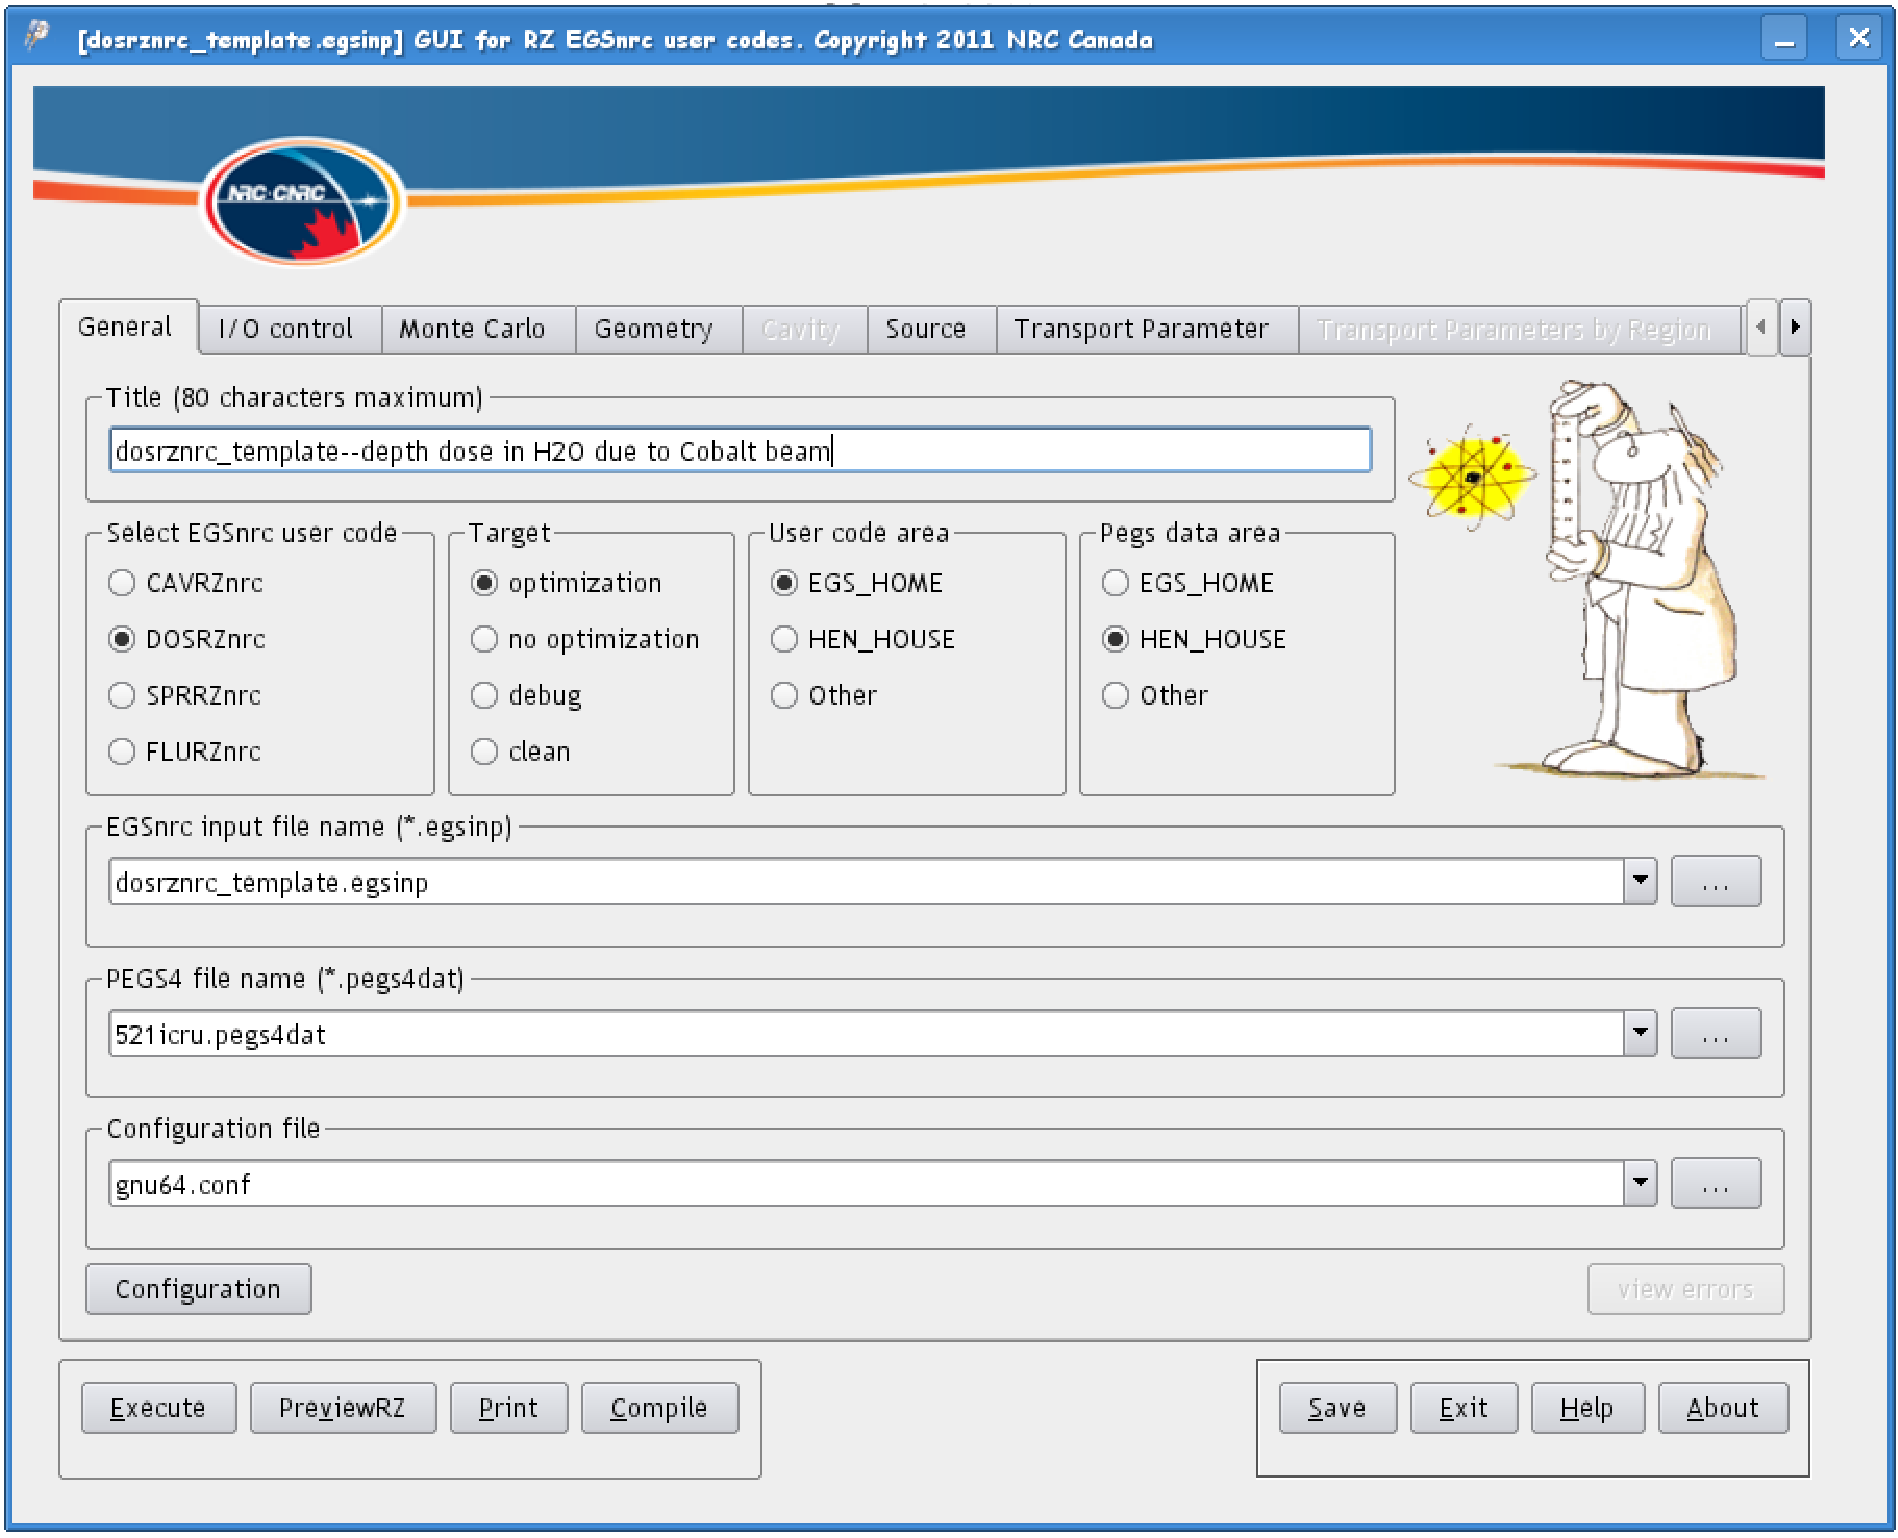
\includegraphics[height=11cm]{figures/main_page}
\vspace{5mm}
\\Front page of the egs\_inprz GUI for the RZ EGSnrc User Codes.
\vspace{10mm}\\
\end{center}
\end{latexonly}
\begin{htmlonly}
\begin{rawhtml}
<center>
<img src="figures/main_page.png">
<br><br>
Front page of the egs\_inprz GUI for the RZ EGSnrc User Codes. 
<br>
</center>
\end{rawhtml}
\end{htmlonly}

%\copyright NRC Canada, 2002 
\supcopyright NRC Canada, 2013

\end{center}
\newpage   %Blank page behind cover
\mbox{}

%\note{This page is intentionally blank to be the back of the front cover.
%Remove this note prior to printing!!!}


%\setcounter{page}{319}
\pagestyle{empty}

\pagestyle{fancy}



\newpage
\begin{abstract}

This is the reference user manual for {\bf \tt egs\_inprz}, a graphical user interface
for the EGSnrc RZ user-codes suite. It briefly introduces the GUI and describes how 
to install it and work with it. Descriptions and snapshots of each of the input blocks 
are provided.

\end{abstract}



\noindent
This code is distributed under the GNU Affero General Public License 3.0.


\tableofcontents


\newpage

\section{Introduction}

One of the major improvements in the RZ user-codes was moving from an input format
based on a long series of numbers to a text based input which is easier to use.
This text based system for input files was then used to create a single routine 
({\tt get\_inputs}) to read inputs entries for all the user codes so that now 
one can cut and paste entire input blocks from one user code to another. 
This routine is now part of the EGSnrc system and can be used in any user-code to 
parse through {\tt key=value} pairs in an input file.
As a consecuence, input files look very similar and,
more importantly, they are much easier to read and know exactly what the simulation 
is about without having the description of the inputs open on the desk. 
The idea behind using a GUI for working with EGSnrc input files is to further 
extend the above mentioned improvements. Although the input files are currently 
very readable, one must still remember what the keys used in an input file mean.
By using this GUI, a user can immediately get a description about any input parameter
by means of tool-tips.

{\tt egs\_inprz} is a Graphical User Interface (GUI), originally created for manipulating
(reading, creating, modifying, printing and visualizing) 
input files for the  RZ suite of EGSnrc  user-codes:
DOSRZnrc, CAVRZnrc, SPRRZnrc and FLURZnrc (see NRCC report PIRS-702\cite{Ro10}). 
Furthermore it can be also used for compiling and executing these user-codes. 
% There is also an option for creating new configurations (combinations of compiler settings 
% with platform specific libraries).
% \index{config files}
\index{RZ user-codes}
 {\tt egs\_inprz} is user friendly, offering more flexibility, on-line help and therefore, 
increases the efficiency in getting hands-on experience with the EGSnrc user codes.

 This GUI was developed using Qt, a multi-platform, C++ Graphical User Interfaces toolkit
 that enables building efficient, portable and maintainable GUI applications 
 quickly and easily. Qt is a fully object-oriented, easily extensible C++ application  
 framework that enables rapid building of state-of-the-art GUI applications. For more
 information please see \htmladdnormallink{{\sf 
 http://www.qt.io/.}}
{http://http://www.qt.io/}
\index{Trolltech}
\index{Qt library}


\newpage
\section{Installation}
\label{installation}

\index{installation}

\index{EGSnrcMP}
This GUI is part of the multi-platform version\cite{Ka03} 
of the EGSnrc Monte Carlo simulation system\cite{Ka09a}.
For its development we used the Qt library and therefore,
users wanting to build it, will have to install this library. Most Linux distributions include the
Qt library these days, since the popular Desktop Environment KDE is based on this library. However,
if the Qt library is not available in the user's system, one needs to install it first

Only Linux/Unix users need to built this GUI since it is distributed as a binary executable on
Windows. We might start distributing binary executables for Linux/Unix as well in the near future.
The only requirement for this to happen is that most Linux distributions and Unixes are binary
compatible and the GUI is linked statically to the Qt library.

\index{KDE}
\index{Qt INSTALL file}



\subsection{Building {\tt egs\_inprz}}
\label{building}
\index{QTDIR}      
\index{building egs\_inprz}

\index{compiling {\tt egs\_inprz}}
The user can have this and the other GUI's built during installation of the EGSnrc system,
provided {\tt QTDIR} is properly set. At any time the user can go to 
{\tt \$HEN\_HOUSE/gui/egs\_inprz} and type

      {\tt ./make [EGS\_CONFIG=desired\_config]}

\noindent A C++ compiler will have to be installed on
your computer in order to build the GUIs. 
On Windows one {\bf must} have installed either MS C++ 6.0 or Borland C++.

\noindent {\bf Note:} You only need to pass {\tt EGS\_CONFIG} to {\tt make} if it is not set
or you want/need to build the GUI for a different configuration as the current one. 
In principle, all Makefiles provided in the new EGSnrcMP environment are for {\tt GNU make}.
Although they might also work with other Unix {\tt make} versions.

It is important that the environment variable {\tt QTDIR} points to the location where 
Qt was installed. This can be checked by issuing the command:

      {\tt echo \$QTDIR} on Unix/Linux or

      {\tt echo \%QTDIR\%} on a Windows console.
      
One can change this environment variable by issuing the command

      {\tt setenv QTDIR Qt\_location} for the C shell, or

      {\tt export QTDIR = Qt\_location} for Bash, or

      {\tt set QTDIR=Qt\_location} on a Windows console.

{\bf On Unix/Linux} this variable can be set on a system wide basis by including the 
corresponding statement above in the {\tt .cshrc} resource file for the C-shell or 
the {\tt .basrc} resource file for Bash.

{\bf On Windows} the user can also set the QTDIR environment variable system wide by
right clicking on the {\tt My Computer} icon, selecting {\tt Properties} and clicking on the
{\tt Environment Variables} button in the {\tt Advanced} tab.
  
\newpage
\section{Using {\tt egs\_inprz}}
\subsection{Running {\tt egs\_inprz}}
\index{executing}
\index{HEN\_HOUSE}

After installing EGSnrc, {\tt egs\_inprz} is located on {\tt HEN\_HOUSE/bin/my\_machine/}.
{\tt my\_machine} stands for the name of the configuration used to build the GUI. For more
information about configurations the user is referred to the PIRS-877 report on the new
multi-platform environment\cite{Ka03}.

{\bf On Windows} the user can invoke directly the binary executable from a DOS console, since its 
location will be on the user's PATH environment variable. If requested by the user, there will
be also shortcuts to the GUI's distributed with the EGSnrc system on the Desktop and 
Start Menu.
\index{executing!Windows}

{\bf On Unix/Linux} the user can also invoke directly the binary executable from a shell console, 
since its location is added to the user's PATH environment variable when the corresponding
{\tt egsnrc\_[cshrc|bashrc]\_additions} is sourced, which {\bf must} have been done after 
installing the EGSnrc system.
The alias {\tt egsinprz} is 
also available, which points to {\tt HEN\_HOUSE/bin/my\_machine/egs\_inprz} and starts the GUI 
in the background.
If requested by the user, shortcuts for the KDE desktop environment are also created by the 
installation GUI.
\index{executing!Unix/Linux}

Once all the necessary information is entered, the user can perform different operations 
from within the GUI provided the input file has been saved to the disk since all other 
operations use the disk version of the input file.


\subsection{Reading EGSnrc RZ input files}
\label{reading}
\index{input files!reading}

Existing input files can be read directly from the command line by passing the file name as 
argument, i.e., by invoking

        {\tt egs\_inprz} {\em filename[.egsinp]}

\noindent
where the file name can be with or without extension. If the file does not exist, a warning
message is shown and the file name {\tt new\_file.egsinp} is used instead. Note, that in this
case no input file will exist. To have an actual input file and be able to run a calculation, 
the user {\bf must} have saved it. Saving {\tt new\_file.egsinp} without modifying any entry
will leave a default input file for use with the RZ user code {\tt dosrznrc.mortran}.

Once an existing input file is loaded, it is  
searched to identify the user-code it belongs to. If no user-code is identified, 
DOSRZnrc is used by default. Once the user-code to be used is known, its location
becomes the place where the GUI will look for input files.

Regarding location, the EGSnrc system relies on having the input file on the EGSnrc
user area, \ie, {\tt EGS\_HOME/user-code}. This is so because for execution,
temporary directories and output files are created, moved and deleted and all these 
operations are relative to the {\tt EGS\_HOME/user-code} location.

For this reason, this GUI will only store input files in the user's EGSnrc
area, i.e., {\tt EGS\_HOME/user-code}. If the EGSnrc user area does not exist, 
the GUI creates it and issues a warning.
\index{input files!location}
\index{EGS\_HOME}

Input files can be also read in from the GUI's General tab. Once the GUI is loaded, 
a list of available {\em *.egsinp} input files in the current directory is offered 
to the user through the EGSnrc input file name combo box. By default the input file 
template {\em dosrznrc\_template.egsinp}, distributed with the EGSnrc system, is loaded.
Alternatively, the user can click on the button to the right of the combo box to 
invoke an open file dialog to open any {\em *.egsinp} file located anywhere.
\index{.egsinp}

The GUI verifies that all media used in the input file are available in the selected
PEGS4 data set. By default this file is set to be {\tt 521icru.pegs4dat}, a standard data 
file, that comes with the EGSnrc distribution. If any medium is not found in the 
current PEGS4 data file, an error message pops up recommending that the user corrects the
media names and/or find the appropriate data file.
\index{PEGS4}
\index{pegs4 media}

\index{user-code area}
The user-code area is the location where {\tt egs\_inprz} will look for input files. Initially, 
{\tt egs\_inprz} assumes that the user-code area is {\tt EGS\_HOME/user-code}, where {\tt user-code} 
is by default {\em dosrznrc}. If the GUI is started from any user-code location, {\tt user-code} 
is changed to the corresponding user-code. If a valid input file name is passed as argument to 
{\tt egs\_inprz}, then after identifying the user-code, {\tt user-code} is updated properly. 
The user-code area can 
be later changed by the user in the general input tab (see figure \ref{generalfig} in section 
\ref{general}).

\index{PEGS4-data area}
Similarly, the PEGS4 data area is the location where {\tt egs\_inprz} will look for PEGS4 data sets. 
Since
there are some data sets in the EGSnrc distribution, we chose to set this area to be in 
{\tt HEN\_HOUSE/pegs4/data} by default. Later on, when users have created their own data sets, they 
can switch to {\tt EGS\_HOME/pegs4/data} or any other location of their preference.


\subsection{Creating EGSnrc RZ input files}
\label{creating }
\index{input files!creating}

As mentioned above, when starting the RZ GUI, the template {\tt dosrznrc\_template.egsinp} is 
read in, which contains defaults for all possible entries. Saving this template under any other 
name is a possible way for getting started. In similar fashion, one can switch to another RZ 
user-code (see section \ref{general}) and select the corresponding input template file.
\index{default input file}

\subsection{Porting input files between NRC RZ user-codes}
\label{modifying}
\index{input files!porting}

 Sometimes different user-codes share common input blocks like transport parameters,
 geometry, variance reduction parameters, and so on. For instance,
 the user might want to run a CAVRZnrc calculation to obtain the dose inside the air
 cavity of an ion chamber and also run a FLURZnrc calculation to obtain the spectrum
 inside the cavity for the same chamber. This is easily acomplished with {\tt egs\_inprz}
 by loading the input file for the CAVRZnrc calculation, switching to the other user 
 code input by  clicking on the corresponding radio button in 
 the user-code group box (see figure \ref{generalfig} in section \ref{general}). 
One will have to modify the default entries for the selected user-code to suit the user's
problem if needed. Once the proper entries are made, the input file can be saved by 
clicking on the {\em Save} or {\em Save\&Exit} button  
in the user's EGSnrc user-code area (if it doesn't exist, it is created automatically, 
 and a warning is issued to the user).\\

\subsection{Viewing the geometry with previewRZ}
\index{previewRZ}
\index{geometry!visualizing}
\index{input files!previewRZ}

Once an existing input file has been loaded or created from scratch and saved on 
the hard drive,
the user can invoke 
{\tt previewRZ}, a tool supplied with the EGSnrc distribution, which allows one 
to visualize the geometry and material data (see figure \ref{view}). 
The {\tt PreviewRZ} button, placed in the left bottom corner of the GUI
(see any GUI snapshot in section \ref{screenshots}), 
becomes enabled if Tcl/Tk is installed on your computer, the input file exists 
and there were no errors reading the geometry. Pressing this button is equivalent 
to typing on the command line of a console (Windows or Unix/Linux)

 {\tt HEN\_HOUSE/previewRZ/previewRZ name[.egsinp]}
 
\noindent where the input filename can be entered with or without extension. \\

\begin{figure}[h]
\begin{htmlonly}
\begin{rawhtml}
<p><center>
<img width=486 height=629 src="figures/previewrz.png"><br><br>
</center>
\end{rawhtml}
\end{htmlonly}
\begin{latexonly}
\begin{center}
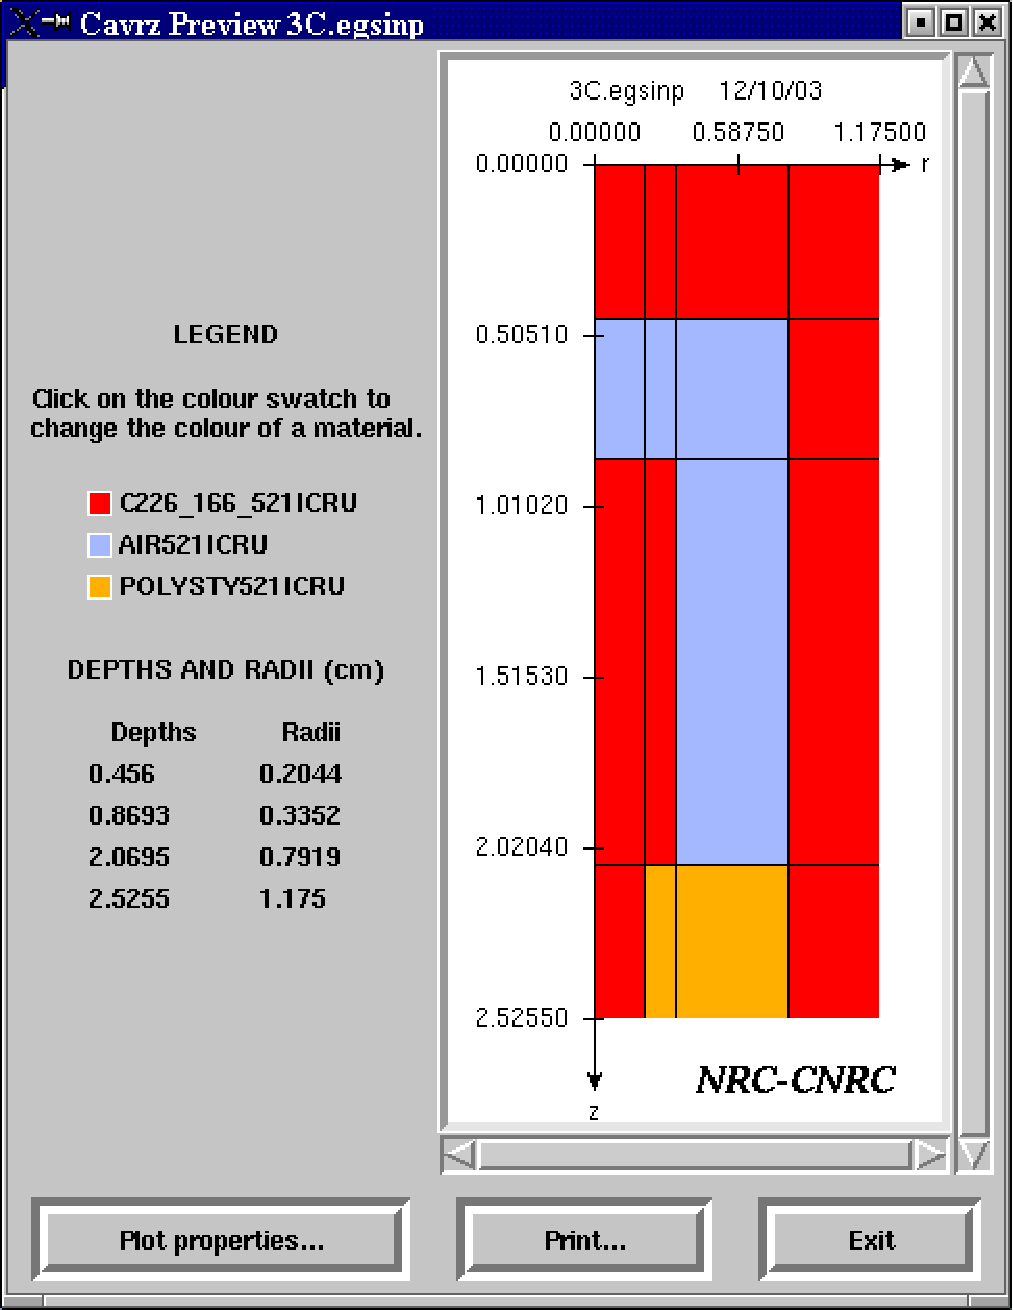
\includegraphics[height=9cm]{figures/previewrz}
\end{center}
\end{latexonly}
\begin{center}

\includegraphics[height=1mm]{figures/fake2}
\end{center}
\caption{View of a 3C cylindrical ionization chamber using {\tt previewRZ}.}
\label{view}
\end{figure}

{\tt previewRZ} is a Tcl/Tk script 
which had been previously used at NRC only on Unix/Linux. We have now successfully used 
{\tt previewRZ} on Windows 2000/XP after downloading and installing a Tcl/Tk 
self-extracting distribution. 
To find out whether
Tcl/Tk is available on the user's system, {\tt egs\_inprz} tries to find the binary 
executable {\tt wish.exe} on Windows or {\tt wish} on Unix/Linux in any of the locations 
defined on the user's PATH environment
variable.
The Tcl/Tk package is {\bf FREELY} distributed for HP-UX, Linux, 
Solaris, and Windows by ActiveState Corp. 
To obtain  Tcl/Tk go to
\htmladdnormallink{{\sf 
 http://www.activestate.com/Products/ActiveTcl/}}
{http://www.activestate.com/Products/ActiveTcl/}
and click on the {\tt Download} link of the page. For more information and useful links
on Tcl/Tk please visit
\htmladdnormallink{{\sf 
http://www.tcl.tk/software/tcltk/}}
{http://www.tcl.tk/software/tcltk/}
\index{Tcl/Tk}
\index{Active State Corp.}
\index{wish}

Future versions of the {\tt egs\_inprz} GUI will use its own
previewing tool, but for now, users wishing to have the feature of looking
at the geometry they are defining, will have to install the Tcl/Tk package.

\subsection{Printing *.egsinp input files}
\index{input files!printing}

 To produce a hard copy of the input file, users have the option to print the file
 by pressing the {\tt Print} button located in the button group on the lower left 
 corner of the GUI (see any GUI snapshot in section \ref{screenshots}). A Print 
 Dialog pops up with a list of available printers and a printer and  paper format 
 setup among other options (see figure \ref{print}).\\
 
\begin{figure}[htb]
\begin{htmlonly}
\begin{rawhtml}
<p><center>
<img width=517 height=606 src="figures/printer_dialog.png" name=print><br><br>
</center>
\end{rawhtml}
\end{htmlonly}
\begin{latexonly}
\begin{center}
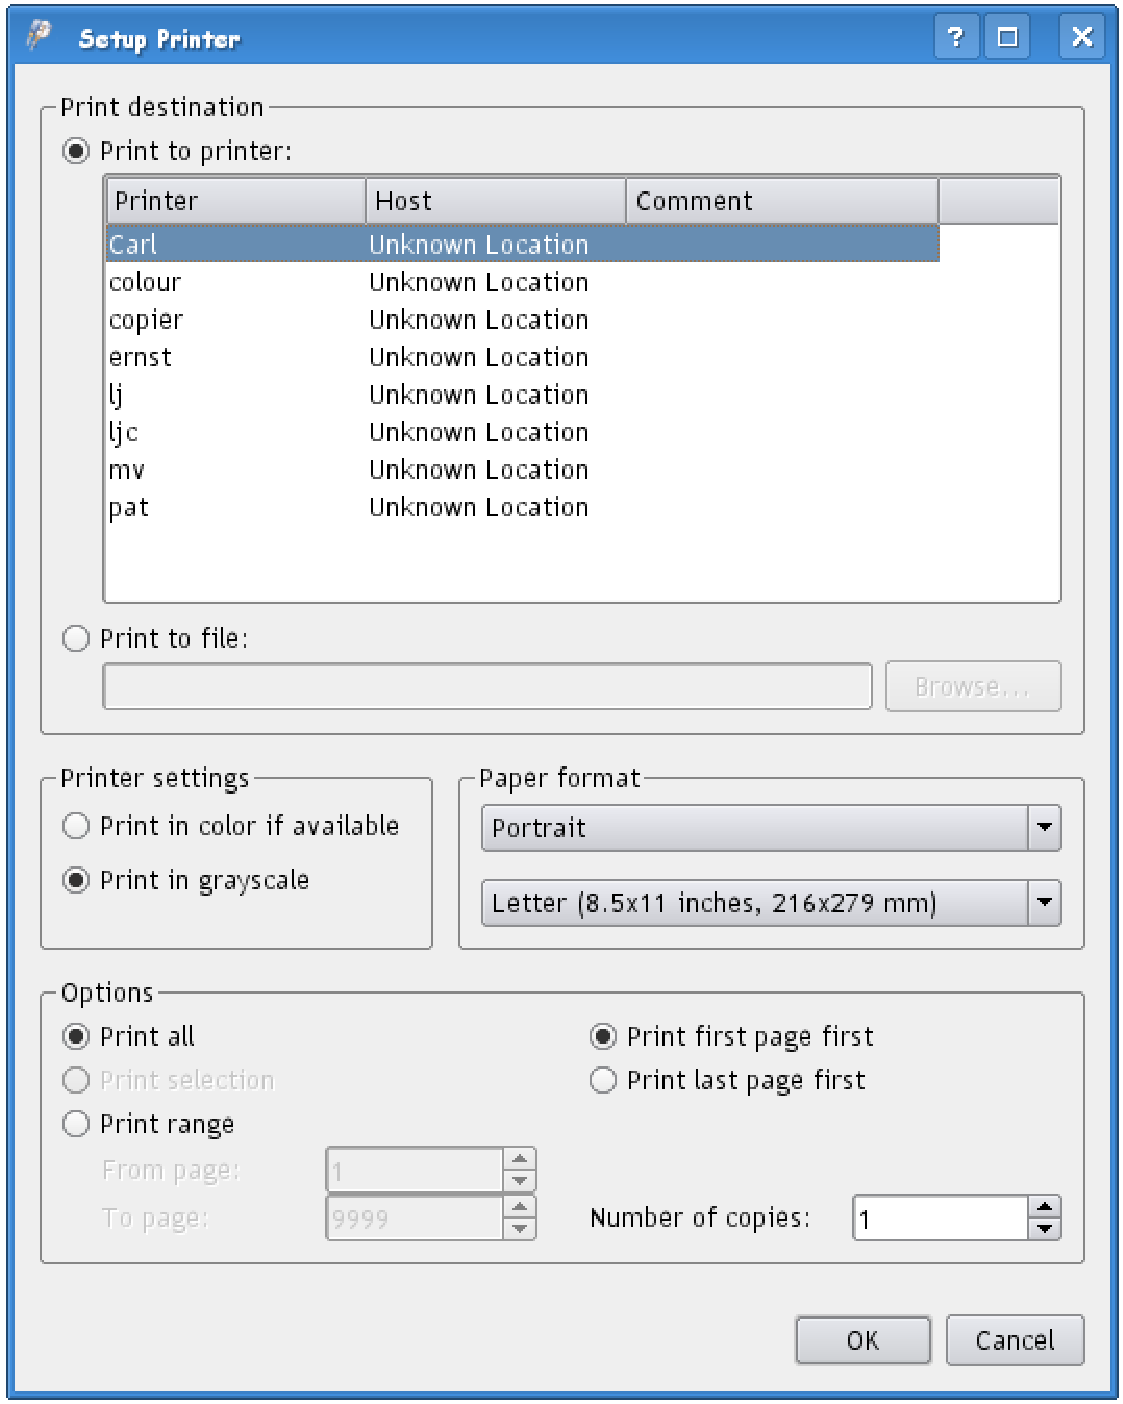
\includegraphics[height=9cm]{figures/printer_dialog}
\end{center}
\end{latexonly}
\begin{center}

\includegraphics[height=1mm]{figures/fake2}
\end{center}
\caption{\label{print}Printer Setup Dialog on SuSE Linux 10.3 KDE 3.5.9}
\end{figure}

\subsection{Compiling the RZ user codes}
 
When one modifies the user-codes, these need to be re-compiled. 
The user can perform
this operation from within the GUI by pressing the {\em Compile} button on the  lower left 
corner of the GUI (see for instance figure \ref{generalfig} in section \ref{general}). 
On the {\tt General Information} tab there is a {\tt Target} radio button group box where
one can choose the type of compilation desired. By default it is set to {\tt optimization}
which uses the optimization option defined in the active config file generated during the 
EGSnrc installation process or the configuration utility available in all the EGSnrcMP GUI's.
The other available options are {\tt no optimization, debug and clean}.
Optimization is recommended for production runs after the user-code
and the input file have been thoroughly tested.

\subsection{Executing the RZ user codes}

After all necessary information has been entered and stored, one can execute the EGSnrc 
RZ user-code from within the GUI by pressing the {\em Execute} button on the  lower left 
corner of the GUI (see figure \ref{generalfig} in section \ref{general}). A dialog appears 
where one can define the different execution parameters (see figure \ref{execution}). 
There are two modes for running an EGSnrc RZ user-code, {\it interactive} or {\it batch}, \ie, 
using a batch queuing system. The execution mode defaults to {\it interactive}. 
The {\it batch} execution mode is only available on Unix/Linux since it has not 
been implemented on Windows yet.
At NRC the {\em PBS batch system} is currently used to send jobs to a queue where 
they are remotely executed, returning the results after completion to the 
user EGSnrc area.
 
% \begin{figure}[tbp]
\begin{figure}[h]
\begin{htmlonly}
\begin{rawhtml}
<p><center>
<img src="figures/execution.png" name=execution><br><br>
</center>
\end{rawhtml}
\end{htmlonly}
\begin{latexonly}
\begin{center}
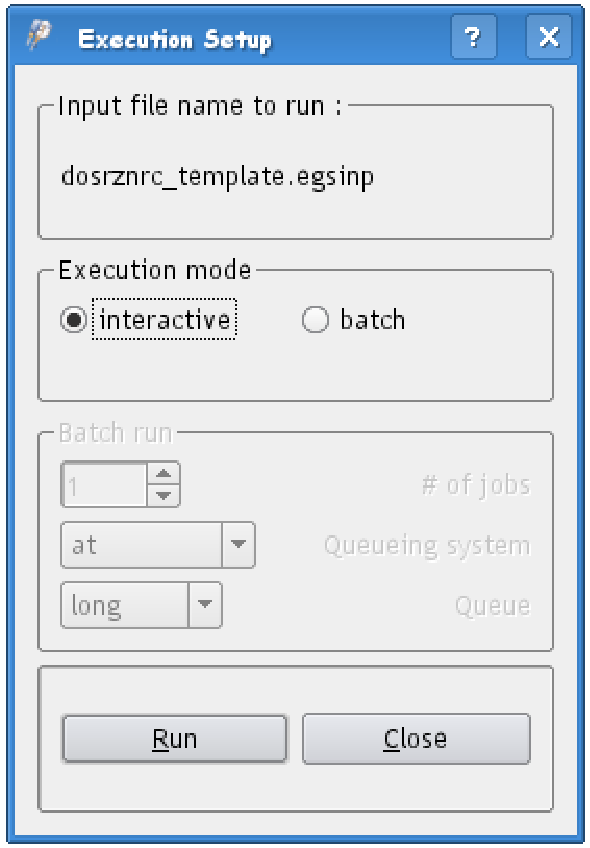
\includegraphics[height=11cm]{figures/execution}
\end{center}
\end{latexonly}
\begin{center}

\includegraphics[height=1mm]{figures/fake2}
\end{center}
\caption{Execution Setup Dialog.}
\label{execution}
\end{figure}

{\bf On Unix/Linux} if the batch execution mode is selected, a pane becomes enabled where
queue input parameters can be entered such as the queueing system, type of queue 
and number of jobs to submit (see figure \ref{batchexecution}). 
The GUI recognizes which queueing systems are available 
by looking up on {\tt \$HEN\_HOUSE/scripts} for batch definition files in the form 
{\tt batch\_options.queueing\_system},
where {\tt queueing\_system} stands for either {\tt at}, {\tt nqs} or {\tt pbs}. The user
can add any other batch submission system by creating a batch definition file in a similar 
fashion to the ones in the EGSnrcMP distribution.

The default batch submission system assumed in the GUI is the standard Unix
job submission tool {\tt at}. The batch definition files provided in the directory 
{\tt \$HEN\_HOUSE/scripts} contain specific definitions for the {\tt at}, 
{\tt NQS} and {\tt PBS} batch submission systems. If the user wants to make NQS, PBS or 
any other system the default job submission system,
he/she can define the environment variable {\tt EGS\_BATCH\_SYSTEM} to be nqs, pbs or
the name of the other queueing system.
\index{EGS\_BATCH\_SYSTEM}
\index{queueing system}
\index{batch runs}
\index{batch\_options}

These are the batch definition files distributed with the EGSnrc system:
\begin{description}
\item {\tt batch\_options.at}
\item {\tt batch\_options.nqs}
\item {\tt batch\_options.pbs}
\end{description}
\index{batch\_options}
\index{queueing system}

Queue names are installation especific and at NRC the 
names {\em short}, {\em medium} and {\em long} have been adopted for {\tt PBS} and {\tt NQS}. 
To change these, edit the names
in the proper batch definition file.

For more information on the implementation of parallel runs in the new EGSnrc system, the reader
is refered to the NRCC report PIRS-877.

\begin{figure}[h]
\begin{htmlonly}
\begin{rawhtml}
<p><center>
<img src="figures/execution_batch.png" name=batchexecution><br><br>
</center>
\end{rawhtml}
\end{htmlonly}
\begin{latexonly}
\begin{center}
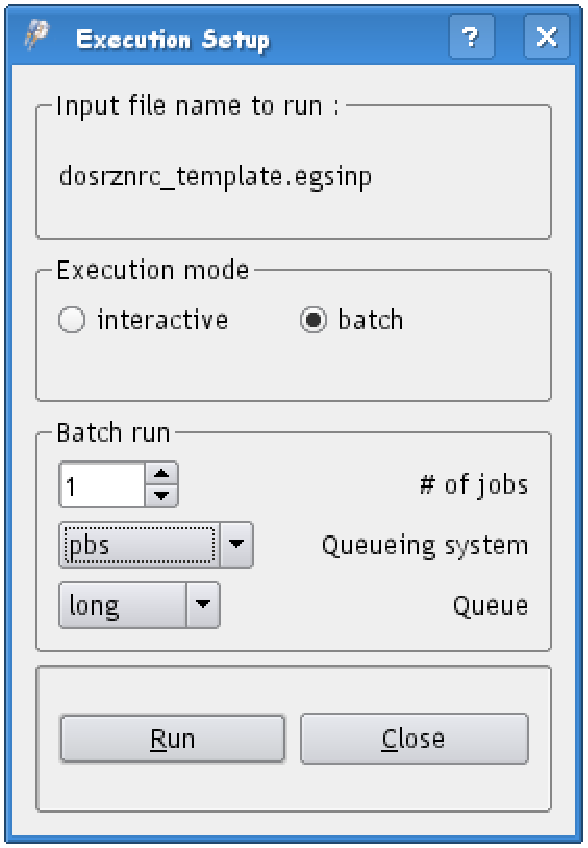
\includegraphics[height=11cm]{figures/execution_batch}
\end{center}
\end{latexonly}
\begin{center}

\includegraphics[height=1mm]{figures/fake2}
\end{center}
\caption{Execution Setup Dialog in batch mode.}
\label{batchexecution}
\end{figure}

\clearpage

% 
% \section{Creating and modifying config files}
% 
% A key element in the new EGSnrcMP multi-platform environment is the config file,
% which contains important system definitions allowing the use of EGSnrc on different
% Operating Systems and with different compilers. A detailed description of config
% files and definition of what constitutes a configuration can be found in the technical
% report PIRS-877\cite{Ka03}.
% 
% \begin{figure}[htb]
% \begin{htmlonly}
% \begin{rawhtml}
% <p><center>
% <img src="figures/configure.png" name=config><br><br>
% </center>
% \end{rawhtml}
% \end{htmlonly}
% \begin{latexonly}
% \begin{center}
% 
\includegraphics[height=10cm]{figures/configure.png}
% \end{center}
% \end{latexonly}
% \begin{center}
% 
\includegraphics[height=1mm]{figures/fake2}
% \end{center}
% \caption{Configuration Wizard.}
% \label{config}
% \end{figure}
% 
% From within {\tt egs\_inprz}, users can modify existing config files and
% create new ones by clicking on the {\tt Configuration} button found on the General 
% Information tab. A reduced version of the {\tt egs\_install} Wizard appears where
% one can define the Fortran and C compilers and set the names for the config file and 
% the configuration (figure \ref{config}). Once all the required information has been 
% entered, the Wizard 
% runs a series of tests for the selected Fortran and C compilers on the running 
% operating system. The
% results of these tests are used to create the system/compiler dependent
% files {\tt machine.mortran} and {\tt machine.macros}.  The configuration
% utility then starts the actual building of the EGSnrc system, by
% creating the Mortran3 string processor {\tt mortran3.exe} and the PEGS4
% data pre-processing tool {\tt pegs4.exe}.

\section{Getting help}
\label{help}

One of the advantages of a graphical user interface is the possibility of providing 
information in an interactive way. {\tt egs\_inprz} uses this feature extensively by 
activating so called {\em tool tips} when the user positions the mouse over a given area
in the GUI. A dialog pops up {\em temporarily} with information, if available, about the 
corresponding input quantity. 

There is also the possibility of activating these {\em tool tips} {\em permanently} (until 
another action is performed: mouse click or key press). For this, the user must set the focus 
on the relevant location and press {\tt Shift+F1}. The help text appears immediately; it goes 
away as soon as the user does something else.

More general information is provided in html format through the {\em Help} button located 
in the lower right corner of the GUI ({\em html} version of this document).
{\tt egs\_inprz} attemps to run {\em Internet Explorer} on Windows and
{\em Konqueror} or {\em Netscape} on Unix/Linux to show the document. If none of these 
are available an error message is displayed. In that case the user can go to {\tt \$HEN\_HOUSE/gui/egs\_inprz/html} and load the index page {\em index.html} with an html 
browser of his/her choice.

\section{Input blocks description and screenshots}
\label{screenshots}

In this section we describe briefly the different input blocks that are used in the NRC 
RZ user codes.
We have also included screenshots of the different input tabs of the GUI. In each 
of these tabs, there are input options, common to all the RZ user codes. But some of them are
specific to one user code and remain disabled when one selects a different user code.
The active file name is always displayed on the GUI's caption. This can be useful to recognize
whether the current file name in the input box is the same as the active one.

{\bf Note} that the bottom row of buttons are available with all tabs.


\newpage
\subsection{The General Information Tab}
\label{general}

As its name suggests, this section of the tabbed dialog is intended to collect general 
information not contemplated inside the input file itself like the input and pegs4 data 
file names, the areas to search for those files, compilation mode, execution mode and 
its parameters, 
the user code name, etc. The title constitutes an exception, since it is part of the input 
file, but does not fit in any of the different input blocks.

A very useful feature in this GUI is the ability to set the location of the input and 
pegs4 files automatically to be in the {\tt HEN\_HOUSE} or {\tt EGS\_HOME} area. This saves
time by not having to browse all the way to the location of different files, acting like 
a shortcut. If the files are loaded from a location different than the above
mentioned, the {\tt Other} radio button is checked. Note that upon loading an input file
from a location other than the {\tt HEN\_HOUSE} or {\tt EGS\_HOME} user code area, it will
be only saved on the {\tt EGS\_HOME} user code area. \\ \\
\begin{figure}[htb]
\begin{htmlonly}
\begin{rawhtml}
<p><center>
<img src="figures/general.png" name=generalfig><br><br>
</center>
\end{rawhtml}
\end{htmlonly}
\begin{latexonly}
\begin{center}
\includegraphics[height=10.78cm]{figures/general}
\end{center}
\end{latexonly}
\begin{center}
\includegraphics[height=1mm]{figures/fake2}
\end{center}
\caption{General Input for the RZ EGSnrc User Codes.}
\label{generalfig}
\end{figure}

\newpage
\subsection{The I/O Control Tab}
\label{io}

This block contains information relevant to the I/O controls of the NRC user codes. 
Many of the inputs are common to all codes, but there are some which are specific to 
only some of them. \\ \\
\begin{figure}[htb]
\begin{htmlonly}
\begin{rawhtml}
<p><center>
<img src="figures/io.png" name=io_control><br><br>
</center>
\end{rawhtml}
\end{htmlonly}
\begin{latexonly}
\begin{center}
\includegraphics[height=10.78cm]{figures/io}
\end{center}
\end{latexonly}
\begin{center}
\includegraphics[height=1mm]{figures/fake2}
\end{center}
\caption{I/O control for the RZ EGSnrc User Codes.}
\label{io_control}
\end{figure}


\newpage
\subsection{The Monte Carlo Parameter Tab}
\label{mc}


This input tab collects the typical information required in a Monte Carlo simulation like
the number of histories to run, the initial random number seeds, desired statistical accuracy,
and the maximum CPU time for the calculation. There are also more user code specific entries
that are enabled or disabled depending on the user code selected.

An input block required only by the user code DOSRZnrc when the calculation type is 
{\em pulse height distribution} is also included in this tab. For other calculation types and user codes,
this box remains disabled. \\ \\

% The command below does not work !!!
%\DeclareGraphicsRule{.tiff}{eps}{.tiff.bb}{'convert #1 'eps:-'}

\begin{figure}[htb]
\begin{htmlonly}
\begin{rawhtml}
<p><center>
<img src="figures/mc.png" name=mc_control><br><br>
</center>
\end{rawhtml}
\end{htmlonly}
\begin{latexonly}
\begin{center}
\includegraphics[height=11.56cm]{figures/mc}
\end{center}
\end{latexonly}
\begin{center}
\includegraphics[height=1mm]{figures/fake2}
\end{center}
\caption{Monte Carlo parameters for the RZ EGSnrc User Codes.}
\label{mc_control}
\end{figure}


\newpage
\subsection{The Geometry Tab}

This input block contains all the necessary inputs for defining a RZ geometry (cylindrical symmetry) 
and the media present in the different regions. It is important to notice that for the user code 
CAVRZnrc an option is available to define the geometry in a simpler way. If the input method selected
(upper left corner of the tab) is {\em cavity description}, then the rest of the input fields in this 
tab are disabled and the whole geometry input occurs through the next tab, {\tt the cavity tab}.

Only media present in the current PEGS4 data set can be set in the media table. This is assured by
activating a combo box in the first column of the media table as soon as the user tries to type
or double click on it. \\ \\

\begin{figure}[htb]
\begin{htmlonly}
\begin{rawhtml}
<p><center>
<img src="figures/geometry.png" name=geometry_control><br><br>
</center>
\end{rawhtml}
\end{htmlonly}
\begin{latexonly}
\begin{center}
\includegraphics[height=11.56cm]{figures/geometry}
\end{center}
\end{latexonly}
\begin{center}
\includegraphics[height=1mm]{figures/fake2}
\end{center}
\caption{Geometry Input for the RZ EGSnrc User Codes.}
\label{geometry_control}
\end{figure}

\newpage
\subsection{The Cavity Tab}

This tab is only enabled for the user code CAVRZnrc. If the input method selected in the 
{\tt geometry tab} (upper left corner) is {\em groups} or {\em individual}, the user can
define the regions comprising the cavity there. If on the other hand, the input method selected
is {\em cavity description}, then the rest of the input fields in the {\tt the geometry tab} 
are disabled and the the whole geometry input occurs here. The materials for the chamber wall
and the electrode can be selected from available media in the current PEGS4 data file.
This option was useful for early calculations but is not adequate for chambers in which one 
wants to include much detail. 

{\bf Beware:} If the input method is cavity description, the material name inside the cavity is 
assumed to be {\bf AIR} by the user-code CAVRZnrc, \ie, CAVRZnrc will search for this medium in 
the pegs4 data file. \\ \\


\begin{figure}[htb]
\begin{htmlonly}
\begin{rawhtml}
<p><center>
<img src="figures/cavity.png" name=cavity_control><br><br>
</center>
\end{rawhtml}
\end{htmlonly}
\begin{latexonly}
\begin{center}
\includegraphics[height=11.56cm]{figures/cavity}
\end{center}
\end{latexonly}
\begin{center}
\includegraphics[height=1mm]{figures/fake2}
\end{center}
\caption{Cavity Input for the RZ EGSnrc User Code CAVRZnrc.}
\label{cavity_control}
\end{figure}

\clearpage
\newpage
\subsection{The Source Tab}
Any input related to the initial characteristics of the beam or phase space file are entered
here. There are 15 different types of source geometries that can be entered. A detailed description
of each source can be found in the NRC User Codes Manual (NRCC report PIRS-702\cite{Ro10}) 
and directly through the {\tt Tool Tips} help feature offered by this GUI. \\ \\ 

\begin{figure}[htb]
\begin{htmlonly}
\begin{rawhtml}
<p><center>
<img src="figures/src.png" name=srcfig><br><br>
</center>
\end{rawhtml}
\end{htmlonly}
\begin{latexonly}
\begin{center}
\includegraphics[height=11.56cm]{figures/src}
\end{center}
\end{latexonly}
\begin{center}
\includegraphics[height=1mm]{figures/fake2}
\end{center}
\caption{Source Input for the RZ EGSnrc User Codes.}
\label{srcfig}
\end{figure}

If the user selects source 21 or 22, 
the Phase-space file edit line becomes
enabled and one can either type the name 
of a phase-space file or one can use the Open File Dialog
to navigate throught the directories to get the desired file.
In the latter case, the path is stripped from the file name,
but it is still rembered and properly added to the file name
when saving the input file. Although EGSnrc accepts phase-space files
with arbitrary extensions, it is customary to use the *.egsphsp1
extension for regular phase-space files and *.IAEAphsp for phase-space
files using the IAEA format (in this latter case, the extension is improtant). 
Although the default filter for searching for files uses these
extensions (see figure \ref{src22_dlg}), the All files (*) filter is still available.

\begin{figure}[htb]
\begin{htmlonly}
\begin{rawhtml}
<p><center>
<img src="figures/src_22_dlg.png" name=src22dlg><br><br>
</center>
\end{rawhtml}
\end{htmlonly}
\begin{latexonly}
\begin{center}
\includegraphics[height=10cm]{figures/src_22_dlg}
\end{center}
\end{latexonly}
\begin{center}
\includegraphics[height=1mm]{figures/fake2}
\end{center}
\caption{Phase-space open file dialog.}
\label{src22_dlg}
\end{figure}

\subsubsection{Setting up a BEAM Source}

Alternatively to phase-space files, EGSnrc can now use a 
BEAMnrc simulation as a particle source (figure \ref{src23_fig}). 
This source
(source 23) needs to be set up in a separate dialog. When
the user selects this source, a button appears with a red
text, prompting the user to enter the source parameters and
warning that unless there are BEAM user-codes compiled as
a library on the system, no BEAM user-code will be available.
\vspace*{5mm}

\begin{figure}[htb]
\begin{htmlonly}
\begin{rawhtml}
<p><center>
<img src="figures/src_23.png" name=srcfig><br><br>
</center>
\end{rawhtml}
\end{htmlonly}
\begin{latexonly}
\begin{center}
\includegraphics[height=11.56cm]{figures/src_23}
\end{center}
\end{latexonly}
\begin{center}
\includegraphics[height=1mm]{figures/fake2}
\end{center}
\caption{Selecting BEAMnrc as a source.}
\label{src23_fig}
\end{figure}

Clicking on the above mentioned button brings a new dialog (figure \ref{src23_dlg}),
where the user can enter the name of the BEAM user-code, the BEAM
input file and the required PEGS4 data file based on the current
PEGS4 directory. The user can also define a weight window
for the particles and the positioning and orientation of the
source.

\begin{figure}[htb]
\begin{htmlonly}
\begin{rawhtml}
<p><center>
<img src="figures/src_23_dlg.png" name=src23dlg><br><br>
</center>
\end{rawhtml}
\end{htmlonly}
\begin{latexonly}
\begin{center}
\includegraphics[height=10cm]{figures/src_23_dlg}
\end{center}
\end{latexonly}
\begin{center}
\includegraphics[height=1mm]{figures/fake2}
\end{center}
\caption{BEAMnrc source definition dialog.}
\label{src23_dlg}
\end{figure}

\clearpage
% \newpage
\subsection{The Transport Parameters Tab}

This input section gathers information inherent to the physics of the transport of electromagnetic 
radiation through matter. Threshold energies for photons and electrons, electron transport algorithm 
to be used, as well as the cross section data and angular distributions to be used are entries that
are defined here. By default, EGSnrc uses threshold energies given by AP and AE in each region
for photons and electrons respectively. The electron transport is originally set to the EGSnrc default
algorithm, which is independent of electron step size. The user can also choose to turn {\em on}
and {\em off} other effects in the simulation, like Compton binding effects, spin effects, Rayleigh 
scattering, atomic relaxations and angular sampling of the photo-electrons. For a detailed 
reading on the physics of the transport of photons and electrons the user is refered to the 
EGSnrc system manual (NRCC Report PIRS-701\cite{Ka09a}).\\

\begin{figure}[htb]
\begin{htmlonly}
\begin{rawhtml}
<p><center>
<img src="figures/mct.png" name=mctfig><br><br>
</center>
\end{rawhtml}
\end{htmlonly}
\begin{latexonly}
\begin{center}
\includegraphics[height=11.56cm]{figures/mct}
\end{center}
\end{latexonly}
\begin{center}
\includegraphics[height=1mm]{figures/fake2}
\end{center}
\caption{Monte Carlo Transport Parameter Input for the RZ EGSnrc User Codes.}
\label{mctfig}
\end{figure}

This tab has been updated to most of the latest additions to the {\tt MC trasport parameters}
input block. Notably, one can now enter the medium and file names for using custom coherent
scattering form factors. Currently the option for defining an arbitrary file with Compton
cross sections is not available in the GUI. This wizard tab is already overloaded and will
be split in individual tabs for photon and electron/positron inputs in future releases.

\newpage
\subsection{The Transport Parameters by Regions Tab}

For some applications it might be desirable to have some of the quantities defined on a region by 
region basis. This can be done by checking the corresponding check box or radio button of the quantity
chosen in the {\em Transport Parameter} tab. As soon as the user selects a quantity to be set by region 
this tab is enabled. Here are tables for each of the quantities than can be set up on a region by region 
basis. Tables will {\em only} be enabled for those quantities selected in the previous tab. \\ \\

\begin{figure}[htb]
\begin{htmlonly}
\begin{rawhtml}
<p><center>
<img src="figures/mctpr.png" name=mctprfig><br><br>
</center>
\end{rawhtml}
\end{htmlonly}
\begin{latexonly}
\begin{center}
\includegraphics[height=11.56cm]{figures/mctpr}
\end{center}
\end{latexonly}
\begin{center}
\includegraphics[height=1mm]{figures/fake2}
\end{center}
\caption{Transport Parameter per Regions Input for the RZ EGSnrc User Codes.}
\label{mctprfig}
\end{figure}

\newpage
\subsection{The Variance Reduction Tab}

In this tab the user can define the parameters for the different variance reduction techniques
incorporated in the specific user-codes. Techniques like electron range rejection, 
bremsstrahlung splitting and Russian Roulette are now implemented in EGSnrc. Pathlength biasing and 
photon forcing are implemented in all user-codes except FLURZnrc, which only includes photon 
forcing. Additionally photon cross section enhancement is available in DOSRZnrc 
and CAVRZnrc and a photon splitting technique is also available in CAVRZnrc. 
See the NRC User Codes Manual for information on these techniques (NRCC report PIRS-702\cite{Ro10}).
\\ \\

\begin{figure}[htb]
\begin{htmlonly}
\begin{rawhtml}
<p><center>
<img src="figures/var.png" name=varfig><br><br>
</center>
\end{rawhtml}
\end{htmlonly}
\begin{latexonly}
\begin{center}
\includegraphics[height=11.56cm]{figures/var}
\end{center}
\end{latexonly}
\begin{center}
\includegraphics[height=1mm]{figures/fake2}
\end{center}
\caption{Variance Reduction Parameters for the RZ EGSnrc User Codes.}
\label{varfig}
\end{figure}

\newpage
\subsection{The Plot Control Tab}

This input block is only relevant for two of the user codes, DOSRZnrc and FLURZnrc. 
DOSRZnrc has a section of inputs to control plotting of dose {\em vs} depth/radius results
(see figure \ref{plotdosrz}). 
\begin{figure}[htb]
\begin{htmlonly}
\begin{rawhtml}
<p><center>
<img src="figures/plot_dosrz.png" name=plotdosrz><br><br>
</center>
\end{rawhtml}
\end{htmlonly}
\begin{latexonly}
\begin{center}
\includegraphics[height=11.56cm]{figures/plot_dosrz}
\end{center}
\end{latexonly}
\begin{center}
\includegraphics[height=1mm]{figures/fake2}
\end{center}
\caption{Plot Inputs for the RZ EGSnrc User Code DOSRZnrc.}
\label{plotdosrz}
\end{figure}

FLURZnrc has two distinct types of plotting outputs. One class of plots gives integral fluence {\em vs} 
position plots in various ways ({\em vs} depth, {\em vs} radius). The code also ouputs fluence spectra 
in specified regions (see figure \ref{plotflurz}).
\begin{figure}[htb]
\begin{htmlonly}
\begin{rawhtml}
<p><center>
<img src="figures/plot_flurz.png" name=plotflurz><br><br>
</center>
\end{rawhtml}
\end{htmlonly}
\begin{latexonly}
\begin{center}
\includegraphics[height=11.56cm]{figures/plot_flurz}
\end{center}
\end{latexonly}
\begin{center}
\includegraphics[height=1mm]{figures/fake2}
\end{center}
\caption{Plot Inputs for the RZ EGSnrc User Code FLURZnrc.}
\label{plotflurz}
\end{figure}

% \newpage
\clearpage
% \renewcommand{\leftmark}{{REFERENCES}}
% \section{References}
\vspace*{-1.7cm}
\bibliography{../irs}
\typeout{}
\typeout{******REMEMBER to create .bbl  and reset twice**********}
\typeout{}
\bibliographystyle{unsrt}
\setlength{\parindent}{0em}
%\newpage
%\setlength{\baselineskip}{0.7cm}  

% above defines style of .bbl file and must match the style of
%cite package used at start.
%other options are:
%\clearpage



\newpage
\typeout{**********starting index here******************}
\renewcommand{\leftmark}{{Index}}
%\renewcommand{\rightmark}{{Index}}
\addcontentsline{toc}{section}{\numberline{}Index}
\setlength{\baselineskip}{0.5cm}

%%%%%%%%%%%%%%%%%%%%%%%%%%%%%%%%%%%%%%%%%%%%%%%%%%%%%%%%%%%%%%%%%%%%%%%%%%%%%%%
%
%  EGSnrc egs_inprz manual
%  Copyright (C) 2015 National Research Council Canada
%
%  This file is part of EGSnrc.
%
%  EGSnrc is free software: you can redistribute it and/or modify it under
%  the terms of the GNU Affero General Public License as published by the
%  Free Software Foundation, either version 3 of the License, or (at your
%  option) any later version.
%
%  EGSnrc is distributed in the hope that it will be useful, but WITHOUT ANY
%  WARRANTY; without even the implied warranty of MERCHANTABILITY or FITNESS
%  FOR A PARTICULAR PURPOSE.  See the GNU Affero General Public License for
%  more details.
%
%  You should have received a copy of the GNU Affero General Public License
%  along with EGSnrc. If not, see <http://www.gnu.org/licenses/>.
%
%%%%%%%%%%%%%%%%%%%%%%%%%%%%%%%%%%%%%%%%%%%%%%%%%%%%%%%%%%%%%%%%%%%%%%%%%%%%%%%
%
%  Author:          Ernesto Mainegra-Hing, 2003
%
%  Contributors:    Iwan Kawrakow
%                   Frederic Tessier
%
%%%%%%%%%%%%%%%%%%%%%%%%%%%%%%%%%%%%%%%%%%%%%%%%%%%%%%%%%%%%%%%%%%%%%%%%%%%%%%%

%\documentclass[twoside]{article}	%has a hacked tocline def
%\documentclass[12pt]{article}		%use for drafting
\documentclass[12pt,twoside]{article}   %This screws up showkeys in references
\usepackage{graphicx}
%\usepackage{epsf}
%\usepackage{psfig}
%\usepackage{epsfig}
\usepackage{html}
\usepackage{amsmath} 
\usepackage{amssymb} 
\usepackage{fancyhdr}
%\usepackage{overcite}
\renewcommand{\footrulewidth}{0.4pt}
\renewcommand{\headrulewidth}{0.4pt}
%\usepackage{showkeys}			%use for drafting
%\newcommand{\captionl}[1]{\caption[#1]{#1}}   
%Does not work with showkeys but if use with listoftables and listoffigures 
%it generates a separate list of full captions as jornals require
%following works with showkeys on
\newcommand{\captionf}[1]{\caption[dummy]{\setlength{\baselineskip}{0.7cm} #1 \vspace*{2mm}\\}} 
\newcommand{\captionl}[1]{\caption[dummy]{ #1 \vspace*{2mm}\\}} 

% above for drafting with showkeys on
%
%\usepackage{overcite}
%following lines fix up style of bibliography to look just like
%in medical physics, i.e. superscripts

\setlength{\textwidth}{16.5cm}
\setlength{\headwidth}{16cm}		%for fancy page style only
\setlength{\textheight}{22.6cm} 
\setlength{\oddsidemargin}{-1mm}
\setlength{\evensidemargin}{-2mm} 
\setlength{\topmargin}{-1.5cm}
\setlength{\parindent}{1em} 
\setlength{\parskip}{1.3ex}
% \setlength{\floatsep}{0pt}
% \setlength{\textfloatsep}{0pt}		%space below a figure/table def 20pt
% \setlength{\intextsep}{0pt}		%space below a figure/table def 20pt
					%p142 compendium
\setlength{\abovecaptionskip}{5pt}

\newcommand{\eqn}[1]{\begin{equation} #1 \end{equation} }
\newcommand{\eq}[1]{Eq.(\ref{#1})}

%\newcommand{\Co}{$^{60}\mbox{Co}$}

\newcommand{\ie}{{\em i.e.}} 
\newcommand{\eg}{{\em e.g.~}}   
\newcommand{\etc}{{\it etc.}}
\newcommand{\vs}{{\it vs~}}
\newcommand{\viz}{{\em viz.~}}
\newcommand{\TM}{$^{\circledR}$}
\newcommand{\supcopyright}{$^{\copyright}$}       %

%Following is for Med Phys numbering  I.A.1  etc

%\renewcommand{\thesection}{\Roman{section}}
%\renewcommand{\thesubsection}{\thesection.\Alph.{subsection}}
%\renewcommand{\thesubsection}{\Alph{subsection}}
%\renewcommand{\thesubsubsection}{\arabic{subsubsection}}
%\renewcommand{\theparagraph}{\alph{paragraph}}
%\renewcommand{\thefootnote}{\fnsymbol{footnote}}


\newcommand{\cen}[1]{\begin{center} #1 \end{center}}

%\renewcommand{\contentsname}{}  %gets rid of word Contents at start of 
				%table of contents  p31 companion
\renewcommand{\refname}{}       %
%\newcommand{\chaptermark}[1]{\markboth{#1}{#1}} % remember chapter title
%\renewcommand{\sectionmark}[1]{\markright{\thesection\ #1}}
			 % section number and title

%[on even pages]{on odd pages}  %even only active twosided
				%if no even given, uses same for both
%lhead is left head, etc
\lhead[page~\thepage]{{\sf  egs\_inprz, a GUI for the NRC RZ user-codes}}
% \lfoot[{\sf \leftmark}]{{\small {\sf Last edited $Date: 2013/03/29 14:23:01 $
\lfoot[{\sf \leftmark}]{{\small {\sf Last edited: 2011/05/09 20:49:18
}}}
%\rhead[{\sf 1st author name }]{{\sf page~\thepage}}
\rhead[{\sffamily NRCC Report PIRS-801}]{{\sffamily ~\thepage}}
\rfoot[ ]{{\sf {\leftmark}}}
\cfoot{}
\chead{}


\typeout{***Have turned off overfull and underfull messages****}
\tolerance=10000        %suppress Overfull only
\hbadness=10000         %suppress Overfull and Underfull for text (horizontal)
\vbadness=10000         %suppress Overfull and Underfull for vertical "boxes"

\newcommand{\indexm}[1]{\marginpar{{\sf {\tiny I:#1} }}\index{#1}}
\makeindex

\begin{document}

%\DeclareGraphicsExtensions{.png}

\setlength{\baselineskip}{0.5cm}


\begin{htmlonly}

%Postscript versions of the entire paper are available.  You may have to
%download the compressed version to disk, uncompress or gunzip them and
%then read or print them.
%\htmladdnormallink{(uncompressed version 725 kb)}{ss96.ps}
%\htmladdnormallink{(compress version 233 kb)}{ss96.ps.Z}
%\htmladdnormallink{(gzip version 162 kb)}{ss96.ps.gz}


\begin{rawhtml}
Use the Up button to get back to this page from within the document.
<BR> <HR> <P>
\end{rawhtml}

\copyright
Copyright 2013, National Research Council of Canada
Ottawa

\begin{rawhtml}
<BR> <HR> <P>
\end{rawhtml}

\end{htmlonly}

\pagestyle{empty}

\title{User Manual for egs\_inprz}

\begin{center} 
{\sffamily \bfseries {\Huge User Manual for egs\_inprz, a GUI for the NRC RZ user-codes}
\vspace{5mm}\\}
\begin{Large}
Ernesto Mainegra-Hing \\
\end{Large}
Ionizing Radiation Standards\\
National Research Council of Canada
\\Ottawa, K1A OR6\\
\vspace{10mm}

\today \vspace{3mm}\\
\hfill NRCC Report {\sf PIRS-801}(RevB) \vspace*{10mm}\\

\begin{latexonly}
\begin{center}
\includegraphics[height=11cm]{figures/main_page}
\vspace{5mm}
\\Front page of the egs\_inprz GUI for the RZ EGSnrc User Codes.
\vspace{10mm}\\
\end{center}
\end{latexonly}
\begin{htmlonly}
\begin{rawhtml}
<center>
<img src="figures/main_page.png">
<br><br>
Front page of the egs\_inprz GUI for the RZ EGSnrc User Codes. 
<br>
</center>
\end{rawhtml}
\end{htmlonly}

%\copyright NRC Canada, 2002 
\supcopyright NRC Canada, 2013

\end{center}
\newpage   %Blank page behind cover
\mbox{}

%\note{This page is intentionally blank to be the back of the front cover.
%Remove this note prior to printing!!!}


%\setcounter{page}{319}
\pagestyle{empty}

\pagestyle{fancy}



\newpage
\begin{abstract}

This is the reference user manual for {\bf \tt egs\_inprz}, a graphical user interface
for the EGSnrc RZ user-codes suite. It briefly introduces the GUI and describes how 
to install it and work with it. Descriptions and snapshots of each of the input blocks 
are provided.

\end{abstract}



\noindent
This code is distributed under the GNU Affero General Public License 3.0.


\tableofcontents


\newpage

\section{Introduction}

One of the major improvements in the RZ user-codes was moving from an input format
based on a long series of numbers to a text based input which is easier to use.
This text based system for input files was then used to create a single routine 
({\tt get\_inputs}) to read inputs entries for all the user codes so that now 
one can cut and paste entire input blocks from one user code to another. 
This routine is now part of the EGSnrc system and can be used in any user-code to 
parse through {\tt key=value} pairs in an input file.
As a consecuence, input files look very similar and,
more importantly, they are much easier to read and know exactly what the simulation 
is about without having the description of the inputs open on the desk. 
The idea behind using a GUI for working with EGSnrc input files is to further 
extend the above mentioned improvements. Although the input files are currently 
very readable, one must still remember what the keys used in an input file mean.
By using this GUI, a user can immediately get a description about any input parameter
by means of tool-tips.

{\tt egs\_inprz} is a Graphical User Interface (GUI), originally created for manipulating
(reading, creating, modifying, printing and visualizing) 
input files for the  RZ suite of EGSnrc  user-codes:
DOSRZnrc, CAVRZnrc, SPRRZnrc and FLURZnrc (see NRCC report PIRS-702\cite{Ro10}). 
Furthermore it can be also used for compiling and executing these user-codes. 
% There is also an option for creating new configurations (combinations of compiler settings 
% with platform specific libraries).
% \index{config files}
\index{RZ user-codes}
 {\tt egs\_inprz} is user friendly, offering more flexibility, on-line help and therefore, 
increases the efficiency in getting hands-on experience with the EGSnrc user codes.

 This GUI was developed using Qt, a multi-platform, C++ Graphical User Interfaces toolkit
 that enables building efficient, portable and maintainable GUI applications 
 quickly and easily. Qt is a fully object-oriented, easily extensible C++ application  
 framework that enables rapid building of state-of-the-art GUI applications. For more
 information please see \htmladdnormallink{{\sf 
 http://www.qt.io/.}}
{http://http://www.qt.io/}
\index{Trolltech}
\index{Qt library}


\newpage
\section{Installation}
\label{installation}

\index{installation}

\index{EGSnrcMP}
This GUI is part of the multi-platform version\cite{Ka03} 
of the EGSnrc Monte Carlo simulation system\cite{Ka09a}.
For its development we used the Qt library and therefore,
users wanting to build it, will have to install this library. Most Linux distributions include the
Qt library these days, since the popular Desktop Environment KDE is based on this library. However,
if the Qt library is not available in the user's system, one needs to install it first

Only Linux/Unix users need to built this GUI since it is distributed as a binary executable on
Windows. We might start distributing binary executables for Linux/Unix as well in the near future.
The only requirement for this to happen is that most Linux distributions and Unixes are binary
compatible and the GUI is linked statically to the Qt library.

\index{KDE}
\index{Qt INSTALL file}



\subsection{Building {\tt egs\_inprz}}
\label{building}
\index{QTDIR}      
\index{building egs\_inprz}

\index{compiling {\tt egs\_inprz}}
The user can have this and the other GUI's built during installation of the EGSnrc system,
provided {\tt QTDIR} is properly set. At any time the user can go to 
{\tt \$HEN\_HOUSE/gui/egs\_inprz} and type

      {\tt ./make [EGS\_CONFIG=desired\_config]}

\noindent A C++ compiler will have to be installed on
your computer in order to build the GUIs. 
On Windows one {\bf must} have installed either MS C++ 6.0 or Borland C++.

\noindent {\bf Note:} You only need to pass {\tt EGS\_CONFIG} to {\tt make} if it is not set
or you want/need to build the GUI for a different configuration as the current one. 
In principle, all Makefiles provided in the new EGSnrcMP environment are for {\tt GNU make}.
Although they might also work with other Unix {\tt make} versions.

It is important that the environment variable {\tt QTDIR} points to the location where 
Qt was installed. This can be checked by issuing the command:

      {\tt echo \$QTDIR} on Unix/Linux or

      {\tt echo \%QTDIR\%} on a Windows console.
      
One can change this environment variable by issuing the command

      {\tt setenv QTDIR Qt\_location} for the C shell, or

      {\tt export QTDIR = Qt\_location} for Bash, or

      {\tt set QTDIR=Qt\_location} on a Windows console.

{\bf On Unix/Linux} this variable can be set on a system wide basis by including the 
corresponding statement above in the {\tt .cshrc} resource file for the C-shell or 
the {\tt .basrc} resource file for Bash.

{\bf On Windows} the user can also set the QTDIR environment variable system wide by
right clicking on the {\tt My Computer} icon, selecting {\tt Properties} and clicking on the
{\tt Environment Variables} button in the {\tt Advanced} tab.
  
\newpage
\section{Using {\tt egs\_inprz}}
\subsection{Running {\tt egs\_inprz}}
\index{executing}
\index{HEN\_HOUSE}

After installing EGSnrc, {\tt egs\_inprz} is located on {\tt HEN\_HOUSE/bin/my\_machine/}.
{\tt my\_machine} stands for the name of the configuration used to build the GUI. For more
information about configurations the user is referred to the PIRS-877 report on the new
multi-platform environment\cite{Ka03}.

{\bf On Windows} the user can invoke directly the binary executable from a DOS console, since its 
location will be on the user's PATH environment variable. If requested by the user, there will
be also shortcuts to the GUI's distributed with the EGSnrc system on the Desktop and 
Start Menu.
\index{executing!Windows}

{\bf On Unix/Linux} the user can also invoke directly the binary executable from a shell console, 
since its location is added to the user's PATH environment variable when the corresponding
{\tt egsnrc\_[cshrc|bashrc]\_additions} is sourced, which {\bf must} have been done after 
installing the EGSnrc system.
The alias {\tt egsinprz} is 
also available, which points to {\tt HEN\_HOUSE/bin/my\_machine/egs\_inprz} and starts the GUI 
in the background.
If requested by the user, shortcuts for the KDE desktop environment are also created by the 
installation GUI.
\index{executing!Unix/Linux}

Once all the necessary information is entered, the user can perform different operations 
from within the GUI provided the input file has been saved to the disk since all other 
operations use the disk version of the input file.


\subsection{Reading EGSnrc RZ input files}
\label{reading}
\index{input files!reading}

Existing input files can be read directly from the command line by passing the file name as 
argument, i.e., by invoking

        {\tt egs\_inprz} {\em filename[.egsinp]}

\noindent
where the file name can be with or without extension. If the file does not exist, a warning
message is shown and the file name {\tt new\_file.egsinp} is used instead. Note, that in this
case no input file will exist. To have an actual input file and be able to run a calculation, 
the user {\bf must} have saved it. Saving {\tt new\_file.egsinp} without modifying any entry
will leave a default input file for use with the RZ user code {\tt dosrznrc.mortran}.

Once an existing input file is loaded, it is  
searched to identify the user-code it belongs to. If no user-code is identified, 
DOSRZnrc is used by default. Once the user-code to be used is known, its location
becomes the place where the GUI will look for input files.

Regarding location, the EGSnrc system relies on having the input file on the EGSnrc
user area, \ie, {\tt EGS\_HOME/user-code}. This is so because for execution,
temporary directories and output files are created, moved and deleted and all these 
operations are relative to the {\tt EGS\_HOME/user-code} location.

For this reason, this GUI will only store input files in the user's EGSnrc
area, i.e., {\tt EGS\_HOME/user-code}. If the EGSnrc user area does not exist, 
the GUI creates it and issues a warning.
\index{input files!location}
\index{EGS\_HOME}

Input files can be also read in from the GUI's General tab. Once the GUI is loaded, 
a list of available {\em *.egsinp} input files in the current directory is offered 
to the user through the EGSnrc input file name combo box. By default the input file 
template {\em dosrznrc\_template.egsinp}, distributed with the EGSnrc system, is loaded.
Alternatively, the user can click on the button to the right of the combo box to 
invoke an open file dialog to open any {\em *.egsinp} file located anywhere.
\index{.egsinp}

The GUI verifies that all media used in the input file are available in the selected
PEGS4 data set. By default this file is set to be {\tt 521icru.pegs4dat}, a standard data 
file, that comes with the EGSnrc distribution. If any medium is not found in the 
current PEGS4 data file, an error message pops up recommending that the user corrects the
media names and/or find the appropriate data file.
\index{PEGS4}
\index{pegs4 media}

\index{user-code area}
The user-code area is the location where {\tt egs\_inprz} will look for input files. Initially, 
{\tt egs\_inprz} assumes that the user-code area is {\tt EGS\_HOME/user-code}, where {\tt user-code} 
is by default {\em dosrznrc}. If the GUI is started from any user-code location, {\tt user-code} 
is changed to the corresponding user-code. If a valid input file name is passed as argument to 
{\tt egs\_inprz}, then after identifying the user-code, {\tt user-code} is updated properly. 
The user-code area can 
be later changed by the user in the general input tab (see figure \ref{generalfig} in section 
\ref{general}).

\index{PEGS4-data area}
Similarly, the PEGS4 data area is the location where {\tt egs\_inprz} will look for PEGS4 data sets. 
Since
there are some data sets in the EGSnrc distribution, we chose to set this area to be in 
{\tt HEN\_HOUSE/pegs4/data} by default. Later on, when users have created their own data sets, they 
can switch to {\tt EGS\_HOME/pegs4/data} or any other location of their preference.


\subsection{Creating EGSnrc RZ input files}
\label{creating }
\index{input files!creating}

As mentioned above, when starting the RZ GUI, the template {\tt dosrznrc\_template.egsinp} is 
read in, which contains defaults for all possible entries. Saving this template under any other 
name is a possible way for getting started. In similar fashion, one can switch to another RZ 
user-code (see section \ref{general}) and select the corresponding input template file.
\index{default input file}

\subsection{Porting input files between NRC RZ user-codes}
\label{modifying}
\index{input files!porting}

 Sometimes different user-codes share common input blocks like transport parameters,
 geometry, variance reduction parameters, and so on. For instance,
 the user might want to run a CAVRZnrc calculation to obtain the dose inside the air
 cavity of an ion chamber and also run a FLURZnrc calculation to obtain the spectrum
 inside the cavity for the same chamber. This is easily acomplished with {\tt egs\_inprz}
 by loading the input file for the CAVRZnrc calculation, switching to the other user 
 code input by  clicking on the corresponding radio button in 
 the user-code group box (see figure \ref{generalfig} in section \ref{general}). 
One will have to modify the default entries for the selected user-code to suit the user's
problem if needed. Once the proper entries are made, the input file can be saved by 
clicking on the {\em Save} or {\em Save\&Exit} button  
in the user's EGSnrc user-code area (if it doesn't exist, it is created automatically, 
 and a warning is issued to the user).\\

\subsection{Viewing the geometry with previewRZ}
\index{previewRZ}
\index{geometry!visualizing}
\index{input files!previewRZ}

Once an existing input file has been loaded or created from scratch and saved on 
the hard drive,
the user can invoke 
{\tt previewRZ}, a tool supplied with the EGSnrc distribution, which allows one 
to visualize the geometry and material data (see figure \ref{view}). 
The {\tt PreviewRZ} button, placed in the left bottom corner of the GUI
(see any GUI snapshot in section \ref{screenshots}), 
becomes enabled if Tcl/Tk is installed on your computer, the input file exists 
and there were no errors reading the geometry. Pressing this button is equivalent 
to typing on the command line of a console (Windows or Unix/Linux)

 {\tt HEN\_HOUSE/previewRZ/previewRZ name[.egsinp]}
 
\noindent where the input filename can be entered with or without extension. \\

\begin{figure}[h]
\begin{htmlonly}
\begin{rawhtml}
<p><center>
<img width=486 height=629 src="figures/previewrz.png"><br><br>
</center>
\end{rawhtml}
\end{htmlonly}
\begin{latexonly}
\begin{center}
\includegraphics[height=9cm]{figures/previewrz}
\end{center}
\end{latexonly}
\begin{center}
\includegraphics[height=1mm]{figures/fake2}
\end{center}
\caption{View of a 3C cylindrical ionization chamber using {\tt previewRZ}.}
\label{view}
\end{figure}

{\tt previewRZ} is a Tcl/Tk script 
which had been previously used at NRC only on Unix/Linux. We have now successfully used 
{\tt previewRZ} on Windows 2000/XP after downloading and installing a Tcl/Tk 
self-extracting distribution. 
To find out whether
Tcl/Tk is available on the user's system, {\tt egs\_inprz} tries to find the binary 
executable {\tt wish.exe} on Windows or {\tt wish} on Unix/Linux in any of the locations 
defined on the user's PATH environment
variable.
The Tcl/Tk package is {\bf FREELY} distributed for HP-UX, Linux, 
Solaris, and Windows by ActiveState Corp. 
To obtain  Tcl/Tk go to
\htmladdnormallink{{\sf 
 http://www.activestate.com/Products/ActiveTcl/}}
{http://www.activestate.com/Products/ActiveTcl/}
and click on the {\tt Download} link of the page. For more information and useful links
on Tcl/Tk please visit
\htmladdnormallink{{\sf 
http://www.tcl.tk/software/tcltk/}}
{http://www.tcl.tk/software/tcltk/}
\index{Tcl/Tk}
\index{Active State Corp.}
\index{wish}

Future versions of the {\tt egs\_inprz} GUI will use its own
previewing tool, but for now, users wishing to have the feature of looking
at the geometry they are defining, will have to install the Tcl/Tk package.

\subsection{Printing *.egsinp input files}
\index{input files!printing}

 To produce a hard copy of the input file, users have the option to print the file
 by pressing the {\tt Print} button located in the button group on the lower left 
 corner of the GUI (see any GUI snapshot in section \ref{screenshots}). A Print 
 Dialog pops up with a list of available printers and a printer and  paper format 
 setup among other options (see figure \ref{print}).\\
 
\begin{figure}[htb]
\begin{htmlonly}
\begin{rawhtml}
<p><center>
<img width=517 height=606 src="figures/printer_dialog.png" name=print><br><br>
</center>
\end{rawhtml}
\end{htmlonly}
\begin{latexonly}
\begin{center}
\includegraphics[height=9cm]{figures/printer_dialog}
\end{center}
\end{latexonly}
\begin{center}
\includegraphics[height=1mm]{figures/fake2}
\end{center}
\caption{\label{print}Printer Setup Dialog on SuSE Linux 10.3 KDE 3.5.9}
\end{figure}

\subsection{Compiling the RZ user codes}
 
When one modifies the user-codes, these need to be re-compiled. 
The user can perform
this operation from within the GUI by pressing the {\em Compile} button on the  lower left 
corner of the GUI (see for instance figure \ref{generalfig} in section \ref{general}). 
On the {\tt General Information} tab there is a {\tt Target} radio button group box where
one can choose the type of compilation desired. By default it is set to {\tt optimization}
which uses the optimization option defined in the active config file generated during the 
EGSnrc installation process or the configuration utility available in all the EGSnrcMP GUI's.
The other available options are {\tt no optimization, debug and clean}.
Optimization is recommended for production runs after the user-code
and the input file have been thoroughly tested.

\subsection{Executing the RZ user codes}

After all necessary information has been entered and stored, one can execute the EGSnrc 
RZ user-code from within the GUI by pressing the {\em Execute} button on the  lower left 
corner of the GUI (see figure \ref{generalfig} in section \ref{general}). A dialog appears 
where one can define the different execution parameters (see figure \ref{execution}). 
There are two modes for running an EGSnrc RZ user-code, {\it interactive} or {\it batch}, \ie, 
using a batch queuing system. The execution mode defaults to {\it interactive}. 
The {\it batch} execution mode is only available on Unix/Linux since it has not 
been implemented on Windows yet.
At NRC the {\em PBS batch system} is currently used to send jobs to a queue where 
they are remotely executed, returning the results after completion to the 
user EGSnrc area.
 
% \begin{figure}[tbp]
\begin{figure}[h]
\begin{htmlonly}
\begin{rawhtml}
<p><center>
<img src="figures/execution.png" name=execution><br><br>
</center>
\end{rawhtml}
\end{htmlonly}
\begin{latexonly}
\begin{center}
\includegraphics[height=11cm]{figures/execution}
\end{center}
\end{latexonly}
\begin{center}
\includegraphics[height=1mm]{figures/fake2}
\end{center}
\caption{Execution Setup Dialog.}
\label{execution}
\end{figure}

{\bf On Unix/Linux} if the batch execution mode is selected, a pane becomes enabled where
queue input parameters can be entered such as the queueing system, type of queue 
and number of jobs to submit (see figure \ref{batchexecution}). 
The GUI recognizes which queueing systems are available 
by looking up on {\tt \$HEN\_HOUSE/scripts} for batch definition files in the form 
{\tt batch\_options.queueing\_system},
where {\tt queueing\_system} stands for either {\tt at}, {\tt nqs} or {\tt pbs}. The user
can add any other batch submission system by creating a batch definition file in a similar 
fashion to the ones in the EGSnrcMP distribution.

The default batch submission system assumed in the GUI is the standard Unix
job submission tool {\tt at}. The batch definition files provided in the directory 
{\tt \$HEN\_HOUSE/scripts} contain specific definitions for the {\tt at}, 
{\tt NQS} and {\tt PBS} batch submission systems. If the user wants to make NQS, PBS or 
any other system the default job submission system,
he/she can define the environment variable {\tt EGS\_BATCH\_SYSTEM} to be nqs, pbs or
the name of the other queueing system.
\index{EGS\_BATCH\_SYSTEM}
\index{queueing system}
\index{batch runs}
\index{batch\_options}

These are the batch definition files distributed with the EGSnrc system:
\begin{description}
\item {\tt batch\_options.at}
\item {\tt batch\_options.nqs}
\item {\tt batch\_options.pbs}
\end{description}
\index{batch\_options}
\index{queueing system}

Queue names are installation especific and at NRC the 
names {\em short}, {\em medium} and {\em long} have been adopted for {\tt PBS} and {\tt NQS}. 
To change these, edit the names
in the proper batch definition file.

For more information on the implementation of parallel runs in the new EGSnrc system, the reader
is refered to the NRCC report PIRS-877.

\begin{figure}[h]
\begin{htmlonly}
\begin{rawhtml}
<p><center>
<img src="figures/execution_batch.png" name=batchexecution><br><br>
</center>
\end{rawhtml}
\end{htmlonly}
\begin{latexonly}
\begin{center}
\includegraphics[height=11cm]{figures/execution_batch}
\end{center}
\end{latexonly}
\begin{center}
\includegraphics[height=1mm]{figures/fake2}
\end{center}
\caption{Execution Setup Dialog in batch mode.}
\label{batchexecution}
\end{figure}

\clearpage

% 
% \section{Creating and modifying config files}
% 
% A key element in the new EGSnrcMP multi-platform environment is the config file,
% which contains important system definitions allowing the use of EGSnrc on different
% Operating Systems and with different compilers. A detailed description of config
% files and definition of what constitutes a configuration can be found in the technical
% report PIRS-877\cite{Ka03}.
% 
% \begin{figure}[htb]
% \begin{htmlonly}
% \begin{rawhtml}
% <p><center>
% <img src="figures/configure.png" name=config><br><br>
% </center>
% \end{rawhtml}
% \end{htmlonly}
% \begin{latexonly}
% \begin{center}
% \includegraphics[height=10cm]{figures/configure.png}
% \end{center}
% \end{latexonly}
% \begin{center}
% \includegraphics[height=1mm]{figures/fake2}
% \end{center}
% \caption{Configuration Wizard.}
% \label{config}
% \end{figure}
% 
% From within {\tt egs\_inprz}, users can modify existing config files and
% create new ones by clicking on the {\tt Configuration} button found on the General 
% Information tab. A reduced version of the {\tt egs\_install} Wizard appears where
% one can define the Fortran and C compilers and set the names for the config file and 
% the configuration (figure \ref{config}). Once all the required information has been 
% entered, the Wizard 
% runs a series of tests for the selected Fortran and C compilers on the running 
% operating system. The
% results of these tests are used to create the system/compiler dependent
% files {\tt machine.mortran} and {\tt machine.macros}.  The configuration
% utility then starts the actual building of the EGSnrc system, by
% creating the Mortran3 string processor {\tt mortran3.exe} and the PEGS4
% data pre-processing tool {\tt pegs4.exe}.

\section{Getting help}
\label{help}

One of the advantages of a graphical user interface is the possibility of providing 
information in an interactive way. {\tt egs\_inprz} uses this feature extensively by 
activating so called {\em tool tips} when the user positions the mouse over a given area
in the GUI. A dialog pops up {\em temporarily} with information, if available, about the 
corresponding input quantity. 

There is also the possibility of activating these {\em tool tips} {\em permanently} (until 
another action is performed: mouse click or key press). For this, the user must set the focus 
on the relevant location and press {\tt Shift+F1}. The help text appears immediately; it goes 
away as soon as the user does something else.

More general information is provided in html format through the {\em Help} button located 
in the lower right corner of the GUI ({\em html} version of this document).
{\tt egs\_inprz} attemps to run {\em Internet Explorer} on Windows and
{\em Konqueror} or {\em Netscape} on Unix/Linux to show the document. If none of these 
are available an error message is displayed. In that case the user can go to {\tt \$HEN\_HOUSE/gui/egs\_inprz/html} and load the index page {\em index.html} with an html 
browser of his/her choice.

\section{Input blocks description and screenshots}
\label{screenshots}

In this section we describe briefly the different input blocks that are used in the NRC 
RZ user codes.
We have also included screenshots of the different input tabs of the GUI. In each 
of these tabs, there are input options, common to all the RZ user codes. But some of them are
specific to one user code and remain disabled when one selects a different user code.
The active file name is always displayed on the GUI's caption. This can be useful to recognize
whether the current file name in the input box is the same as the active one.

{\bf Note} that the bottom row of buttons are available with all tabs.


\newpage
\subsection{The General Information Tab}
\label{general}

As its name suggests, this section of the tabbed dialog is intended to collect general 
information not contemplated inside the input file itself like the input and pegs4 data 
file names, the areas to search for those files, compilation mode, execution mode and 
its parameters, 
the user code name, etc. The title constitutes an exception, since it is part of the input 
file, but does not fit in any of the different input blocks.

A very useful feature in this GUI is the ability to set the location of the input and 
pegs4 files automatically to be in the {\tt HEN\_HOUSE} or {\tt EGS\_HOME} area. This saves
time by not having to browse all the way to the location of different files, acting like 
a shortcut. If the files are loaded from a location different than the above
mentioned, the {\tt Other} radio button is checked. Note that upon loading an input file
from a location other than the {\tt HEN\_HOUSE} or {\tt EGS\_HOME} user code area, it will
be only saved on the {\tt EGS\_HOME} user code area. \\ \\
\begin{figure}[htb]
\begin{htmlonly}
\begin{rawhtml}
<p><center>
<img src="figures/general.png" name=generalfig><br><br>
</center>
\end{rawhtml}
\end{htmlonly}
\begin{latexonly}
\begin{center}
\includegraphics[height=10.78cm]{figures/general}
\end{center}
\end{latexonly}
\begin{center}
\includegraphics[height=1mm]{figures/fake2}
\end{center}
\caption{General Input for the RZ EGSnrc User Codes.}
\label{generalfig}
\end{figure}

\newpage
\subsection{The I/O Control Tab}
\label{io}

This block contains information relevant to the I/O controls of the NRC user codes. 
Many of the inputs are common to all codes, but there are some which are specific to 
only some of them. \\ \\
\begin{figure}[htb]
\begin{htmlonly}
\begin{rawhtml}
<p><center>
<img src="figures/io.png" name=io_control><br><br>
</center>
\end{rawhtml}
\end{htmlonly}
\begin{latexonly}
\begin{center}
\includegraphics[height=10.78cm]{figures/io}
\end{center}
\end{latexonly}
\begin{center}
\includegraphics[height=1mm]{figures/fake2}
\end{center}
\caption{I/O control for the RZ EGSnrc User Codes.}
\label{io_control}
\end{figure}


\newpage
\subsection{The Monte Carlo Parameter Tab}
\label{mc}


This input tab collects the typical information required in a Monte Carlo simulation like
the number of histories to run, the initial random number seeds, desired statistical accuracy,
and the maximum CPU time for the calculation. There are also more user code specific entries
that are enabled or disabled depending on the user code selected.

An input block required only by the user code DOSRZnrc when the calculation type is 
{\em pulse height distribution} is also included in this tab. For other calculation types and user codes,
this box remains disabled. \\ \\

% The command below does not work !!!
%\DeclareGraphicsRule{.tiff}{eps}{.tiff.bb}{'convert #1 'eps:-'}

\begin{figure}[htb]
\begin{htmlonly}
\begin{rawhtml}
<p><center>
<img src="figures/mc.png" name=mc_control><br><br>
</center>
\end{rawhtml}
\end{htmlonly}
\begin{latexonly}
\begin{center}
\includegraphics[height=11.56cm]{figures/mc}
\end{center}
\end{latexonly}
\begin{center}
\includegraphics[height=1mm]{figures/fake2}
\end{center}
\caption{Monte Carlo parameters for the RZ EGSnrc User Codes.}
\label{mc_control}
\end{figure}


\newpage
\subsection{The Geometry Tab}

This input block contains all the necessary inputs for defining a RZ geometry (cylindrical symmetry) 
and the media present in the different regions. It is important to notice that for the user code 
CAVRZnrc an option is available to define the geometry in a simpler way. If the input method selected
(upper left corner of the tab) is {\em cavity description}, then the rest of the input fields in this 
tab are disabled and the whole geometry input occurs through the next tab, {\tt the cavity tab}.

Only media present in the current PEGS4 data set can be set in the media table. This is assured by
activating a combo box in the first column of the media table as soon as the user tries to type
or double click on it. \\ \\

\begin{figure}[htb]
\begin{htmlonly}
\begin{rawhtml}
<p><center>
<img src="figures/geometry.png" name=geometry_control><br><br>
</center>
\end{rawhtml}
\end{htmlonly}
\begin{latexonly}
\begin{center}
\includegraphics[height=11.56cm]{figures/geometry}
\end{center}
\end{latexonly}
\begin{center}
\includegraphics[height=1mm]{figures/fake2}
\end{center}
\caption{Geometry Input for the RZ EGSnrc User Codes.}
\label{geometry_control}
\end{figure}

\newpage
\subsection{The Cavity Tab}

This tab is only enabled for the user code CAVRZnrc. If the input method selected in the 
{\tt geometry tab} (upper left corner) is {\em groups} or {\em individual}, the user can
define the regions comprising the cavity there. If on the other hand, the input method selected
is {\em cavity description}, then the rest of the input fields in the {\tt the geometry tab} 
are disabled and the the whole geometry input occurs here. The materials for the chamber wall
and the electrode can be selected from available media in the current PEGS4 data file.
This option was useful for early calculations but is not adequate for chambers in which one 
wants to include much detail. 

{\bf Beware:} If the input method is cavity description, the material name inside the cavity is 
assumed to be {\bf AIR} by the user-code CAVRZnrc, \ie, CAVRZnrc will search for this medium in 
the pegs4 data file. \\ \\


\begin{figure}[htb]
\begin{htmlonly}
\begin{rawhtml}
<p><center>
<img src="figures/cavity.png" name=cavity_control><br><br>
</center>
\end{rawhtml}
\end{htmlonly}
\begin{latexonly}
\begin{center}
\includegraphics[height=11.56cm]{figures/cavity}
\end{center}
\end{latexonly}
\begin{center}
\includegraphics[height=1mm]{figures/fake2}
\end{center}
\caption{Cavity Input for the RZ EGSnrc User Code CAVRZnrc.}
\label{cavity_control}
\end{figure}

\clearpage
\newpage
\subsection{The Source Tab}
Any input related to the initial characteristics of the beam or phase space file are entered
here. There are 15 different types of source geometries that can be entered. A detailed description
of each source can be found in the NRC User Codes Manual (NRCC report PIRS-702\cite{Ro10}) 
and directly through the {\tt Tool Tips} help feature offered by this GUI. \\ \\ 

\begin{figure}[htb]
\begin{htmlonly}
\begin{rawhtml}
<p><center>
<img src="figures/src.png" name=srcfig><br><br>
</center>
\end{rawhtml}
\end{htmlonly}
\begin{latexonly}
\begin{center}
\includegraphics[height=11.56cm]{figures/src}
\end{center}
\end{latexonly}
\begin{center}
\includegraphics[height=1mm]{figures/fake2}
\end{center}
\caption{Source Input for the RZ EGSnrc User Codes.}
\label{srcfig}
\end{figure}

If the user selects source 21 or 22, 
the Phase-space file edit line becomes
enabled and one can either type the name 
of a phase-space file or one can use the Open File Dialog
to navigate throught the directories to get the desired file.
In the latter case, the path is stripped from the file name,
but it is still rembered and properly added to the file name
when saving the input file. Although EGSnrc accepts phase-space files
with arbitrary extensions, it is customary to use the *.egsphsp1
extension for regular phase-space files and *.IAEAphsp for phase-space
files using the IAEA format (in this latter case, the extension is improtant). 
Although the default filter for searching for files uses these
extensions (see figure \ref{src22_dlg}), the All files (*) filter is still available.

\begin{figure}[htb]
\begin{htmlonly}
\begin{rawhtml}
<p><center>
<img src="figures/src_22_dlg.png" name=src22dlg><br><br>
</center>
\end{rawhtml}
\end{htmlonly}
\begin{latexonly}
\begin{center}
\includegraphics[height=10cm]{figures/src_22_dlg}
\end{center}
\end{latexonly}
\begin{center}
\includegraphics[height=1mm]{figures/fake2}
\end{center}
\caption{Phase-space open file dialog.}
\label{src22_dlg}
\end{figure}

\subsubsection{Setting up a BEAM Source}

Alternatively to phase-space files, EGSnrc can now use a 
BEAMnrc simulation as a particle source (figure \ref{src23_fig}). 
This source
(source 23) needs to be set up in a separate dialog. When
the user selects this source, a button appears with a red
text, prompting the user to enter the source parameters and
warning that unless there are BEAM user-codes compiled as
a library on the system, no BEAM user-code will be available.
\vspace*{5mm}

\begin{figure}[htb]
\begin{htmlonly}
\begin{rawhtml}
<p><center>
<img src="figures/src_23.png" name=srcfig><br><br>
</center>
\end{rawhtml}
\end{htmlonly}
\begin{latexonly}
\begin{center}
\includegraphics[height=11.56cm]{figures/src_23}
\end{center}
\end{latexonly}
\begin{center}
\includegraphics[height=1mm]{figures/fake2}
\end{center}
\caption{Selecting BEAMnrc as a source.}
\label{src23_fig}
\end{figure}

Clicking on the above mentioned button brings a new dialog (figure \ref{src23_dlg}),
where the user can enter the name of the BEAM user-code, the BEAM
input file and the required PEGS4 data file based on the current
PEGS4 directory. The user can also define a weight window
for the particles and the positioning and orientation of the
source.

\begin{figure}[htb]
\begin{htmlonly}
\begin{rawhtml}
<p><center>
<img src="figures/src_23_dlg.png" name=src23dlg><br><br>
</center>
\end{rawhtml}
\end{htmlonly}
\begin{latexonly}
\begin{center}
\includegraphics[height=10cm]{figures/src_23_dlg}
\end{center}
\end{latexonly}
\begin{center}
\includegraphics[height=1mm]{figures/fake2}
\end{center}
\caption{BEAMnrc source definition dialog.}
\label{src23_dlg}
\end{figure}

\clearpage
% \newpage
\subsection{The Transport Parameters Tab}

This input section gathers information inherent to the physics of the transport of electromagnetic 
radiation through matter. Threshold energies for photons and electrons, electron transport algorithm 
to be used, as well as the cross section data and angular distributions to be used are entries that
are defined here. By default, EGSnrc uses threshold energies given by AP and AE in each region
for photons and electrons respectively. The electron transport is originally set to the EGSnrc default
algorithm, which is independent of electron step size. The user can also choose to turn {\em on}
and {\em off} other effects in the simulation, like Compton binding effects, spin effects, Rayleigh 
scattering, atomic relaxations and angular sampling of the photo-electrons. For a detailed 
reading on the physics of the transport of photons and electrons the user is refered to the 
EGSnrc system manual (NRCC Report PIRS-701\cite{Ka09a}).\\

\begin{figure}[htb]
\begin{htmlonly}
\begin{rawhtml}
<p><center>
<img src="figures/mct.png" name=mctfig><br><br>
</center>
\end{rawhtml}
\end{htmlonly}
\begin{latexonly}
\begin{center}
\includegraphics[height=11.56cm]{figures/mct}
\end{center}
\end{latexonly}
\begin{center}
\includegraphics[height=1mm]{figures/fake2}
\end{center}
\caption{Monte Carlo Transport Parameter Input for the RZ EGSnrc User Codes.}
\label{mctfig}
\end{figure}

This tab has been updated to most of the latest additions to the {\tt MC trasport parameters}
input block. Notably, one can now enter the medium and file names for using custom coherent
scattering form factors. Currently the option for defining an arbitrary file with Compton
cross sections is not available in the GUI. This wizard tab is already overloaded and will
be split in individual tabs for photon and electron/positron inputs in future releases.

\newpage
\subsection{The Transport Parameters by Regions Tab}

For some applications it might be desirable to have some of the quantities defined on a region by 
region basis. This can be done by checking the corresponding check box or radio button of the quantity
chosen in the {\em Transport Parameter} tab. As soon as the user selects a quantity to be set by region 
this tab is enabled. Here are tables for each of the quantities than can be set up on a region by region 
basis. Tables will {\em only} be enabled for those quantities selected in the previous tab. \\ \\

\begin{figure}[htb]
\begin{htmlonly}
\begin{rawhtml}
<p><center>
<img src="figures/mctpr.png" name=mctprfig><br><br>
</center>
\end{rawhtml}
\end{htmlonly}
\begin{latexonly}
\begin{center}
\includegraphics[height=11.56cm]{figures/mctpr}
\end{center}
\end{latexonly}
\begin{center}
\includegraphics[height=1mm]{figures/fake2}
\end{center}
\caption{Transport Parameter per Regions Input for the RZ EGSnrc User Codes.}
\label{mctprfig}
\end{figure}

\newpage
\subsection{The Variance Reduction Tab}

In this tab the user can define the parameters for the different variance reduction techniques
incorporated in the specific user-codes. Techniques like electron range rejection, 
bremsstrahlung splitting and Russian Roulette are now implemented in EGSnrc. Pathlength biasing and 
photon forcing are implemented in all user-codes except FLURZnrc, which only includes photon 
forcing. Additionally photon cross section enhancement is available in DOSRZnrc 
and CAVRZnrc and a photon splitting technique is also available in CAVRZnrc. 
See the NRC User Codes Manual for information on these techniques (NRCC report PIRS-702\cite{Ro10}).
\\ \\

\begin{figure}[htb]
\begin{htmlonly}
\begin{rawhtml}
<p><center>
<img src="figures/var.png" name=varfig><br><br>
</center>
\end{rawhtml}
\end{htmlonly}
\begin{latexonly}
\begin{center}
\includegraphics[height=11.56cm]{figures/var}
\end{center}
\end{latexonly}
\begin{center}
\includegraphics[height=1mm]{figures/fake2}
\end{center}
\caption{Variance Reduction Parameters for the RZ EGSnrc User Codes.}
\label{varfig}
\end{figure}

\newpage
\subsection{The Plot Control Tab}

This input block is only relevant for two of the user codes, DOSRZnrc and FLURZnrc. 
DOSRZnrc has a section of inputs to control plotting of dose {\em vs} depth/radius results
(see figure \ref{plotdosrz}). 
\begin{figure}[htb]
\begin{htmlonly}
\begin{rawhtml}
<p><center>
<img src="figures/plot_dosrz.png" name=plotdosrz><br><br>
</center>
\end{rawhtml}
\end{htmlonly}
\begin{latexonly}
\begin{center}
\includegraphics[height=11.56cm]{figures/plot_dosrz}
\end{center}
\end{latexonly}
\begin{center}
\includegraphics[height=1mm]{figures/fake2}
\end{center}
\caption{Plot Inputs for the RZ EGSnrc User Code DOSRZnrc.}
\label{plotdosrz}
\end{figure}

FLURZnrc has two distinct types of plotting outputs. One class of plots gives integral fluence {\em vs} 
position plots in various ways ({\em vs} depth, {\em vs} radius). The code also ouputs fluence spectra 
in specified regions (see figure \ref{plotflurz}).
\begin{figure}[htb]
\begin{htmlonly}
\begin{rawhtml}
<p><center>
<img src="figures/plot_flurz.png" name=plotflurz><br><br>
</center>
\end{rawhtml}
\end{htmlonly}
\begin{latexonly}
\begin{center}
\includegraphics[height=11.56cm]{figures/plot_flurz}
\end{center}
\end{latexonly}
\begin{center}
\includegraphics[height=1mm]{figures/fake2}
\end{center}
\caption{Plot Inputs for the RZ EGSnrc User Code FLURZnrc.}
\label{plotflurz}
\end{figure}

% \newpage
\clearpage
% \renewcommand{\leftmark}{{REFERENCES}}
% \section{References}
\vspace*{-1.7cm}
\bibliography{../irs}
\typeout{}
\typeout{******REMEMBER to create .bbl  and reset twice**********}
\typeout{}
\bibliographystyle{unsrt}
\setlength{\parindent}{0em}
%\newpage
%\setlength{\baselineskip}{0.7cm}  

% above defines style of .bbl file and must match the style of
%cite package used at start.
%other options are:
%\clearpage



\newpage
\typeout{**********starting index here******************}
\renewcommand{\leftmark}{{Index}}
%\renewcommand{\rightmark}{{Index}}
\addcontentsline{toc}{section}{\numberline{}Index}
\setlength{\baselineskip}{0.5cm}

%%%%%%%%%%%%%%%%%%%%%%%%%%%%%%%%%%%%%%%%%%%%%%%%%%%%%%%%%%%%%%%%%%%%%%%%%%%%%%%
%
%  EGSnrc egs_inprz manual
%  Copyright (C) 2015 National Research Council Canada
%
%  This file is part of EGSnrc.
%
%  EGSnrc is free software: you can redistribute it and/or modify it under
%  the terms of the GNU Affero General Public License as published by the
%  Free Software Foundation, either version 3 of the License, or (at your
%  option) any later version.
%
%  EGSnrc is distributed in the hope that it will be useful, but WITHOUT ANY
%  WARRANTY; without even the implied warranty of MERCHANTABILITY or FITNESS
%  FOR A PARTICULAR PURPOSE.  See the GNU Affero General Public License for
%  more details.
%
%  You should have received a copy of the GNU Affero General Public License
%  along with EGSnrc. If not, see <http://www.gnu.org/licenses/>.
%
%%%%%%%%%%%%%%%%%%%%%%%%%%%%%%%%%%%%%%%%%%%%%%%%%%%%%%%%%%%%%%%%%%%%%%%%%%%%%%%
%
%  Author:          Ernesto Mainegra-Hing, 2003
%
%  Contributors:    Iwan Kawrakow
%                   Frederic Tessier
%
%%%%%%%%%%%%%%%%%%%%%%%%%%%%%%%%%%%%%%%%%%%%%%%%%%%%%%%%%%%%%%%%%%%%%%%%%%%%%%%

%\documentclass[twoside]{article}	%has a hacked tocline def
%\documentclass[12pt]{article}		%use for drafting
\documentclass[12pt,twoside]{article}   %This screws up showkeys in references
\usepackage{graphicx}
%\usepackage{epsf}
%\usepackage{psfig}
%\usepackage{epsfig}
\usepackage{html}
\usepackage{amsmath} 
\usepackage{amssymb} 
\usepackage{fancyhdr}
%\usepackage{overcite}
\renewcommand{\footrulewidth}{0.4pt}
\renewcommand{\headrulewidth}{0.4pt}
%\usepackage{showkeys}			%use for drafting
%\newcommand{\captionl}[1]{\caption[#1]{#1}}   
%Does not work with showkeys but if use with listoftables and listoffigures 
%it generates a separate list of full captions as jornals require
%following works with showkeys on
\newcommand{\captionf}[1]{\caption[dummy]{\setlength{\baselineskip}{0.7cm} #1 \vspace*{2mm}\\}} 
\newcommand{\captionl}[1]{\caption[dummy]{ #1 \vspace*{2mm}\\}} 

% above for drafting with showkeys on
%
%\usepackage{overcite}
%following lines fix up style of bibliography to look just like
%in medical physics, i.e. superscripts

\setlength{\textwidth}{16.5cm}
\setlength{\headwidth}{16cm}		%for fancy page style only
\setlength{\textheight}{22.6cm} 
\setlength{\oddsidemargin}{-1mm}
\setlength{\evensidemargin}{-2mm} 
\setlength{\topmargin}{-1.5cm}
\setlength{\parindent}{1em} 
\setlength{\parskip}{1.3ex}
% \setlength{\floatsep}{0pt}
% \setlength{\textfloatsep}{0pt}		%space below a figure/table def 20pt
% \setlength{\intextsep}{0pt}		%space below a figure/table def 20pt
					%p142 compendium
\setlength{\abovecaptionskip}{5pt}

\newcommand{\eqn}[1]{\begin{equation} #1 \end{equation} }
\newcommand{\eq}[1]{Eq.(\ref{#1})}

%\newcommand{\Co}{$^{60}\mbox{Co}$}

\newcommand{\ie}{{\em i.e.}} 
\newcommand{\eg}{{\em e.g.~}}   
\newcommand{\etc}{{\it etc.}}
\newcommand{\vs}{{\it vs~}}
\newcommand{\viz}{{\em viz.~}}
\newcommand{\TM}{$^{\circledR}$}
\newcommand{\supcopyright}{$^{\copyright}$}       %

%Following is for Med Phys numbering  I.A.1  etc

%\renewcommand{\thesection}{\Roman{section}}
%\renewcommand{\thesubsection}{\thesection.\Alph.{subsection}}
%\renewcommand{\thesubsection}{\Alph{subsection}}
%\renewcommand{\thesubsubsection}{\arabic{subsubsection}}
%\renewcommand{\theparagraph}{\alph{paragraph}}
%\renewcommand{\thefootnote}{\fnsymbol{footnote}}


\newcommand{\cen}[1]{\begin{center} #1 \end{center}}

%\renewcommand{\contentsname}{}  %gets rid of word Contents at start of 
				%table of contents  p31 companion
\renewcommand{\refname}{}       %
%\newcommand{\chaptermark}[1]{\markboth{#1}{#1}} % remember chapter title
%\renewcommand{\sectionmark}[1]{\markright{\thesection\ #1}}
			 % section number and title

%[on even pages]{on odd pages}  %even only active twosided
				%if no even given, uses same for both
%lhead is left head, etc
\lhead[page~\thepage]{{\sf  egs\_inprz, a GUI for the NRC RZ user-codes}}
% \lfoot[{\sf \leftmark}]{{\small {\sf Last edited $Date: 2013/03/29 14:23:01 $
\lfoot[{\sf \leftmark}]{{\small {\sf Last edited: 2011/05/09 20:49:18
}}}
%\rhead[{\sf 1st author name }]{{\sf page~\thepage}}
\rhead[{\sffamily NRCC Report PIRS-801}]{{\sffamily ~\thepage}}
\rfoot[ ]{{\sf {\leftmark}}}
\cfoot{}
\chead{}


\typeout{***Have turned off overfull and underfull messages****}
\tolerance=10000        %suppress Overfull only
\hbadness=10000         %suppress Overfull and Underfull for text (horizontal)
\vbadness=10000         %suppress Overfull and Underfull for vertical "boxes"

\newcommand{\indexm}[1]{\marginpar{{\sf {\tiny I:#1} }}\index{#1}}
\makeindex

\begin{document}

%\DeclareGraphicsExtensions{.png}

\setlength{\baselineskip}{0.5cm}


\begin{htmlonly}

%Postscript versions of the entire paper are available.  You may have to
%download the compressed version to disk, uncompress or gunzip them and
%then read or print them.
%\htmladdnormallink{(uncompressed version 725 kb)}{ss96.ps}
%\htmladdnormallink{(compress version 233 kb)}{ss96.ps.Z}
%\htmladdnormallink{(gzip version 162 kb)}{ss96.ps.gz}


\begin{rawhtml}
Use the Up button to get back to this page from within the document.
<BR> <HR> <P>
\end{rawhtml}

\copyright
Copyright 2013, National Research Council of Canada
Ottawa

\begin{rawhtml}
<BR> <HR> <P>
\end{rawhtml}

\end{htmlonly}

\pagestyle{empty}

\title{User Manual for egs\_inprz}

\begin{center} 
{\sffamily \bfseries {\Huge User Manual for egs\_inprz, a GUI for the NRC RZ user-codes}
\vspace{5mm}\\}
\begin{Large}
Ernesto Mainegra-Hing \\
\end{Large}
Ionizing Radiation Standards\\
National Research Council of Canada
\\Ottawa, K1A OR6\\
\vspace{10mm}

\today \vspace{3mm}\\
\hfill NRCC Report {\sf PIRS-801}(RevB) \vspace*{10mm}\\

\begin{latexonly}
\begin{center}
\includegraphics[height=11cm]{figures/main_page}
\vspace{5mm}
\\Front page of the egs\_inprz GUI for the RZ EGSnrc User Codes.
\vspace{10mm}\\
\end{center}
\end{latexonly}
\begin{htmlonly}
\begin{rawhtml}
<center>
<img src="figures/main_page.png">
<br><br>
Front page of the egs\_inprz GUI for the RZ EGSnrc User Codes. 
<br>
</center>
\end{rawhtml}
\end{htmlonly}

%\copyright NRC Canada, 2002 
\supcopyright NRC Canada, 2013

\end{center}
\newpage   %Blank page behind cover
\mbox{}

%\note{This page is intentionally blank to be the back of the front cover.
%Remove this note prior to printing!!!}


%\setcounter{page}{319}
\pagestyle{empty}

\pagestyle{fancy}



\newpage
\begin{abstract}

This is the reference user manual for {\bf \tt egs\_inprz}, a graphical user interface
for the EGSnrc RZ user-codes suite. It briefly introduces the GUI and describes how 
to install it and work with it. Descriptions and snapshots of each of the input blocks 
are provided.

\end{abstract}



\noindent
This code is distributed under the GNU Affero General Public License 3.0.


\tableofcontents


\newpage

\section{Introduction}

One of the major improvements in the RZ user-codes was moving from an input format
based on a long series of numbers to a text based input which is easier to use.
This text based system for input files was then used to create a single routine 
({\tt get\_inputs}) to read inputs entries for all the user codes so that now 
one can cut and paste entire input blocks from one user code to another. 
This routine is now part of the EGSnrc system and can be used in any user-code to 
parse through {\tt key=value} pairs in an input file.
As a consecuence, input files look very similar and,
more importantly, they are much easier to read and know exactly what the simulation 
is about without having the description of the inputs open on the desk. 
The idea behind using a GUI for working with EGSnrc input files is to further 
extend the above mentioned improvements. Although the input files are currently 
very readable, one must still remember what the keys used in an input file mean.
By using this GUI, a user can immediately get a description about any input parameter
by means of tool-tips.

{\tt egs\_inprz} is a Graphical User Interface (GUI), originally created for manipulating
(reading, creating, modifying, printing and visualizing) 
input files for the  RZ suite of EGSnrc  user-codes:
DOSRZnrc, CAVRZnrc, SPRRZnrc and FLURZnrc (see NRCC report PIRS-702\cite{Ro10}). 
Furthermore it can be also used for compiling and executing these user-codes. 
% There is also an option for creating new configurations (combinations of compiler settings 
% with platform specific libraries).
% \index{config files}
\index{RZ user-codes}
 {\tt egs\_inprz} is user friendly, offering more flexibility, on-line help and therefore, 
increases the efficiency in getting hands-on experience with the EGSnrc user codes.

 This GUI was developed using Qt, a multi-platform, C++ Graphical User Interfaces toolkit
 that enables building efficient, portable and maintainable GUI applications 
 quickly and easily. Qt is a fully object-oriented, easily extensible C++ application  
 framework that enables rapid building of state-of-the-art GUI applications. For more
 information please see \htmladdnormallink{{\sf 
 http://www.qt.io/.}}
{http://http://www.qt.io/}
\index{Trolltech}
\index{Qt library}


\newpage
\section{Installation}
\label{installation}

\index{installation}

\index{EGSnrcMP}
This GUI is part of the multi-platform version\cite{Ka03} 
of the EGSnrc Monte Carlo simulation system\cite{Ka09a}.
For its development we used the Qt library and therefore,
users wanting to build it, will have to install this library. Most Linux distributions include the
Qt library these days, since the popular Desktop Environment KDE is based on this library. However,
if the Qt library is not available in the user's system, one needs to install it first

Only Linux/Unix users need to built this GUI since it is distributed as a binary executable on
Windows. We might start distributing binary executables for Linux/Unix as well in the near future.
The only requirement for this to happen is that most Linux distributions and Unixes are binary
compatible and the GUI is linked statically to the Qt library.

\index{KDE}
\index{Qt INSTALL file}



\subsection{Building {\tt egs\_inprz}}
\label{building}
\index{QTDIR}      
\index{building egs\_inprz}

\index{compiling {\tt egs\_inprz}}
The user can have this and the other GUI's built during installation of the EGSnrc system,
provided {\tt QTDIR} is properly set. At any time the user can go to 
{\tt \$HEN\_HOUSE/gui/egs\_inprz} and type

      {\tt ./make [EGS\_CONFIG=desired\_config]}

\noindent A C++ compiler will have to be installed on
your computer in order to build the GUIs. 
On Windows one {\bf must} have installed either MS C++ 6.0 or Borland C++.

\noindent {\bf Note:} You only need to pass {\tt EGS\_CONFIG} to {\tt make} if it is not set
or you want/need to build the GUI for a different configuration as the current one. 
In principle, all Makefiles provided in the new EGSnrcMP environment are for {\tt GNU make}.
Although they might also work with other Unix {\tt make} versions.

It is important that the environment variable {\tt QTDIR} points to the location where 
Qt was installed. This can be checked by issuing the command:

      {\tt echo \$QTDIR} on Unix/Linux or

      {\tt echo \%QTDIR\%} on a Windows console.
      
One can change this environment variable by issuing the command

      {\tt setenv QTDIR Qt\_location} for the C shell, or

      {\tt export QTDIR = Qt\_location} for Bash, or

      {\tt set QTDIR=Qt\_location} on a Windows console.

{\bf On Unix/Linux} this variable can be set on a system wide basis by including the 
corresponding statement above in the {\tt .cshrc} resource file for the C-shell or 
the {\tt .basrc} resource file for Bash.

{\bf On Windows} the user can also set the QTDIR environment variable system wide by
right clicking on the {\tt My Computer} icon, selecting {\tt Properties} and clicking on the
{\tt Environment Variables} button in the {\tt Advanced} tab.
  
\newpage
\section{Using {\tt egs\_inprz}}
\subsection{Running {\tt egs\_inprz}}
\index{executing}
\index{HEN\_HOUSE}

After installing EGSnrc, {\tt egs\_inprz} is located on {\tt HEN\_HOUSE/bin/my\_machine/}.
{\tt my\_machine} stands for the name of the configuration used to build the GUI. For more
information about configurations the user is referred to the PIRS-877 report on the new
multi-platform environment\cite{Ka03}.

{\bf On Windows} the user can invoke directly the binary executable from a DOS console, since its 
location will be on the user's PATH environment variable. If requested by the user, there will
be also shortcuts to the GUI's distributed with the EGSnrc system on the Desktop and 
Start Menu.
\index{executing!Windows}

{\bf On Unix/Linux} the user can also invoke directly the binary executable from a shell console, 
since its location is added to the user's PATH environment variable when the corresponding
{\tt egsnrc\_[cshrc|bashrc]\_additions} is sourced, which {\bf must} have been done after 
installing the EGSnrc system.
The alias {\tt egsinprz} is 
also available, which points to {\tt HEN\_HOUSE/bin/my\_machine/egs\_inprz} and starts the GUI 
in the background.
If requested by the user, shortcuts for the KDE desktop environment are also created by the 
installation GUI.
\index{executing!Unix/Linux}

Once all the necessary information is entered, the user can perform different operations 
from within the GUI provided the input file has been saved to the disk since all other 
operations use the disk version of the input file.


\subsection{Reading EGSnrc RZ input files}
\label{reading}
\index{input files!reading}

Existing input files can be read directly from the command line by passing the file name as 
argument, i.e., by invoking

        {\tt egs\_inprz} {\em filename[.egsinp]}

\noindent
where the file name can be with or without extension. If the file does not exist, a warning
message is shown and the file name {\tt new\_file.egsinp} is used instead. Note, that in this
case no input file will exist. To have an actual input file and be able to run a calculation, 
the user {\bf must} have saved it. Saving {\tt new\_file.egsinp} without modifying any entry
will leave a default input file for use with the RZ user code {\tt dosrznrc.mortran}.

Once an existing input file is loaded, it is  
searched to identify the user-code it belongs to. If no user-code is identified, 
DOSRZnrc is used by default. Once the user-code to be used is known, its location
becomes the place where the GUI will look for input files.

Regarding location, the EGSnrc system relies on having the input file on the EGSnrc
user area, \ie, {\tt EGS\_HOME/user-code}. This is so because for execution,
temporary directories and output files are created, moved and deleted and all these 
operations are relative to the {\tt EGS\_HOME/user-code} location.

For this reason, this GUI will only store input files in the user's EGSnrc
area, i.e., {\tt EGS\_HOME/user-code}. If the EGSnrc user area does not exist, 
the GUI creates it and issues a warning.
\index{input files!location}
\index{EGS\_HOME}

Input files can be also read in from the GUI's General tab. Once the GUI is loaded, 
a list of available {\em *.egsinp} input files in the current directory is offered 
to the user through the EGSnrc input file name combo box. By default the input file 
template {\em dosrznrc\_template.egsinp}, distributed with the EGSnrc system, is loaded.
Alternatively, the user can click on the button to the right of the combo box to 
invoke an open file dialog to open any {\em *.egsinp} file located anywhere.
\index{.egsinp}

The GUI verifies that all media used in the input file are available in the selected
PEGS4 data set. By default this file is set to be {\tt 521icru.pegs4dat}, a standard data 
file, that comes with the EGSnrc distribution. If any medium is not found in the 
current PEGS4 data file, an error message pops up recommending that the user corrects the
media names and/or find the appropriate data file.
\index{PEGS4}
\index{pegs4 media}

\index{user-code area}
The user-code area is the location where {\tt egs\_inprz} will look for input files. Initially, 
{\tt egs\_inprz} assumes that the user-code area is {\tt EGS\_HOME/user-code}, where {\tt user-code} 
is by default {\em dosrznrc}. If the GUI is started from any user-code location, {\tt user-code} 
is changed to the corresponding user-code. If a valid input file name is passed as argument to 
{\tt egs\_inprz}, then after identifying the user-code, {\tt user-code} is updated properly. 
The user-code area can 
be later changed by the user in the general input tab (see figure \ref{generalfig} in section 
\ref{general}).

\index{PEGS4-data area}
Similarly, the PEGS4 data area is the location where {\tt egs\_inprz} will look for PEGS4 data sets. 
Since
there are some data sets in the EGSnrc distribution, we chose to set this area to be in 
{\tt HEN\_HOUSE/pegs4/data} by default. Later on, when users have created their own data sets, they 
can switch to {\tt EGS\_HOME/pegs4/data} or any other location of their preference.


\subsection{Creating EGSnrc RZ input files}
\label{creating }
\index{input files!creating}

As mentioned above, when starting the RZ GUI, the template {\tt dosrznrc\_template.egsinp} is 
read in, which contains defaults for all possible entries. Saving this template under any other 
name is a possible way for getting started. In similar fashion, one can switch to another RZ 
user-code (see section \ref{general}) and select the corresponding input template file.
\index{default input file}

\subsection{Porting input files between NRC RZ user-codes}
\label{modifying}
\index{input files!porting}

 Sometimes different user-codes share common input blocks like transport parameters,
 geometry, variance reduction parameters, and so on. For instance,
 the user might want to run a CAVRZnrc calculation to obtain the dose inside the air
 cavity of an ion chamber and also run a FLURZnrc calculation to obtain the spectrum
 inside the cavity for the same chamber. This is easily acomplished with {\tt egs\_inprz}
 by loading the input file for the CAVRZnrc calculation, switching to the other user 
 code input by  clicking on the corresponding radio button in 
 the user-code group box (see figure \ref{generalfig} in section \ref{general}). 
One will have to modify the default entries for the selected user-code to suit the user's
problem if needed. Once the proper entries are made, the input file can be saved by 
clicking on the {\em Save} or {\em Save\&Exit} button  
in the user's EGSnrc user-code area (if it doesn't exist, it is created automatically, 
 and a warning is issued to the user).\\

\subsection{Viewing the geometry with previewRZ}
\index{previewRZ}
\index{geometry!visualizing}
\index{input files!previewRZ}

Once an existing input file has been loaded or created from scratch and saved on 
the hard drive,
the user can invoke 
{\tt previewRZ}, a tool supplied with the EGSnrc distribution, which allows one 
to visualize the geometry and material data (see figure \ref{view}). 
The {\tt PreviewRZ} button, placed in the left bottom corner of the GUI
(see any GUI snapshot in section \ref{screenshots}), 
becomes enabled if Tcl/Tk is installed on your computer, the input file exists 
and there were no errors reading the geometry. Pressing this button is equivalent 
to typing on the command line of a console (Windows or Unix/Linux)

 {\tt HEN\_HOUSE/previewRZ/previewRZ name[.egsinp]}
 
\noindent where the input filename can be entered with or without extension. \\

\begin{figure}[h]
\begin{htmlonly}
\begin{rawhtml}
<p><center>
<img width=486 height=629 src="figures/previewrz.png"><br><br>
</center>
\end{rawhtml}
\end{htmlonly}
\begin{latexonly}
\begin{center}
\includegraphics[height=9cm]{figures/previewrz}
\end{center}
\end{latexonly}
\begin{center}
\includegraphics[height=1mm]{figures/fake2}
\end{center}
\caption{View of a 3C cylindrical ionization chamber using {\tt previewRZ}.}
\label{view}
\end{figure}

{\tt previewRZ} is a Tcl/Tk script 
which had been previously used at NRC only on Unix/Linux. We have now successfully used 
{\tt previewRZ} on Windows 2000/XP after downloading and installing a Tcl/Tk 
self-extracting distribution. 
To find out whether
Tcl/Tk is available on the user's system, {\tt egs\_inprz} tries to find the binary 
executable {\tt wish.exe} on Windows or {\tt wish} on Unix/Linux in any of the locations 
defined on the user's PATH environment
variable.
The Tcl/Tk package is {\bf FREELY} distributed for HP-UX, Linux, 
Solaris, and Windows by ActiveState Corp. 
To obtain  Tcl/Tk go to
\htmladdnormallink{{\sf 
 http://www.activestate.com/Products/ActiveTcl/}}
{http://www.activestate.com/Products/ActiveTcl/}
and click on the {\tt Download} link of the page. For more information and useful links
on Tcl/Tk please visit
\htmladdnormallink{{\sf 
http://www.tcl.tk/software/tcltk/}}
{http://www.tcl.tk/software/tcltk/}
\index{Tcl/Tk}
\index{Active State Corp.}
\index{wish}

Future versions of the {\tt egs\_inprz} GUI will use its own
previewing tool, but for now, users wishing to have the feature of looking
at the geometry they are defining, will have to install the Tcl/Tk package.

\subsection{Printing *.egsinp input files}
\index{input files!printing}

 To produce a hard copy of the input file, users have the option to print the file
 by pressing the {\tt Print} button located in the button group on the lower left 
 corner of the GUI (see any GUI snapshot in section \ref{screenshots}). A Print 
 Dialog pops up with a list of available printers and a printer and  paper format 
 setup among other options (see figure \ref{print}).\\
 
\begin{figure}[htb]
\begin{htmlonly}
\begin{rawhtml}
<p><center>
<img width=517 height=606 src="figures/printer_dialog.png" name=print><br><br>
</center>
\end{rawhtml}
\end{htmlonly}
\begin{latexonly}
\begin{center}
\includegraphics[height=9cm]{figures/printer_dialog}
\end{center}
\end{latexonly}
\begin{center}
\includegraphics[height=1mm]{figures/fake2}
\end{center}
\caption{\label{print}Printer Setup Dialog on SuSE Linux 10.3 KDE 3.5.9}
\end{figure}

\subsection{Compiling the RZ user codes}
 
When one modifies the user-codes, these need to be re-compiled. 
The user can perform
this operation from within the GUI by pressing the {\em Compile} button on the  lower left 
corner of the GUI (see for instance figure \ref{generalfig} in section \ref{general}). 
On the {\tt General Information} tab there is a {\tt Target} radio button group box where
one can choose the type of compilation desired. By default it is set to {\tt optimization}
which uses the optimization option defined in the active config file generated during the 
EGSnrc installation process or the configuration utility available in all the EGSnrcMP GUI's.
The other available options are {\tt no optimization, debug and clean}.
Optimization is recommended for production runs after the user-code
and the input file have been thoroughly tested.

\subsection{Executing the RZ user codes}

After all necessary information has been entered and stored, one can execute the EGSnrc 
RZ user-code from within the GUI by pressing the {\em Execute} button on the  lower left 
corner of the GUI (see figure \ref{generalfig} in section \ref{general}). A dialog appears 
where one can define the different execution parameters (see figure \ref{execution}). 
There are two modes for running an EGSnrc RZ user-code, {\it interactive} or {\it batch}, \ie, 
using a batch queuing system. The execution mode defaults to {\it interactive}. 
The {\it batch} execution mode is only available on Unix/Linux since it has not 
been implemented on Windows yet.
At NRC the {\em PBS batch system} is currently used to send jobs to a queue where 
they are remotely executed, returning the results after completion to the 
user EGSnrc area.
 
% \begin{figure}[tbp]
\begin{figure}[h]
\begin{htmlonly}
\begin{rawhtml}
<p><center>
<img src="figures/execution.png" name=execution><br><br>
</center>
\end{rawhtml}
\end{htmlonly}
\begin{latexonly}
\begin{center}
\includegraphics[height=11cm]{figures/execution}
\end{center}
\end{latexonly}
\begin{center}
\includegraphics[height=1mm]{figures/fake2}
\end{center}
\caption{Execution Setup Dialog.}
\label{execution}
\end{figure}

{\bf On Unix/Linux} if the batch execution mode is selected, a pane becomes enabled where
queue input parameters can be entered such as the queueing system, type of queue 
and number of jobs to submit (see figure \ref{batchexecution}). 
The GUI recognizes which queueing systems are available 
by looking up on {\tt \$HEN\_HOUSE/scripts} for batch definition files in the form 
{\tt batch\_options.queueing\_system},
where {\tt queueing\_system} stands for either {\tt at}, {\tt nqs} or {\tt pbs}. The user
can add any other batch submission system by creating a batch definition file in a similar 
fashion to the ones in the EGSnrcMP distribution.

The default batch submission system assumed in the GUI is the standard Unix
job submission tool {\tt at}. The batch definition files provided in the directory 
{\tt \$HEN\_HOUSE/scripts} contain specific definitions for the {\tt at}, 
{\tt NQS} and {\tt PBS} batch submission systems. If the user wants to make NQS, PBS or 
any other system the default job submission system,
he/she can define the environment variable {\tt EGS\_BATCH\_SYSTEM} to be nqs, pbs or
the name of the other queueing system.
\index{EGS\_BATCH\_SYSTEM}
\index{queueing system}
\index{batch runs}
\index{batch\_options}

These are the batch definition files distributed with the EGSnrc system:
\begin{description}
\item {\tt batch\_options.at}
\item {\tt batch\_options.nqs}
\item {\tt batch\_options.pbs}
\end{description}
\index{batch\_options}
\index{queueing system}

Queue names are installation especific and at NRC the 
names {\em short}, {\em medium} and {\em long} have been adopted for {\tt PBS} and {\tt NQS}. 
To change these, edit the names
in the proper batch definition file.

For more information on the implementation of parallel runs in the new EGSnrc system, the reader
is refered to the NRCC report PIRS-877.

\begin{figure}[h]
\begin{htmlonly}
\begin{rawhtml}
<p><center>
<img src="figures/execution_batch.png" name=batchexecution><br><br>
</center>
\end{rawhtml}
\end{htmlonly}
\begin{latexonly}
\begin{center}
\includegraphics[height=11cm]{figures/execution_batch}
\end{center}
\end{latexonly}
\begin{center}
\includegraphics[height=1mm]{figures/fake2}
\end{center}
\caption{Execution Setup Dialog in batch mode.}
\label{batchexecution}
\end{figure}

\clearpage

% 
% \section{Creating and modifying config files}
% 
% A key element in the new EGSnrcMP multi-platform environment is the config file,
% which contains important system definitions allowing the use of EGSnrc on different
% Operating Systems and with different compilers. A detailed description of config
% files and definition of what constitutes a configuration can be found in the technical
% report PIRS-877\cite{Ka03}.
% 
% \begin{figure}[htb]
% \begin{htmlonly}
% \begin{rawhtml}
% <p><center>
% <img src="figures/configure.png" name=config><br><br>
% </center>
% \end{rawhtml}
% \end{htmlonly}
% \begin{latexonly}
% \begin{center}
% \includegraphics[height=10cm]{figures/configure.png}
% \end{center}
% \end{latexonly}
% \begin{center}
% \includegraphics[height=1mm]{figures/fake2}
% \end{center}
% \caption{Configuration Wizard.}
% \label{config}
% \end{figure}
% 
% From within {\tt egs\_inprz}, users can modify existing config files and
% create new ones by clicking on the {\tt Configuration} button found on the General 
% Information tab. A reduced version of the {\tt egs\_install} Wizard appears where
% one can define the Fortran and C compilers and set the names for the config file and 
% the configuration (figure \ref{config}). Once all the required information has been 
% entered, the Wizard 
% runs a series of tests for the selected Fortran and C compilers on the running 
% operating system. The
% results of these tests are used to create the system/compiler dependent
% files {\tt machine.mortran} and {\tt machine.macros}.  The configuration
% utility then starts the actual building of the EGSnrc system, by
% creating the Mortran3 string processor {\tt mortran3.exe} and the PEGS4
% data pre-processing tool {\tt pegs4.exe}.

\section{Getting help}
\label{help}

One of the advantages of a graphical user interface is the possibility of providing 
information in an interactive way. {\tt egs\_inprz} uses this feature extensively by 
activating so called {\em tool tips} when the user positions the mouse over a given area
in the GUI. A dialog pops up {\em temporarily} with information, if available, about the 
corresponding input quantity. 

There is also the possibility of activating these {\em tool tips} {\em permanently} (until 
another action is performed: mouse click or key press). For this, the user must set the focus 
on the relevant location and press {\tt Shift+F1}. The help text appears immediately; it goes 
away as soon as the user does something else.

More general information is provided in html format through the {\em Help} button located 
in the lower right corner of the GUI ({\em html} version of this document).
{\tt egs\_inprz} attemps to run {\em Internet Explorer} on Windows and
{\em Konqueror} or {\em Netscape} on Unix/Linux to show the document. If none of these 
are available an error message is displayed. In that case the user can go to {\tt \$HEN\_HOUSE/gui/egs\_inprz/html} and load the index page {\em index.html} with an html 
browser of his/her choice.

\section{Input blocks description and screenshots}
\label{screenshots}

In this section we describe briefly the different input blocks that are used in the NRC 
RZ user codes.
We have also included screenshots of the different input tabs of the GUI. In each 
of these tabs, there are input options, common to all the RZ user codes. But some of them are
specific to one user code and remain disabled when one selects a different user code.
The active file name is always displayed on the GUI's caption. This can be useful to recognize
whether the current file name in the input box is the same as the active one.

{\bf Note} that the bottom row of buttons are available with all tabs.


\newpage
\subsection{The General Information Tab}
\label{general}

As its name suggests, this section of the tabbed dialog is intended to collect general 
information not contemplated inside the input file itself like the input and pegs4 data 
file names, the areas to search for those files, compilation mode, execution mode and 
its parameters, 
the user code name, etc. The title constitutes an exception, since it is part of the input 
file, but does not fit in any of the different input blocks.

A very useful feature in this GUI is the ability to set the location of the input and 
pegs4 files automatically to be in the {\tt HEN\_HOUSE} or {\tt EGS\_HOME} area. This saves
time by not having to browse all the way to the location of different files, acting like 
a shortcut. If the files are loaded from a location different than the above
mentioned, the {\tt Other} radio button is checked. Note that upon loading an input file
from a location other than the {\tt HEN\_HOUSE} or {\tt EGS\_HOME} user code area, it will
be only saved on the {\tt EGS\_HOME} user code area. \\ \\
\begin{figure}[htb]
\begin{htmlonly}
\begin{rawhtml}
<p><center>
<img src="figures/general.png" name=generalfig><br><br>
</center>
\end{rawhtml}
\end{htmlonly}
\begin{latexonly}
\begin{center}
\includegraphics[height=10.78cm]{figures/general}
\end{center}
\end{latexonly}
\begin{center}
\includegraphics[height=1mm]{figures/fake2}
\end{center}
\caption{General Input for the RZ EGSnrc User Codes.}
\label{generalfig}
\end{figure}

\newpage
\subsection{The I/O Control Tab}
\label{io}

This block contains information relevant to the I/O controls of the NRC user codes. 
Many of the inputs are common to all codes, but there are some which are specific to 
only some of them. \\ \\
\begin{figure}[htb]
\begin{htmlonly}
\begin{rawhtml}
<p><center>
<img src="figures/io.png" name=io_control><br><br>
</center>
\end{rawhtml}
\end{htmlonly}
\begin{latexonly}
\begin{center}
\includegraphics[height=10.78cm]{figures/io}
\end{center}
\end{latexonly}
\begin{center}
\includegraphics[height=1mm]{figures/fake2}
\end{center}
\caption{I/O control for the RZ EGSnrc User Codes.}
\label{io_control}
\end{figure}


\newpage
\subsection{The Monte Carlo Parameter Tab}
\label{mc}


This input tab collects the typical information required in a Monte Carlo simulation like
the number of histories to run, the initial random number seeds, desired statistical accuracy,
and the maximum CPU time for the calculation. There are also more user code specific entries
that are enabled or disabled depending on the user code selected.

An input block required only by the user code DOSRZnrc when the calculation type is 
{\em pulse height distribution} is also included in this tab. For other calculation types and user codes,
this box remains disabled. \\ \\

% The command below does not work !!!
%\DeclareGraphicsRule{.tiff}{eps}{.tiff.bb}{'convert #1 'eps:-'}

\begin{figure}[htb]
\begin{htmlonly}
\begin{rawhtml}
<p><center>
<img src="figures/mc.png" name=mc_control><br><br>
</center>
\end{rawhtml}
\end{htmlonly}
\begin{latexonly}
\begin{center}
\includegraphics[height=11.56cm]{figures/mc}
\end{center}
\end{latexonly}
\begin{center}
\includegraphics[height=1mm]{figures/fake2}
\end{center}
\caption{Monte Carlo parameters for the RZ EGSnrc User Codes.}
\label{mc_control}
\end{figure}


\newpage
\subsection{The Geometry Tab}

This input block contains all the necessary inputs for defining a RZ geometry (cylindrical symmetry) 
and the media present in the different regions. It is important to notice that for the user code 
CAVRZnrc an option is available to define the geometry in a simpler way. If the input method selected
(upper left corner of the tab) is {\em cavity description}, then the rest of the input fields in this 
tab are disabled and the whole geometry input occurs through the next tab, {\tt the cavity tab}.

Only media present in the current PEGS4 data set can be set in the media table. This is assured by
activating a combo box in the first column of the media table as soon as the user tries to type
or double click on it. \\ \\

\begin{figure}[htb]
\begin{htmlonly}
\begin{rawhtml}
<p><center>
<img src="figures/geometry.png" name=geometry_control><br><br>
</center>
\end{rawhtml}
\end{htmlonly}
\begin{latexonly}
\begin{center}
\includegraphics[height=11.56cm]{figures/geometry}
\end{center}
\end{latexonly}
\begin{center}
\includegraphics[height=1mm]{figures/fake2}
\end{center}
\caption{Geometry Input for the RZ EGSnrc User Codes.}
\label{geometry_control}
\end{figure}

\newpage
\subsection{The Cavity Tab}

This tab is only enabled for the user code CAVRZnrc. If the input method selected in the 
{\tt geometry tab} (upper left corner) is {\em groups} or {\em individual}, the user can
define the regions comprising the cavity there. If on the other hand, the input method selected
is {\em cavity description}, then the rest of the input fields in the {\tt the geometry tab} 
are disabled and the the whole geometry input occurs here. The materials for the chamber wall
and the electrode can be selected from available media in the current PEGS4 data file.
This option was useful for early calculations but is not adequate for chambers in which one 
wants to include much detail. 

{\bf Beware:} If the input method is cavity description, the material name inside the cavity is 
assumed to be {\bf AIR} by the user-code CAVRZnrc, \ie, CAVRZnrc will search for this medium in 
the pegs4 data file. \\ \\


\begin{figure}[htb]
\begin{htmlonly}
\begin{rawhtml}
<p><center>
<img src="figures/cavity.png" name=cavity_control><br><br>
</center>
\end{rawhtml}
\end{htmlonly}
\begin{latexonly}
\begin{center}
\includegraphics[height=11.56cm]{figures/cavity}
\end{center}
\end{latexonly}
\begin{center}
\includegraphics[height=1mm]{figures/fake2}
\end{center}
\caption{Cavity Input for the RZ EGSnrc User Code CAVRZnrc.}
\label{cavity_control}
\end{figure}

\clearpage
\newpage
\subsection{The Source Tab}
Any input related to the initial characteristics of the beam or phase space file are entered
here. There are 15 different types of source geometries that can be entered. A detailed description
of each source can be found in the NRC User Codes Manual (NRCC report PIRS-702\cite{Ro10}) 
and directly through the {\tt Tool Tips} help feature offered by this GUI. \\ \\ 

\begin{figure}[htb]
\begin{htmlonly}
\begin{rawhtml}
<p><center>
<img src="figures/src.png" name=srcfig><br><br>
</center>
\end{rawhtml}
\end{htmlonly}
\begin{latexonly}
\begin{center}
\includegraphics[height=11.56cm]{figures/src}
\end{center}
\end{latexonly}
\begin{center}
\includegraphics[height=1mm]{figures/fake2}
\end{center}
\caption{Source Input for the RZ EGSnrc User Codes.}
\label{srcfig}
\end{figure}

If the user selects source 21 or 22, 
the Phase-space file edit line becomes
enabled and one can either type the name 
of a phase-space file or one can use the Open File Dialog
to navigate throught the directories to get the desired file.
In the latter case, the path is stripped from the file name,
but it is still rembered and properly added to the file name
when saving the input file. Although EGSnrc accepts phase-space files
with arbitrary extensions, it is customary to use the *.egsphsp1
extension for regular phase-space files and *.IAEAphsp for phase-space
files using the IAEA format (in this latter case, the extension is improtant). 
Although the default filter for searching for files uses these
extensions (see figure \ref{src22_dlg}), the All files (*) filter is still available.

\begin{figure}[htb]
\begin{htmlonly}
\begin{rawhtml}
<p><center>
<img src="figures/src_22_dlg.png" name=src22dlg><br><br>
</center>
\end{rawhtml}
\end{htmlonly}
\begin{latexonly}
\begin{center}
\includegraphics[height=10cm]{figures/src_22_dlg}
\end{center}
\end{latexonly}
\begin{center}
\includegraphics[height=1mm]{figures/fake2}
\end{center}
\caption{Phase-space open file dialog.}
\label{src22_dlg}
\end{figure}

\subsubsection{Setting up a BEAM Source}

Alternatively to phase-space files, EGSnrc can now use a 
BEAMnrc simulation as a particle source (figure \ref{src23_fig}). 
This source
(source 23) needs to be set up in a separate dialog. When
the user selects this source, a button appears with a red
text, prompting the user to enter the source parameters and
warning that unless there are BEAM user-codes compiled as
a library on the system, no BEAM user-code will be available.
\vspace*{5mm}

\begin{figure}[htb]
\begin{htmlonly}
\begin{rawhtml}
<p><center>
<img src="figures/src_23.png" name=srcfig><br><br>
</center>
\end{rawhtml}
\end{htmlonly}
\begin{latexonly}
\begin{center}
\includegraphics[height=11.56cm]{figures/src_23}
\end{center}
\end{latexonly}
\begin{center}
\includegraphics[height=1mm]{figures/fake2}
\end{center}
\caption{Selecting BEAMnrc as a source.}
\label{src23_fig}
\end{figure}

Clicking on the above mentioned button brings a new dialog (figure \ref{src23_dlg}),
where the user can enter the name of the BEAM user-code, the BEAM
input file and the required PEGS4 data file based on the current
PEGS4 directory. The user can also define a weight window
for the particles and the positioning and orientation of the
source.

\begin{figure}[htb]
\begin{htmlonly}
\begin{rawhtml}
<p><center>
<img src="figures/src_23_dlg.png" name=src23dlg><br><br>
</center>
\end{rawhtml}
\end{htmlonly}
\begin{latexonly}
\begin{center}
\includegraphics[height=10cm]{figures/src_23_dlg}
\end{center}
\end{latexonly}
\begin{center}
\includegraphics[height=1mm]{figures/fake2}
\end{center}
\caption{BEAMnrc source definition dialog.}
\label{src23_dlg}
\end{figure}

\clearpage
% \newpage
\subsection{The Transport Parameters Tab}

This input section gathers information inherent to the physics of the transport of electromagnetic 
radiation through matter. Threshold energies for photons and electrons, electron transport algorithm 
to be used, as well as the cross section data and angular distributions to be used are entries that
are defined here. By default, EGSnrc uses threshold energies given by AP and AE in each region
for photons and electrons respectively. The electron transport is originally set to the EGSnrc default
algorithm, which is independent of electron step size. The user can also choose to turn {\em on}
and {\em off} other effects in the simulation, like Compton binding effects, spin effects, Rayleigh 
scattering, atomic relaxations and angular sampling of the photo-electrons. For a detailed 
reading on the physics of the transport of photons and electrons the user is refered to the 
EGSnrc system manual (NRCC Report PIRS-701\cite{Ka09a}).\\

\begin{figure}[htb]
\begin{htmlonly}
\begin{rawhtml}
<p><center>
<img src="figures/mct.png" name=mctfig><br><br>
</center>
\end{rawhtml}
\end{htmlonly}
\begin{latexonly}
\begin{center}
\includegraphics[height=11.56cm]{figures/mct}
\end{center}
\end{latexonly}
\begin{center}
\includegraphics[height=1mm]{figures/fake2}
\end{center}
\caption{Monte Carlo Transport Parameter Input for the RZ EGSnrc User Codes.}
\label{mctfig}
\end{figure}

This tab has been updated to most of the latest additions to the {\tt MC trasport parameters}
input block. Notably, one can now enter the medium and file names for using custom coherent
scattering form factors. Currently the option for defining an arbitrary file with Compton
cross sections is not available in the GUI. This wizard tab is already overloaded and will
be split in individual tabs for photon and electron/positron inputs in future releases.

\newpage
\subsection{The Transport Parameters by Regions Tab}

For some applications it might be desirable to have some of the quantities defined on a region by 
region basis. This can be done by checking the corresponding check box or radio button of the quantity
chosen in the {\em Transport Parameter} tab. As soon as the user selects a quantity to be set by region 
this tab is enabled. Here are tables for each of the quantities than can be set up on a region by region 
basis. Tables will {\em only} be enabled for those quantities selected in the previous tab. \\ \\

\begin{figure}[htb]
\begin{htmlonly}
\begin{rawhtml}
<p><center>
<img src="figures/mctpr.png" name=mctprfig><br><br>
</center>
\end{rawhtml}
\end{htmlonly}
\begin{latexonly}
\begin{center}
\includegraphics[height=11.56cm]{figures/mctpr}
\end{center}
\end{latexonly}
\begin{center}
\includegraphics[height=1mm]{figures/fake2}
\end{center}
\caption{Transport Parameter per Regions Input for the RZ EGSnrc User Codes.}
\label{mctprfig}
\end{figure}

\newpage
\subsection{The Variance Reduction Tab}

In this tab the user can define the parameters for the different variance reduction techniques
incorporated in the specific user-codes. Techniques like electron range rejection, 
bremsstrahlung splitting and Russian Roulette are now implemented in EGSnrc. Pathlength biasing and 
photon forcing are implemented in all user-codes except FLURZnrc, which only includes photon 
forcing. Additionally photon cross section enhancement is available in DOSRZnrc 
and CAVRZnrc and a photon splitting technique is also available in CAVRZnrc. 
See the NRC User Codes Manual for information on these techniques (NRCC report PIRS-702\cite{Ro10}).
\\ \\

\begin{figure}[htb]
\begin{htmlonly}
\begin{rawhtml}
<p><center>
<img src="figures/var.png" name=varfig><br><br>
</center>
\end{rawhtml}
\end{htmlonly}
\begin{latexonly}
\begin{center}
\includegraphics[height=11.56cm]{figures/var}
\end{center}
\end{latexonly}
\begin{center}
\includegraphics[height=1mm]{figures/fake2}
\end{center}
\caption{Variance Reduction Parameters for the RZ EGSnrc User Codes.}
\label{varfig}
\end{figure}

\newpage
\subsection{The Plot Control Tab}

This input block is only relevant for two of the user codes, DOSRZnrc and FLURZnrc. 
DOSRZnrc has a section of inputs to control plotting of dose {\em vs} depth/radius results
(see figure \ref{plotdosrz}). 
\begin{figure}[htb]
\begin{htmlonly}
\begin{rawhtml}
<p><center>
<img src="figures/plot_dosrz.png" name=plotdosrz><br><br>
</center>
\end{rawhtml}
\end{htmlonly}
\begin{latexonly}
\begin{center}
\includegraphics[height=11.56cm]{figures/plot_dosrz}
\end{center}
\end{latexonly}
\begin{center}
\includegraphics[height=1mm]{figures/fake2}
\end{center}
\caption{Plot Inputs for the RZ EGSnrc User Code DOSRZnrc.}
\label{plotdosrz}
\end{figure}

FLURZnrc has two distinct types of plotting outputs. One class of plots gives integral fluence {\em vs} 
position plots in various ways ({\em vs} depth, {\em vs} radius). The code also ouputs fluence spectra 
in specified regions (see figure \ref{plotflurz}).
\begin{figure}[htb]
\begin{htmlonly}
\begin{rawhtml}
<p><center>
<img src="figures/plot_flurz.png" name=plotflurz><br><br>
</center>
\end{rawhtml}
\end{htmlonly}
\begin{latexonly}
\begin{center}
\includegraphics[height=11.56cm]{figures/plot_flurz}
\end{center}
\end{latexonly}
\begin{center}
\includegraphics[height=1mm]{figures/fake2}
\end{center}
\caption{Plot Inputs for the RZ EGSnrc User Code FLURZnrc.}
\label{plotflurz}
\end{figure}

% \newpage
\clearpage
% \renewcommand{\leftmark}{{REFERENCES}}
% \section{References}
\vspace*{-1.7cm}
\bibliography{../irs}
\typeout{}
\typeout{******REMEMBER to create .bbl  and reset twice**********}
\typeout{}
\bibliographystyle{unsrt}
\setlength{\parindent}{0em}
%\newpage
%\setlength{\baselineskip}{0.7cm}  

% above defines style of .bbl file and must match the style of
%cite package used at start.
%other options are:
%\clearpage



\newpage
\typeout{**********starting index here******************}
\renewcommand{\leftmark}{{Index}}
%\renewcommand{\rightmark}{{Index}}
\addcontentsline{toc}{section}{\numberline{}Index}
\setlength{\baselineskip}{0.5cm}
\input{pirs801-egsinprz.ind}


\end{document}



\end{document}



\end{document}



\end{document}
